\documentclass[11pt]{article}
\usepackage[sc]{mathpazo} %Like Palatino with extensive math support
\usepackage{fullpage}
\usepackage[authoryear,round,sectionbib,sort]{natbib}   % omit 'round' option if you prefer square brackets
\let\cite\citep


\linespread{1.7}
\usepackage[utf8]{inputenc}
\usepackage{lineno}
\usepackage{titlesec}

\usepackage{graphicx,float}
% for setting up equations
\usepackage{amsmath}

\usepackage[T1]{fontenc}
\usepackage{xcolor}

\titleformat{\section}[block]{\Large\bfseries\filcenter}{\thesection}{1em}{}
\titleformat{\subsection}[block]{\Large\itshape\filcenter}{\thesubsection}{1em}{}
\titleformat{\subsubsection}[block]{\large\itshape}{\thesubsubsection}{1em}{}
\titleformat{\paragraph}[runin]{\itshape}{\theparagraph}{1em}{}[. ]\renewcommand{\refname}{Literature Cited}




\newcommand{\tom}[2]{{\color{red}{#1}}\footnote{\textit{\color{red}{#2}}}}
\newcommand{\jacob}[2]{{\color{blue}{#1}}\footnote{\textit{\color{blue}{#2}}}}
\newcommand{\josh}[2]{{\color{orange}{#1}}\footnote{\textit{\color{orange}{#2}}}}
%%%%%%%%%%%%%%%%%%%%%
% Line numbering
%%%%%%%%%%%%%%%%%%%%%
%
% Please use line numbering with your initial submission and
% subsequent revisions. After acceptance, please turn line numbering
% off by adding percent signs to the lines %\usepackage{lineno} and
% to %\linenumbers{} and %\modulolinenumbers[3] below.
\linenumbers
% To avoid line numbering being thrown off around math environments,
% the math environments have to be wrapped using
% \begin{linenomath*} and \end{linenomath*}
%
% (Thanks to Vltimil Krivan for pointing this out to us!)

\title{Increasing prevalence of plant-fungal symbiosis across two centuries of environmental change}

% This version of the LaTeX template was last updated on
% September 28, 2022.

%%%%%%%%%%%%%%%%%%%%%
% Authorship
%%%%%%%%%%%%%%%%%%%%%
% Please remove authorship information while your paper is under review,
% unless you wish to waive your anonymity under double-blind review. You
% will need to add this information back in to your final files after
% acceptance.

\author{Joshua C. Fowler$^{1,2\ast}$ \\
	Jacob Moutouama$^{1}$\\
	Tom E. X. Miller$^{1}$}
\date{}

\begin{document}
	
	\maketitle
	
	\noindent{} 1. Rice University, Department of BioSciences, Houston, Texas 77006;
	\noindent{} 2. University of Miami, Department of Biology, Miami, Florida;


	\noindent{} $\ast$ Corresponding author; e-mail: jcf221@miami.edu.
	
	\bigskip
	
	\textit{Manuscript elements}: Figure \ref{fig:map} - Figure \ref{fig:contemptestplot}, Appendix~A (including Figure~\ref{fig:endo_status_map} - Figure \ref{fig:ELVI_climate_covariates},  Table \ref{table:herbaria}, and Supplemental Methods).
	
	\bigskip
	
	\textit{Keywords}: climate change, plant-microbe symbiosis, herbarium, museum specimen, spatially-varying coefficients model, \emph{Epichloë}, \emph{Poaceae}.
	
	\bigskip
	
	\textit{Manuscript type}: Article. %Or note, natural history miscellany note, comment, reply, invited symposium, featured topic, or historical perspective.
	
	\bigskip
	
	\noindent{\footnotesize Prepared using the suggested \LaTeX{} template for \textit{Am.\ Nat.}}
	
	%\linenumbers{}
	%\modulolinenumbers[3]
	
	\newpage{}
	
	\section*{Abstract}
Species' distributions and abundances are shifting in response to ongoing global climate change. 
Mutualistic microbial symbionts can provide their hosts with protection from environmental stress. 
This protection may thus contribute towards resilient responses to environmental change, however these changes may also disrupt species interactions and lead to declines in hosts and/or symbionts.
Symbionts preserved within natual history specimens offer a unique opportunity to quantify changes in microbial symbiosis across broad temporal and spatial scales. 
We asked how the prevalence of seed-transmitted fungal symbionts of grasses (\emph{Epichloë} endophytes), which can protect hosts from abiotic stress, have changed over time in response to climate change, and how these changes vary across host species' ranges.
Specifically, we analyzed 2,346 herbarium specimens of three grass host species (\emph{Agrostis hyemalis},\emph{Agrostis perennans},\emph{Elymus virginicus}) collected over the past two centuries (1824 -- 2019) for the presence or absence of \emph{Epichloë} symbiosis. 
We found that endophytes increased in prevalence over the last two centuries from ca. 25\% prevalence to ca. 75\% prevalence, on average, across three host species.
Changes in seasonal climate drivers were associated with increasing endophyte prevalence. 
Notably, increasing precipitation during the peak growing season for \emph{Agrostis} species and decreasing precipitation for \emph{E. virginicus} were associated with increasing endophyte prevalence.
We also identified changes in the variability of precipitation and temperature during off-peak seasons as important predictors of increasing endophyte prevalence. 
Our analysis performed favorably in an out-of-sample predictive test with contemporary survey data, a rare extra step in collections-based research.
However, we identified greater local-scale variability in endophyte prevalence in contemporary data compared to what our model could predict based on historic data, suggesting new directions that could improve predictive accuracy.
Our results provide novel evidence for a cryptic biological response to climate change that may contribute to the resilience of host-microbe symbiosis through context-dependent benefits that confer a fitness advantage to symbiotic hosts under environmental change. 

Abstract : 315 words
	
	\newpage{}
	
	\section*{Introduction}
	
	% The journal does not have numbered sections in the main portion of
	% articles. Please refrain from using section references (à la
	% section~\ref{section:CountingOwlEggs}), and refer to sections by name
	% (e.g. section ``Counting Owl Eggs'').
	
Understanding how biotic interactions are altered by global change is a major goal of basic and applied ecological research \cite{gilman2010framework,blois2013climate}.
Documented responses to environmental change, such as shifts in species' distributions \cite{aitken2008adaptation} and phenology \cite{piao2019plant}, are typically blind to concurrent changes in associated biotic interactions.
Empirically evaluating these biotic changes -- whether interacting species shift in tandem with their partners or not \cite{hillerislambers2013will} -- is crucial to predicting the reorganization of Earth's biodiversity under global change. 
Such evaluations have been limited because few datasets on species interactions extend over sufficiently long time scales of contemporary climate change \cite{poisot2021global}.

Natural history specimens, which were originally collected to study and preserve taxonomic diversity, present a unique opportunity to explore long-term changes in ecological interactions across broad spatial and temporal scales \citep{meineke2018unrealized}. 
Natural history collections, built and maintained by the efforts of thousands of scientists, are invaluable time machines, primarily comprised of physical specimens of organisms along with information about the time and place of their collection. 
These specimens often preserve physical legacies of ecological processes and species' interactions from dynamically changing environments across time and space.
For example, previous researchers have used plant collections (herbaria) to document shifts in phenology \citep{willis2017old, park2019herbarium,  berg2019examination}, pollination \citep{pauw2011reconstruction, duan2019century}, and herbivory \citep{meineke2019herbarium} related to anthropogenic climate change. 
However, few previous studies have leveraged biological collections to examine climate change-related shifts in a particularly common type of interaction: microbial symbiosis.

Microbial symbionts are common to all macroscopic organisms and can have important effects on their hosts' survival, growth and reproduction \cite{rodriguez2009fungal,mcfall2013animals}.
Many microbial symbionts act as mutualists, engaging in reciprocally beneficial interactions with their hosts that can ameliorate environmental stress. 
For example, bacterial symbionts of insects, such as \emph{Wolbachia}, can improve their hosts' thermal tolerance \citep{truitt2019wolbachia, renoz2019evolutionary}, and arbuscular mycorrhizal fungi, documented in 70-90\% of families of land plants \citep{parniske2008arbuscular}, allow their hosts to persist through drought conditions by improving water and nutrient uptake \citep{cheng2021elucidating}.
On the other hand, changes in the mean and variance of environmental conditions may disrupt microbial  mutualisms by changing the costs and benefits of the interaction for each partner, leading the interaction to deteriorate \citep{aslan2013mutualism, fowler2024microbial}. 
Coral bleaching (the loss of symbiotic algae) due to temperature stress \citep{sully2019global} is perhaps the best known example, but this phenomenon is not unique to corals.
Lichens exposed to elevated temperatures experienced loss of photosynthetic function along with changes in the composition of their algal symbiont community \citep{meyer2022climate}.
How commonly and under what conditions microbial mutualisms deteriorate or strengthen under climate change remain unanswered questions \citep{frederickson2017mutualisms}.
Previous work suggests that these alternative responses may depend on the intimacy and specialization of the interaction as well as the physiological tolerances of the mutualist partners \citep{toby2010mutualisms, warren2014mutualism, rafferty2015phenological}. 

Understanding of how microbial symbioses are affected by climate change is additionally complicated by spatial heterogeneity in the direction and magnitude of environmental change \cite{ipcc_2021}. 
Beneficial symbionts are likely able to shield their hosts from environmental stress in locations that experience a small degree of change, but symbionts in locations that experience changes of large magnitude may be pushed beyond their physiological limits \cite{webster2008temperature}.
Additionally, symbionts are often unevenly distributed across their hosts' distribution.
Facultative symbionts may be absent from portions of the host range \cite{afkhami2014mutualist}, and hosts may engage with a diversity of partners (different symbiont species or locally-adapted strains) across their environments \cite{frade2008variation, rolshausen2018quantifying, fowler2023geographic}.
Identifying broader spatial trends in symbiont prevalence is therefore an important step in developing predictions for where to expect changes in the symbiosis in future climates.

\emph{Epichloë} fungal endophytes are specialized symbionts of cool-season grasses, which have been documented in $\sim 30$\% of cool-season grass species \citep{leuchtmann1992systematics}.
They are transmitted vertically from maternal plants to offspring through seeds.
Vertical transmission creates a feedback between the fitness of host and symbiont \citep{fine1975vectors, douglas1998host, rudgers2009fungus}. 
Over time, endophytes that act as mutualists should rise in prevalence within a host population \citep{donald2021context}. 
\emph{Epichloë} are known to improve their hosts' drought tolerance \cite{decunta2021systematic} and protect their hosts against herbivores \cite{crawford2010fungal} and pathogens \cite{xia2018role} likely through the production of a diverse suite of alkaloids and other secondary metabolites.
The fitness feedback induced by vertical transmission leads to the prediction that endophyte prevalence should be high in populations where these fitness benefits are most important. 
Previous survey studies of contemporary populations have documented large-scale spatial patterns in  endophyte prevalence structured by environmental gradients \citep{granath2007variation,bazely2007broad, afkhami2012fungal,sneck2017variation}.
We predicted that prevalence should track temporal changes in environmental drivers that elicit strong fitness benefits.
%For example, endophyte-mediated drought tolerance should lead endophyte prevalence to increase in regions where precipitation has declined over time.

Early research on \emph{Epichloë} used herbarium specimens to describe the broad taxonomic diversity of host species that harbor these symbionts \citep{white1985endophyte}, establishing that endophyte symbiosis could be identified in plant tissue from as early as 1851.
However, no subsequent studies, to our knowledge, have used the vast resources of biological collections to quantitatively assess spatio-temporal trends in endophyte prevalence and their environmental correlates. 
Grasses are commonly collected and identified based on the presence of their reproductive structures, meaning that preserved specimens typically contain seeds, conveniently preserving the fungi along with their host plants on herbarium sheets. 
This creates the opportunity to leverage the unique spatio-temporal sampling of herbarium collections to examine the response of the symbiosis to historical climate change. 
%Research using historical collections has clearly demonstrated other ecological signatures of a changing climate. 
However, the predictive ability derived from historical analyses is rarely tested against contemporary data \citep{lee2024phenological}. 
Critically evaluating whether insights from historical reconstruction are predictive of variation across contemporary populations is a crucial step for the field to move from reading signatures of the past to forecasting ecological dynamics into the future.

In this study, we assessed the long-term responses of endophyte symbiosis to climate change through the use of herbarium specimens of three North American host grass species (\emph{Agrostis hyemalis}, \emph{Agrostis perennans}, and \emph{Elymus virginicus}).
We first addressed questions describing spatial and temporal trends in endophyte prevalence: (i) How has endophyte prevalence changed over the past two centuries? and (ii) How spatially variable are temporal trends in endophyte prevalence across eastern North America?
We then addressed how climate change may be driving trends in endophyte prevalence by asking: (iii) What is the relationship between temporal trends in endophyte prevalence and associated changes in climate drivers?
We predicted that aggregate endophyte prevalence would increase over time in tandem with climate warming, and that hotspots of endophyte change would correspond spatially to hotspots of climate change. 
Finally, we evaluated the performance of models built on data from historic specimens with an out-of-sample test, using data on endophyte prevalence from contemporary surveys of host populations. 
To answer these questions we examined a total of 2,346 historic specimens collected across eastern North America between 1824 and 2019, and evaluated model performance against contemporary surveys comprising 1,442 individuals from 63 populations collected between 2013 and 2020.
	
\section*{Methods}
        \subsection*{Focal species}
Our surveys focused on three native North American grasses: \emph{Agrostis hyemalis}, \emph{Agrostis perennans}, and \emph{Elymus virginicus}. 
Both \emph{Agrostis} species host \emph{Epichloë amarillans} \cite{craven2001multigene, leuchtmann2014nomenclatural}, while \emph{Elymus virginicus} typically hosts \emph{Epichloë elymi} \cite{clay2002evolutionary}.
These $C_3$ grass species are commonly represented in natural history collections with broad distributions covering much the eastern United States (Fig. \ref{fig:map}).
\emph{A. hyemalis} is a small short-lived perennial species that germinates in spring and typically flowers between March and July (most common collection month: May).
\emph{A. perennans} is of similar stature but is longer lived than \emph{Agrostis hyemalis} and flowers in late summer and early autumn (most common collection month: September). 
\emph{A. perennans} is more sparsely distributed, tending to be found in shadier and more moist habitats, while \emph{A. hyemalis} is commonly found in open and recently disturbed ground. 
Both \emph{Agrostis} species are recorded from throughout the Eastern US, but \emph{A. perennans} has a slighty more northern distribution, whereas \emph{A. hyemalis} is found rarely as far north as Canada and is listed as a rare plant in Minnesota.
\emph{E. virginicus} is a larger and relatively longer-lived  species that is more broadly distributed than the \emph{Agrostis} species. 
It begins flowering as early as March or April but continues throughout the summer (most common collection month: July).

		\subsection*{Herbarium surveys}
We visited nine herbaria between 2019 and 2022 (see Table \ref{table:herbaria} for a summary of specimens included from each collection). 
With permission from herbarium staff, we acquired seed samples from $1135$ \emph{A. hyemalis} specimens collected between 1824 and 2019, $357$ \emph{A. perennans} specimens collected between 1863 and 2017, and $854$ \emph{E. virginicus} specimens collected between 1839 and 2019 (Fig. \ref{fig:map}, Fig. \ref{fig:temporal}A, Fig. \ref{fig:endo_status_map}).
%Our sampling plan was designed to minimize damage to these specimens.
We chose our focal species in part because they are commonly represented in herbarium collections, and produce high numbers of seeds, meaning that small samples would not diminish the value of the specimens for future studies. 
We collected up to 5-10 seeds per specimen after examining the herbarium sheet under a dissecting microscope to ensure that we collected mature seeds, not florets or unfilled seeds, fit for our purpose of identifying fungal endophytes with microscopy.
We excluded specimens for which information about the collection location and date were unavailable.
Each specimen was assigned geographic coordinates based on collection information recorded on the herbarium sheet using the geocoding functionality of the ggmap R package \citep{kahle2019package}.
Many specimens had digitized collection information readily available, but for those that did not, we transcribed information printed on the herbarium sheet. 
Collections were geo-referenced to the nearest county centroid, or nearest municipality when that information was available. 
For fifteen of the oldest specimens, only information at the state level was available, and so we used the state centroid.


After collecting seed samples, we quantified the presence or absence of \emph{Epichloë} fungal hyphae in each specimen using microscopy. 
We first softened seeds with a 10\% NaOH solution, then stained the seeds with aniline blue-lactic acid stain and squashed them under a microscope cover slip. 
We examined the squashed seeds for the presence of fungal hyphae at 200-400X magnification \cite{bacon2018stains}.
%In some cases, the tissues examined during microscopy came from flowers or otherwise non-viable seeds, which were excluded for that specimen.
On average we scored $4.7$ intact seeds per specimen of \emph{A. hyemalis}, $4.2$ seeds per specimen of \emph{A. perennans}, and $3.8$ seeds per specimen of \emph{E. virginicus}; we scored $10,342$ seeds in total. .
Due to imperfect vertical transmission \cite{afkhami2008symbiosis}, it is possible that symbiotic host-plants produce a mixture of symbiotic and non-symbiotic seeds. 
We therefore designated a specimen as endophyte-symbiotic if \emph{Epichloë} hyphae were observed in one or more of its seeds, or non-symbiotic if \emph{Epichloë} hyphae were observed in none of its seeds. 
To capture uncertainty in the endophyte scoring process, we recorded both a "liberal" and a "conservative" endophyte status for each plant specimen.  
When we identified potential endophytes with unusual morphology, low uptake of stain, or a small amount of fungal hyphae across the scored seeds, we recorded a positive liberal status (more likely to be endophyte-positive) and a negative conservative status (less likely to be endophyte-positive). 
$89$\% of scored plants had matching liberal and conservative scores, reflecting high confidence in endophyte status.
The following analyses used the liberal status, but we repeated all analyses with the conservative status which yielded qualitatively similar results (Fig. \ref{fig:conservative_scores_plot}).

\begin{figure}[h]
	\centering
	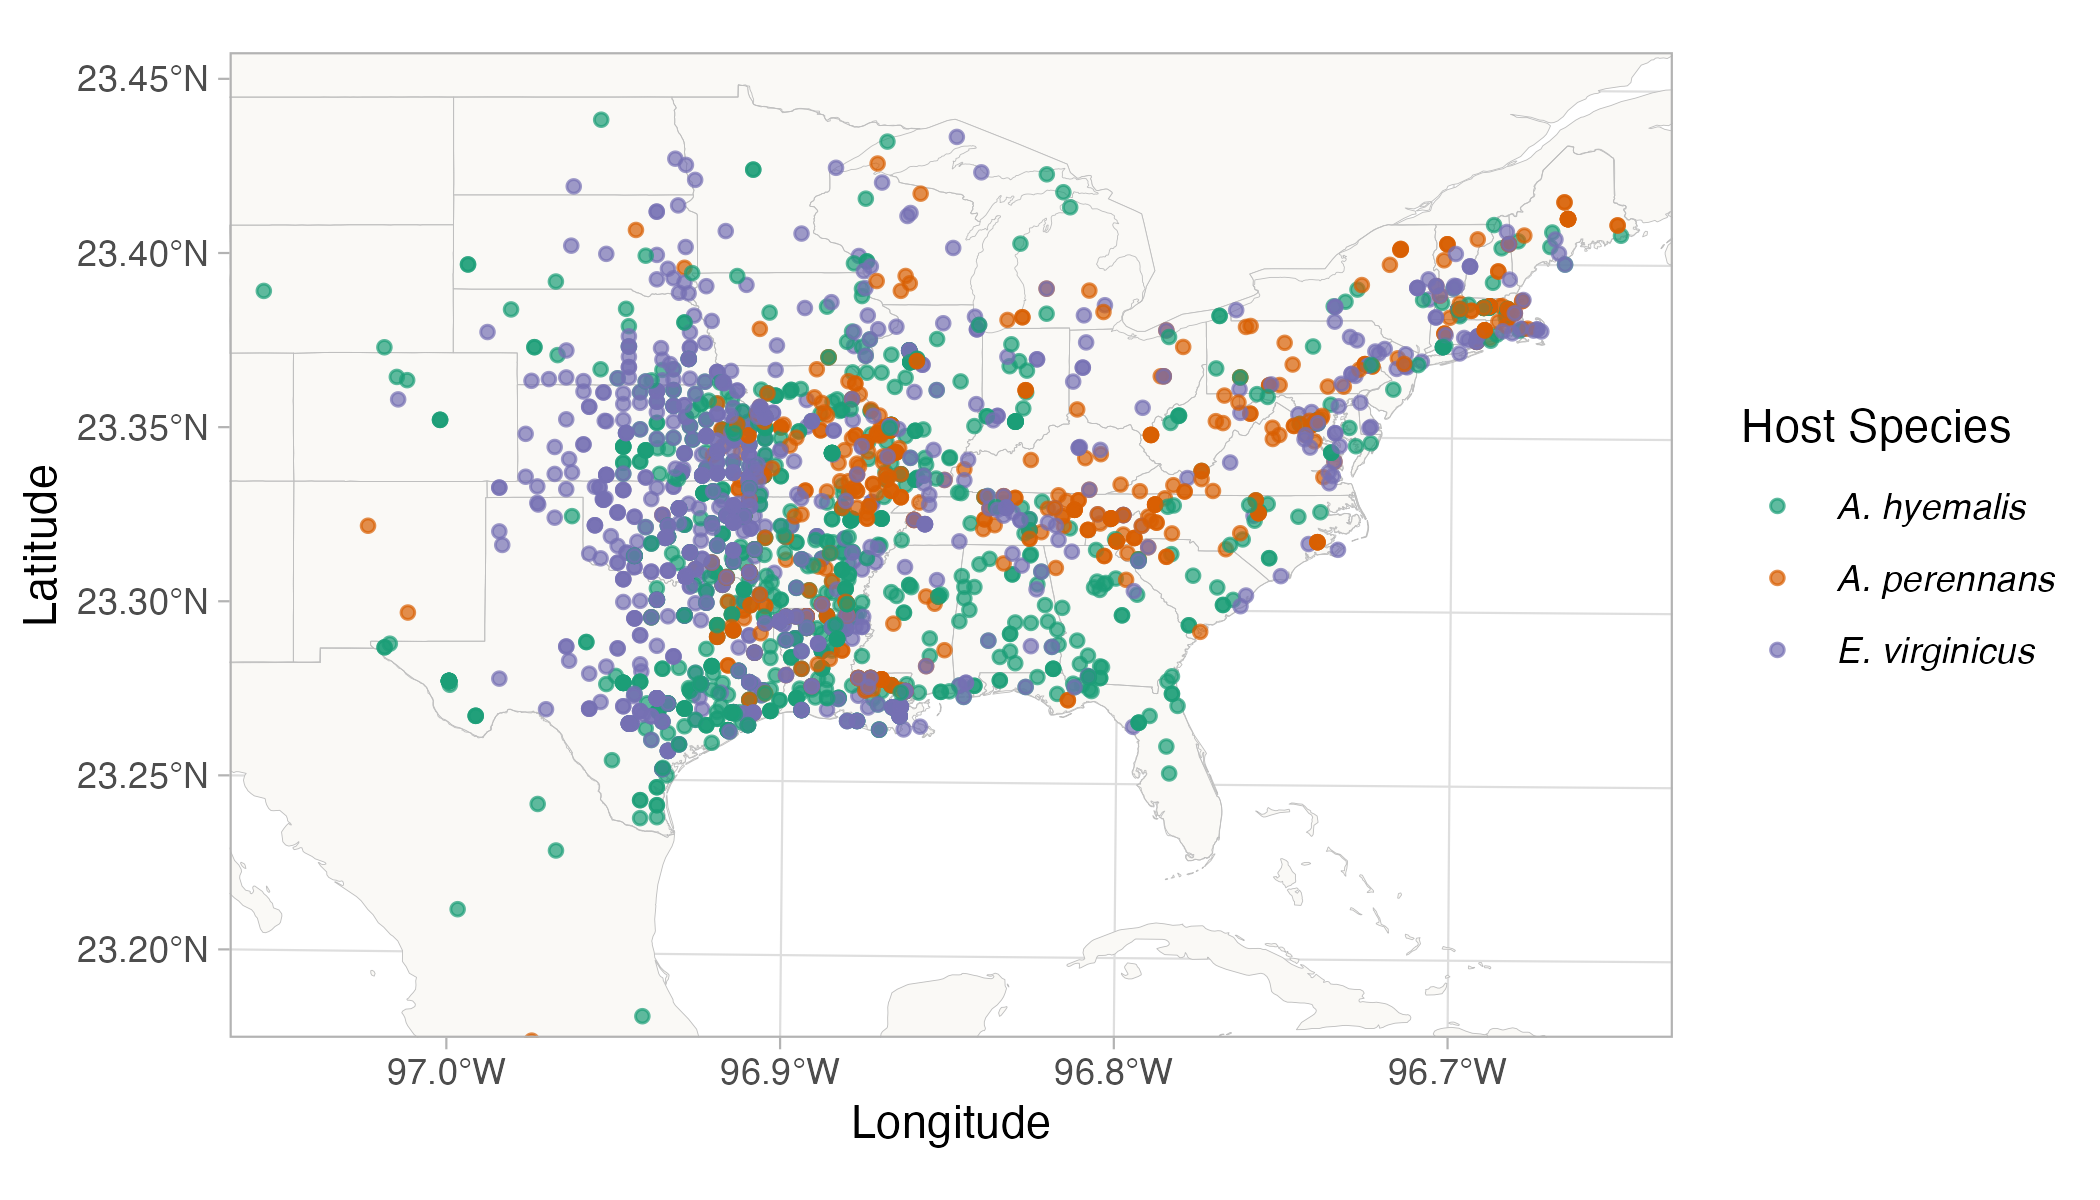
\includegraphics[width = \linewidth]{../Plots/collections_map.png}
	\caption[Collection locations of herbarium specimens sampled for \emph{Epichloë} endophytes]{\textbf{Collection locations of herbarium specimens sampled for \emph{Epichloë} endophytes.} Specimens span eastern North America from nine herbaria, and are colored by host species.}
	\label{fig:map}
\end{figure}


\subsection*{Modeling spatial and temporal changes in endophyte prevalence}
We assessed spatial and temporal changes in endophyte prevalence across each host distribution, quantifying the ``global'' temporal trends aggregated across space, and then examining spatial heterogeneity in the direction and magnitude of endophyte change (hotspots and coldspots) across the spatial extent of each host's distribution.
To account for the spatial non-independence of geo-referenced occurrences, we used an approximate Bayesian method, Integrated Nested Laplace Approximation (INLA), to construct spatio-temporal models of endophyte prevalence.
INLA provides a computationally efficient method of ascertaining parameter posterior distributions for certain models that can be formulated as latent Gaussian Models \cite{rue2009approximate}.
Many common statistical models, including structured and unstructured mixed-effects models, can be represented as latent Gaussian Models.
We incorporated spatial heterogeneity into this analysis using spatially-structured intercept and slope parameters implemented as stochastic partial differential equations (SPDE) to approximate a continuous spatial Gaussian process. 
This SPDE approach is a flexible method of smoothing across space while explicitly accounting for spatial dependence between data-points \citep{lindgren2011explicit,bakka2018spatial}.
Fitting models with structured spatial effects is possible with MCMC sampling but can require long computation times, making INLA an effective alternative. 
This approach has been used to model spatial patterns in flowering phenology \cite{willems2022forest}, the abundance of birds \cite{meehan2019spatial} and butterflies \cite{crossley2022opposing}, the distribution of temperate trees \cite{engel2022spatial} as well as the population dynamics of endangered amphibians \cite{knapp2016large} and other ecological processes \cite{beguin2012hierarchical}.
%\tom{}{Probably not necessary if you need space.}

We estimated global and spatially-varying trends in endophyte prevalence using a joint-likelihood model. 
For each host species $h$, endophyte presence/absence of the $i^{th}$ specimen ($P_{h,i}$) was modeled as a Bernoulli response variable with expected probability of endophyte occurrence $\hat{P}_{h,i}$.
We modeled $\hat{P}_{h,i}$ as a linear function of intercept $\boldsymbol{A}_h$ and slope $\boldsymbol{T}_{h}$ defining the global trend in endophyte prevalence specific to each host species as well as with spatially-varying intercepts $\alpha_{h,l_{i}} $ and slopes $\tau_{h,l_i}$ associated with location ($l_i$, the unique latitude-longitude combination of the $i$th observation).
The joint-model structure allowed us to ``borrow strength'' across species in the estimation of shared variance terms for the spatially-dependent random effect $\delta_{l_i}$, intended to account for residual spatial variation, and $\chi_{c_i}$ and $\omega_{s_i}$ i.i.d.-random effects indexed for each collector identity ($c_i$), and scorer identity ($s_i$) of the $i^{th}$ specimen.

\begin{equation}
	\label{eq:trends}
		logit(\hat{P}_{h,i}) = \boldsymbol{A}_{h} + \boldsymbol{T}_{h}*year_i  + \alpha_{h,l_{i}} + \tau_{h,l_i}*year_i + \delta_{l_i} + \chi_{c_i} + \omega_{s_i} 
\end{equation}

By including random effects for collectors and scorers, we accounted for ``nuisance'' variance that may bias predictions for changes in endophyte prevalence.
Previous work suggests that behavior of historical botanists may introduce biases into ecological inferences made from historic collections \cite{kozlov2020biases}. 
Prolific collectors who contribute thousands of specimens may be more or less likely to collect certain species, or specimens with certain traits \cite{daru2018widespread}. 
Similarly, the process of scoring seeds for hyphae involved several student researchers who, even with standardized training, may vary in their likelihood of positively identifying \emph{Epichloë}. 

We performed model fitting using the inlabru R package \citep{bachl2019inlabru}.
Global intercept and slope parameters $\boldsymbol{A}$, and $\boldsymbol{T}$, were given vague priors.
Scorer and collector random effects, $\chi$ and $\omega$, were given penalized complexity priors, with distributions approximating a Normal distribution with standard deviation of 5. 
Each spatially-structured parameter depended on a covariance matrix according to the proximity of each pair of collection locations \citep{lindgren2011explicit,bakka2018spatial}. 
The covariance matrix was approximated using a Mat\'{e}rn covariance function, with each data point assigned a location according to the nodes of a mesh of non-overlapping triangles encompassing the study area (Fig. \ref{fig:meshplot}).
We assessed model fit with visual posterior predictive checks (\ref{fig:overlayplot}) and measurements of AUC (Figs. \ref{fig:ROCtraining}-\ref{fig:ROCtest}).
Priors for the Mat\'{e}rn covariance function, termed ''range" and "variance", define how proximity effects decay with distance.
Results presented in the main text reflect a prior range of $342$ kilometers (i.e. a $50$\% probability of estimating a range less than $342$ kilometers). 
We tested a range of values (from $68$ kilometers to $1714$ kilometers) and meshes (presented in the Supporting Methods), finding that while the magnitude and uncertainty of effects varied, model results were qualitatively similar, i.e. the same direction of effects across space.


%In all cases, posterior modes were \tom{stable}{Assessed how?} and equal to zero, indicating successful numeric convergence.


\subsection*{Modeling distributions of host species}
Because the herbarium records did not encompass the entirety of these host species'ranges, we additionally modeled the geographic distribution of each host species to generate realistic maps on which we could project the predictions of the INLA model.
We followed the ODMAP (overview, data, model, assessment, prediction) protocol \citep{crossley2022opposing} (see Supporting Methods). 
In short, we used presence-only observations of each host species from Global Biodiversity Information Facility (GBIF) between 1990 to 2020.
%To reduce the potential influence of sampling bias and spatial autocorrelation, \tom{we thinned the occurrences to the spatial scale of our selected climatic predictors}{I do not follow.}. 
%We selected climate variables that aligned with our analysis of climatic influences on trends in endophyte prevalence described above.
%\tom{We calculated the mean and standard deviation of seasonal temperature and precipitation across 1990 to 2020. }{FOr what locations? Is this from the whole raster of NA?}
%\tom{Among this suite of variables, we chose to include, which were uncorrelated (Variance Inflation Factor $>$ 0.7) and allowed us to predict the occurrence probability of each host species in space and time.}{Do not follow and sounds circular.}
We fit maximum entropy (MaxEnt) models using the maxent function in the R package dismo \citep{hijmans2017package} using the same set of seasonal climate predictors considered above calculated for the 1990-2020 climate normals: mean and standard deviation of spring, summer, and autumn temperature, and mean and standard deviation of spring, summer, and autumn cumulative precipitation.
%\josh{MaxEnt is preferred because it has been shown to generate response curves with less unpredictable behavior when applied to new climates \citep{hijmans2006ability}.}{possibly could remove this sentence?}
We generated 10,000 pseudo-absences as background points, and split the occurrence data into 75\% for model training and 25\% for model testing.
The performance of models was evaluated with AUC \citep{jimenez2012insights}. 
We found AUC values of 0.862, 0.838, 0.821 respectively  for \emph{Agrostis hyemalis}, \emph{Agrostis perennans}, and \emph{Elymus virginicus} indicating good model fit to data.
To convert the continuous predicted probabilities into binary presence - absence maps on which we projected INLA predictions, we used the  training sensitivity (true positive rate) and specificity threshold (true negative rate) \citep{liu2005selecting}. 
%These binary maps serve as boundaries in presented maps of change in endophyte prevalence, and outline the set of pixels used in our analysis of climate correlates with trends in endophyte prevalence


\subsection*{Assessing the role of climate drivers}
We assessed how the magnitude of climate change may have driven changes in endophyte prevalence by assessing correlations between changes in climate and changes in endophyte prevalence predicted from our spatial model at evenly spaced pixels across the study area.
We first downloaded monthly temperature and precipitation rasters from the PRISM climate group \citep{daly2013prism} covering the time period between 1895 and 2020 using the 'prism' R package \citep{Rprism2015}. 
Prism provides reconstructions of historic climate variables across the United States by spatially-interpolating weather station data \citep{diLuzio2008constructing}. 
We calculated 30-year climate normals for seasonal mean temperature and cumulative precipitation for the recent (1990 to 2020) and historic (1895 to 1925) periods.
We used three four-month seasons within the year (Spring: January, February, March, April; Summer: May; June, July, August; Autumn: September, October, November, December). 
This division of seasons allowed us to quantify differences in climate associated with the two ``cool'' seasons, when we expected our focal species to be most biologically active (\emph{A. hyemalis} flowering phenology: spring; \emph{E. virginicus}: spring and summer; \emph{A. perennans}: autumn). 
In addition to mean climate conditions, environmental variability itself can influence population dynamics \cite{tuljapurkar_population_1982} and changes in variability are a key prediction of climate change models \cite{stocker2013technical, ipcc_2021}. 
Therefore, we calculated the standard deviation for each annual and seasonal climate driver across each 30-year period.
We then took the difference between recent and historic periods for the mean and standard deviation for each climate driver (Figs. \ref{fig:AGHY_climate_covariates}-\ref{fig:ELVI_climate_covariates}).
All together, we assessed twelve potential climate drivers: the mean and standard deviation of spring, summer, and autumn temperature, as well as the mean and standard deviation of spring, summer, and autumn cumulative precipitation.

To evaluate whether areas that have experienced the greatest changes in endophyte prevalence (hotspots of endophyte change) are associated with high degrees of change in climate (hotspots of climate change), we modeled the fitted, spatially-varying slopes of endophyte change through time ($\tau_{[h]l}$ as a linear function of environmental covariates, with a Gaussian error distribution.
Data from each host species was analyzed separately. 
Fitting regressions to many pixels across the study region risks articially inflating confidence in our results due to large sample sizes, and so we performed this analysis using only a random subsample of 250 pixels across the study region; other sizes of subsample yielded similar results.

\subsection*{Validating model performance with in-sample and out-of-sample tests}
We evaluated the predictive ability of the model using both in-sample training data from the herbarium surveys, and with out-of-sample test data, an important but rarely used strategy in ecological studies \cite{tredennick2021practical, lee2024phenological}.
We generated out-of-sample test data from contemporary surveys of endophyte prevalence in natural populations of \emph{A. hyemalis} and \emph{E. virginicus} in Texas and the southern US. 
Surveys of \emph{E. virginicus} were conducted in 2013 as described in \citet{sneck2017variation}, and surveys of \emph{A. hyemalis} took place between 2015 and 2020.
Population surveys of \emph{A. hyemalis} were initially designed to cover longitudinal variation in endophyte prevalence towards its range edge, while surveys of \emph{E. virginicus} were designed to cover latitudinal variation. 
In total, we visited 43 populations of \emph{A. hyemalis} and 20 populations of \emph{E. virginicus} across the south-central US, with emphasis on Texas and neighboring states (Fig \ref{fig:contempsurveysmap}).
During surveys, we collected seeds from up to 30 individuals per population (average number of plants sampled per population: $22.9$); note that this sampling design provided greater local depth of information than the herbarium records, where only one plant was sampled at each locality.
We quantified the endophyte status of each individual with staining microscopy as described for the herbarium surveys (with 5-10 seeds scored per individual), and calculated the prevalence of endophytes within the population (proportion of plants that were endophyte-symbiotic).
For each population, we compared the observed fraction of endophyte-symbiotic hosts to the predicted probability of endophyte occurrence $\hat{P}$ derived from the model for that location and year. 
The contemporary survey period (2013-2020) is at the most recent edge of the time period encompassed by the historical observations used for model fitting.
%We compared the model's prediction for these locations to the observed population prevalence.

		
\section*{Results}
\subsection*{How has endophyte prevalence changed over time?}
Across >2300 herbarium specimens dating back to 1824, we found that prevalence of \emph{Epichloë} endophytes increased over the last two centuries for all three grass host species (Fig. \ref{fig:temporal}). 
On average, endophytes of \emph{A. perennans} and \emph{E. virginicus} increased from $\sim 40$ \% to  $70$\% prevalence across the study region, and \emph{A. hyemalis} increased from $\sim 25$\% to over $50$\% prevalence.
Our model indicates a high certainty that overall temporal trends are positive across species (99\% probability of a positive overall year slope in \emph{A. hyemalis}, 92\% probability of a positive overall year slope in \emph{A. perennans}, and 91\% probability of a positive overall year slope in \emph{E. virginicus}) (Fig. \ref{fig:temporal_posterior}). 

\begin{figure}[H]
	\centering
	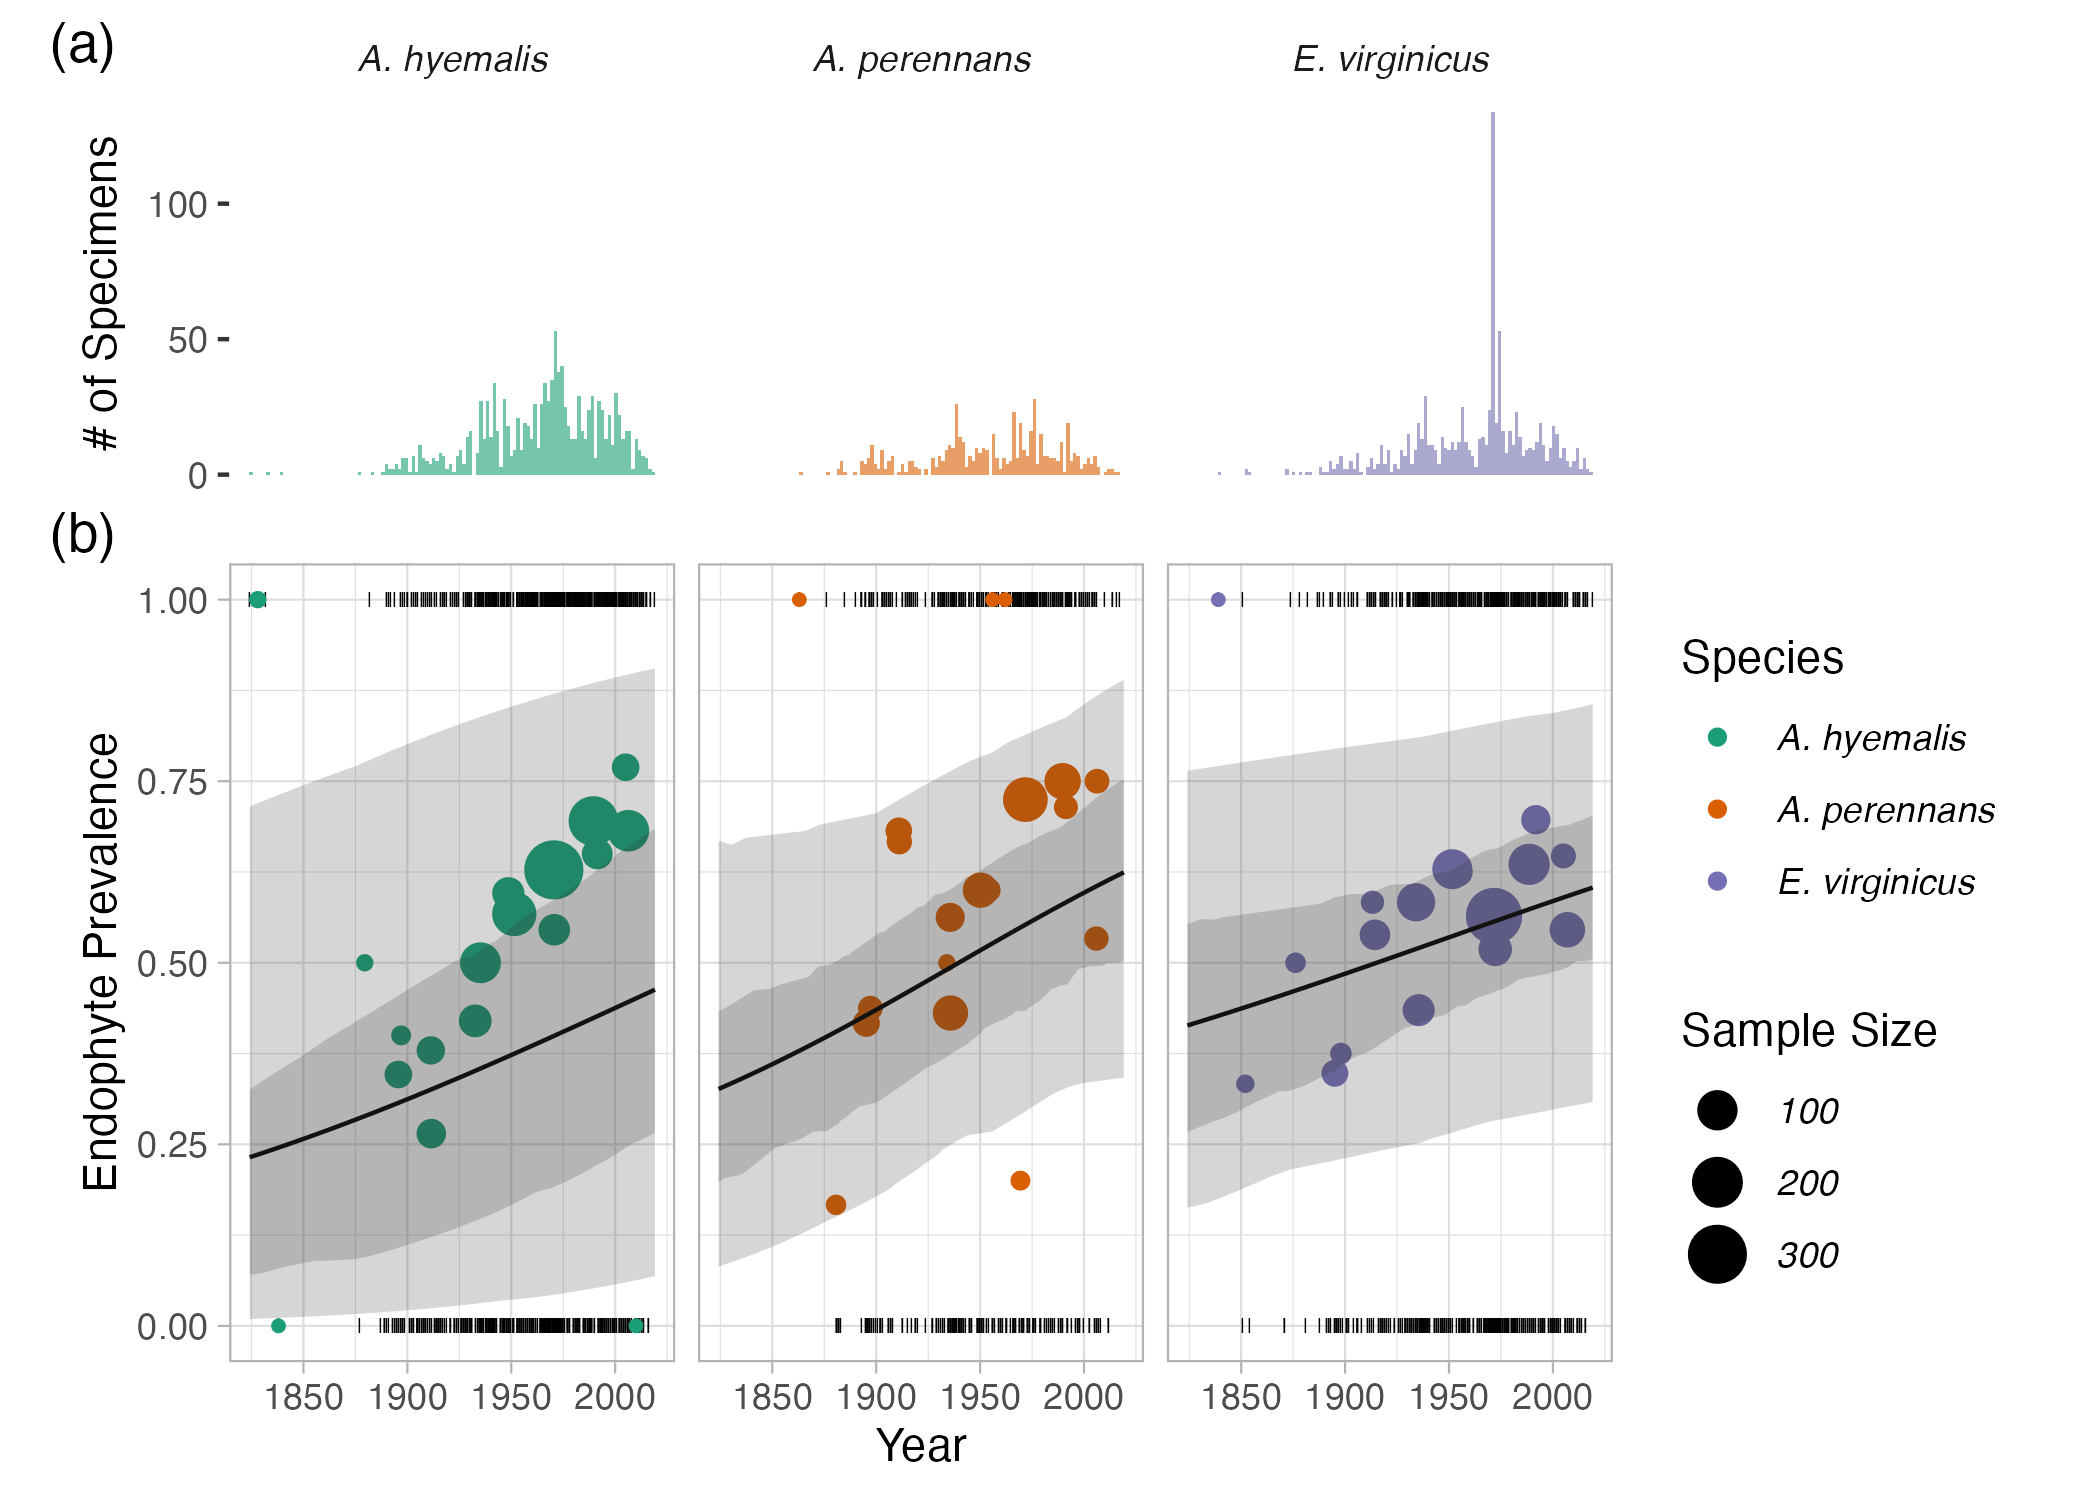
\includegraphics[width = \linewidth]{../Plots/year_plot.png}
	\caption[Temporal trends in endophyte prevalence.]{\textbf{Temporal trends in endophyte prevalence.} (A) Histograms show the frequency of scored specimens through time for each host species. (B) Lines show predicted mean endophyte prevalence over the study period along with the 50\%  and 95\% CI bands incorporating uncertainty associated with collector and scorer random effects. Colored points are binned means of the observed endophyte presence/absence data (black dashes). Colors represent each host species and point size represents the number of specimens.}
	\label{fig:temporal}
\end{figure}


The model appears to under-predict the observed increase in endophyte prevalence relative to the data, particularly for \emph{A. hyemalis} (Fig. \ref{fig:temporal}B), but the model is accounting for random effects and spatial non-independence that are not readily seen in the figure. 
We found no evidence that collector biases influenced our results. 
Collector random effects were consistently small (Fig. \ref{fig:collector_fx}), and models fit with and without this random effect provide qualitatively similar results.
The identity of individual scorers did contribute to observed patterns in endophyte prevalence.
For example, $3$ of the $25$ scorers were more consistently likely than average to assign positive endophyte status, as indicated by 95\% credible intervals greater than zero (Fig. \ref{fig:scorer_fx}). 
It is difficult to distinguish whether this was driven by true differences in scorers biases during the seed scoring process or by unintended spatial or temporal clustering of the specimens scored by each scorer \cite{clayton1993spatial,urdangarin2023evaluating}. 
By under-weighting endophyte-positive samples that are clustered spatially or by collector or observer, the INLA model is appropriately accounting for nuisance variables and providing a conservative inference of endophyte change relative to the raw data. 


\subsection*{How spatially variable are temporal trends in endophyte prevalence?}
While there was an overall increase in endophyte prevalence, our model revealed hotspots and coldspots of change across the host species' ranges, which are mapped in Fig. \ref{fig:svc_time_map} across geographic ranges predicted by MaxEnt species distribution models.
In some regions, posterior mean estimates of spatially varying temporal trends indicate that \emph{A. hyemalis} and \emph{A. perennans} experienced increases in prevalence by as much as $2$\% per year over the study period, while  \emph{E. virginicus} experienced increases up to around $1$\% per year. 
Both \emph{Agrostis} species show areas of strong increase and areas of declining prevalence, while \emph{E. virginicus} had an overall weaker and geographically more homogeneous increase in endophyte prevalence.
Notably, endophytes increased most strongly towards the western range edge of \emph{A. hyemalis} (Fig. \ref{fig:svc_time_map}A) and across the northeastern US for \emph{A. perennans} (Fig. \ref{fig:svc_time_map}B). 
Posterior estimates of uncertainty in spatially varying slopes indicate that these hotspots of change may have experienced increases of up to $5$\% per year while declines in prevalence may be as great as $4$\% per year for \emph{A. hyemalis} and \emph{A. perennans}.
For \emph{E. virginicus}, uncertainty ranges between $3.5$\% increases and $2.5$\% decreases (Fig. \ref{fig:svc_time_map_CI}).

\begin{figure}[H]
	\centering
	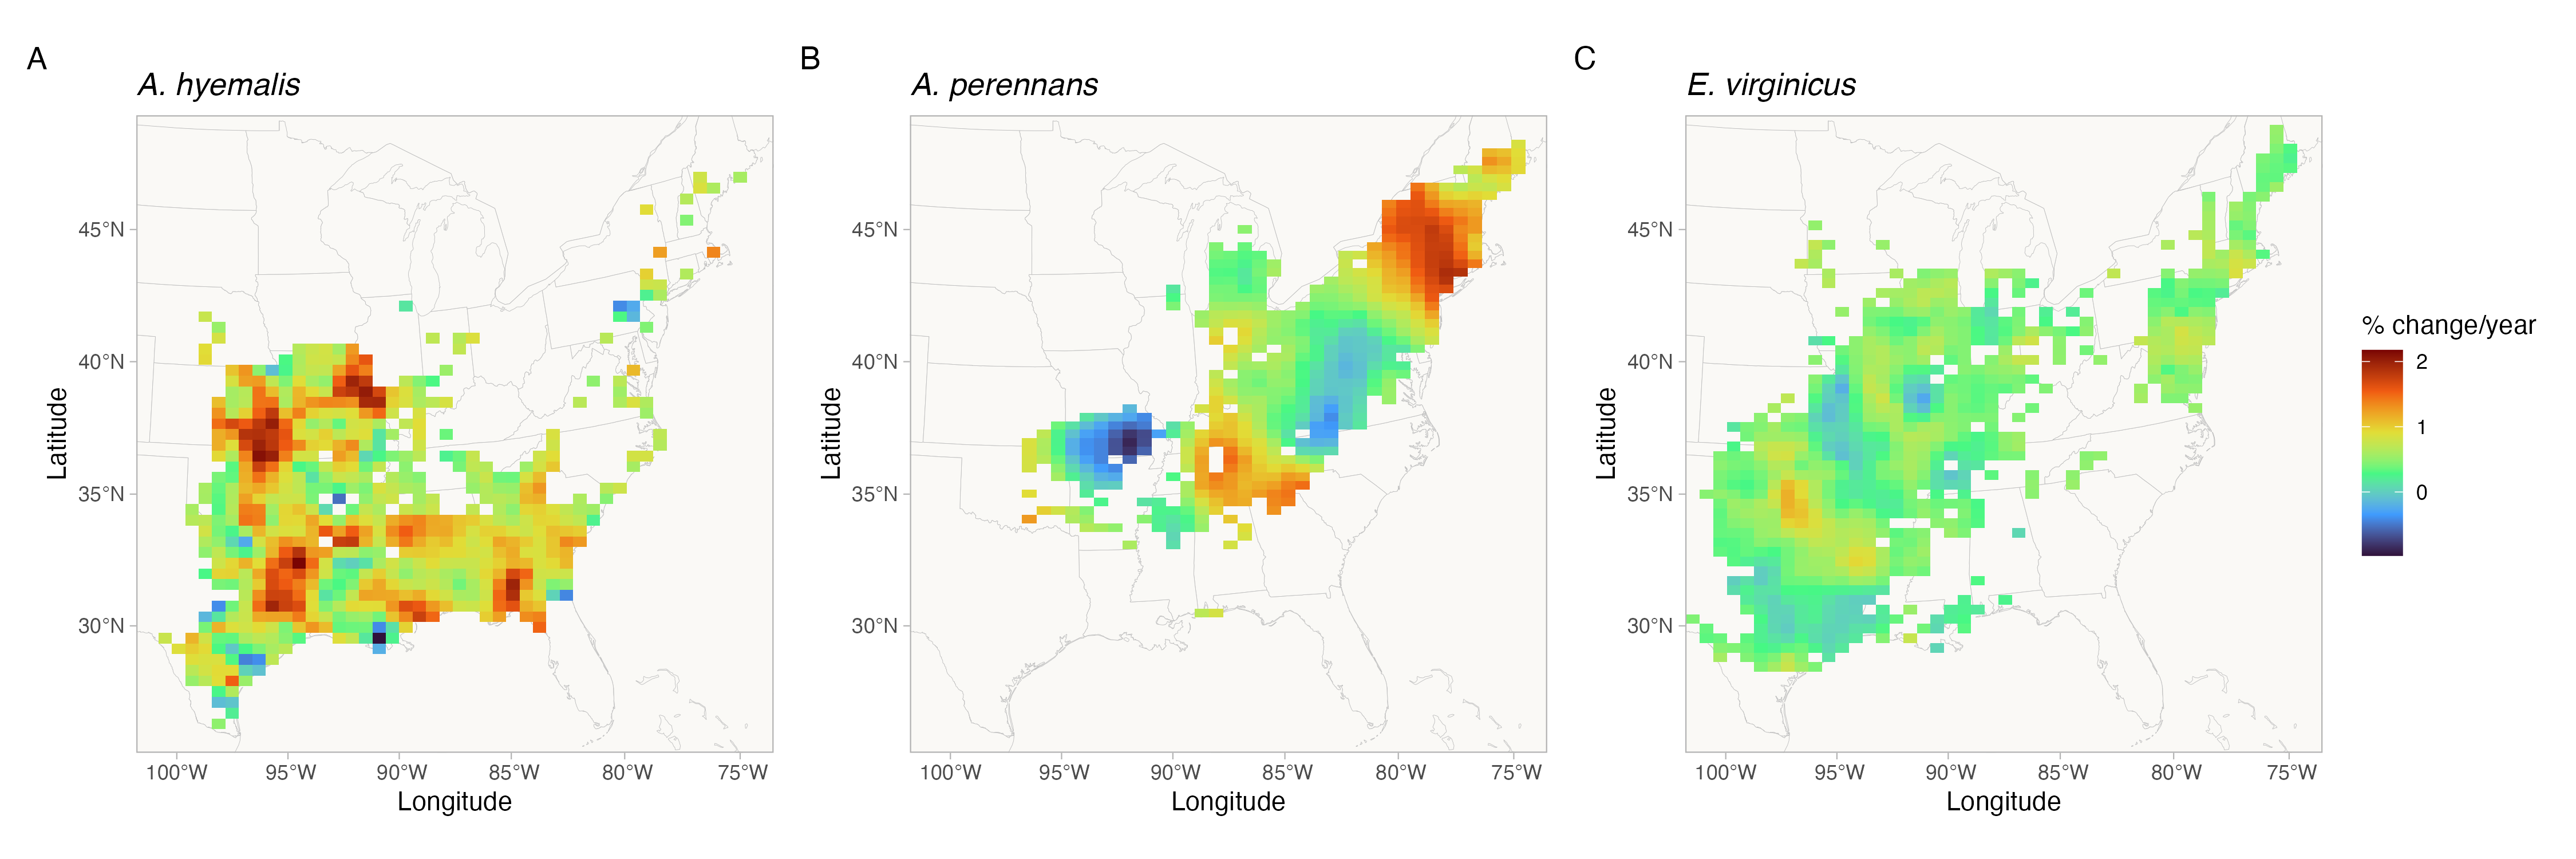
\includegraphics[width = \linewidth]{../Plots/svc_time_map.png}
	\caption[Predicted posterior mean of spatially-varying slopes representing change in endophyte prevalence for each host species.]{Predicted posterior mean of spatially-varying slopes representing change in endophyte prevalence for each host species. Color indicates the relative change in predicted endophyte prevalence.}
	\label{fig:svc_time_map}
\end{figure}



%\subsubsection*{How does endophyte prevalence vary across space?}
%Across space, there were clear trends in endophyte prevalence which varied between species (Fig. 5).
%We mapped predictions of endophyte prevalence across the area encompassing the sampled herbarium specimens for each species, and area smaller than the full geographic distribution of each species in nature.
%\emph{Elymus virginicus} had higher prevalence towards the northern portions of the collection range. 
%In contrast, \emph{Agrostis hyemalis} had highest prevalence towards the center of its collection range with regions of low prevalence towards the northeast and towards its western range edge.
%\emph{Agrostis perennans} had  highest prevalence towards the westernmost portion of its collection range.
%There is considerable uncertainty in the spatial pattern of endophyte prevalence (See Fig. A10 for projections of the 95\% credible interval), however these broad spatial patterns are consistent across the low and high end of model predictions. 

%\begin{figure}[H]
%	\label{fig:svc_space_map}
%	\centering
%	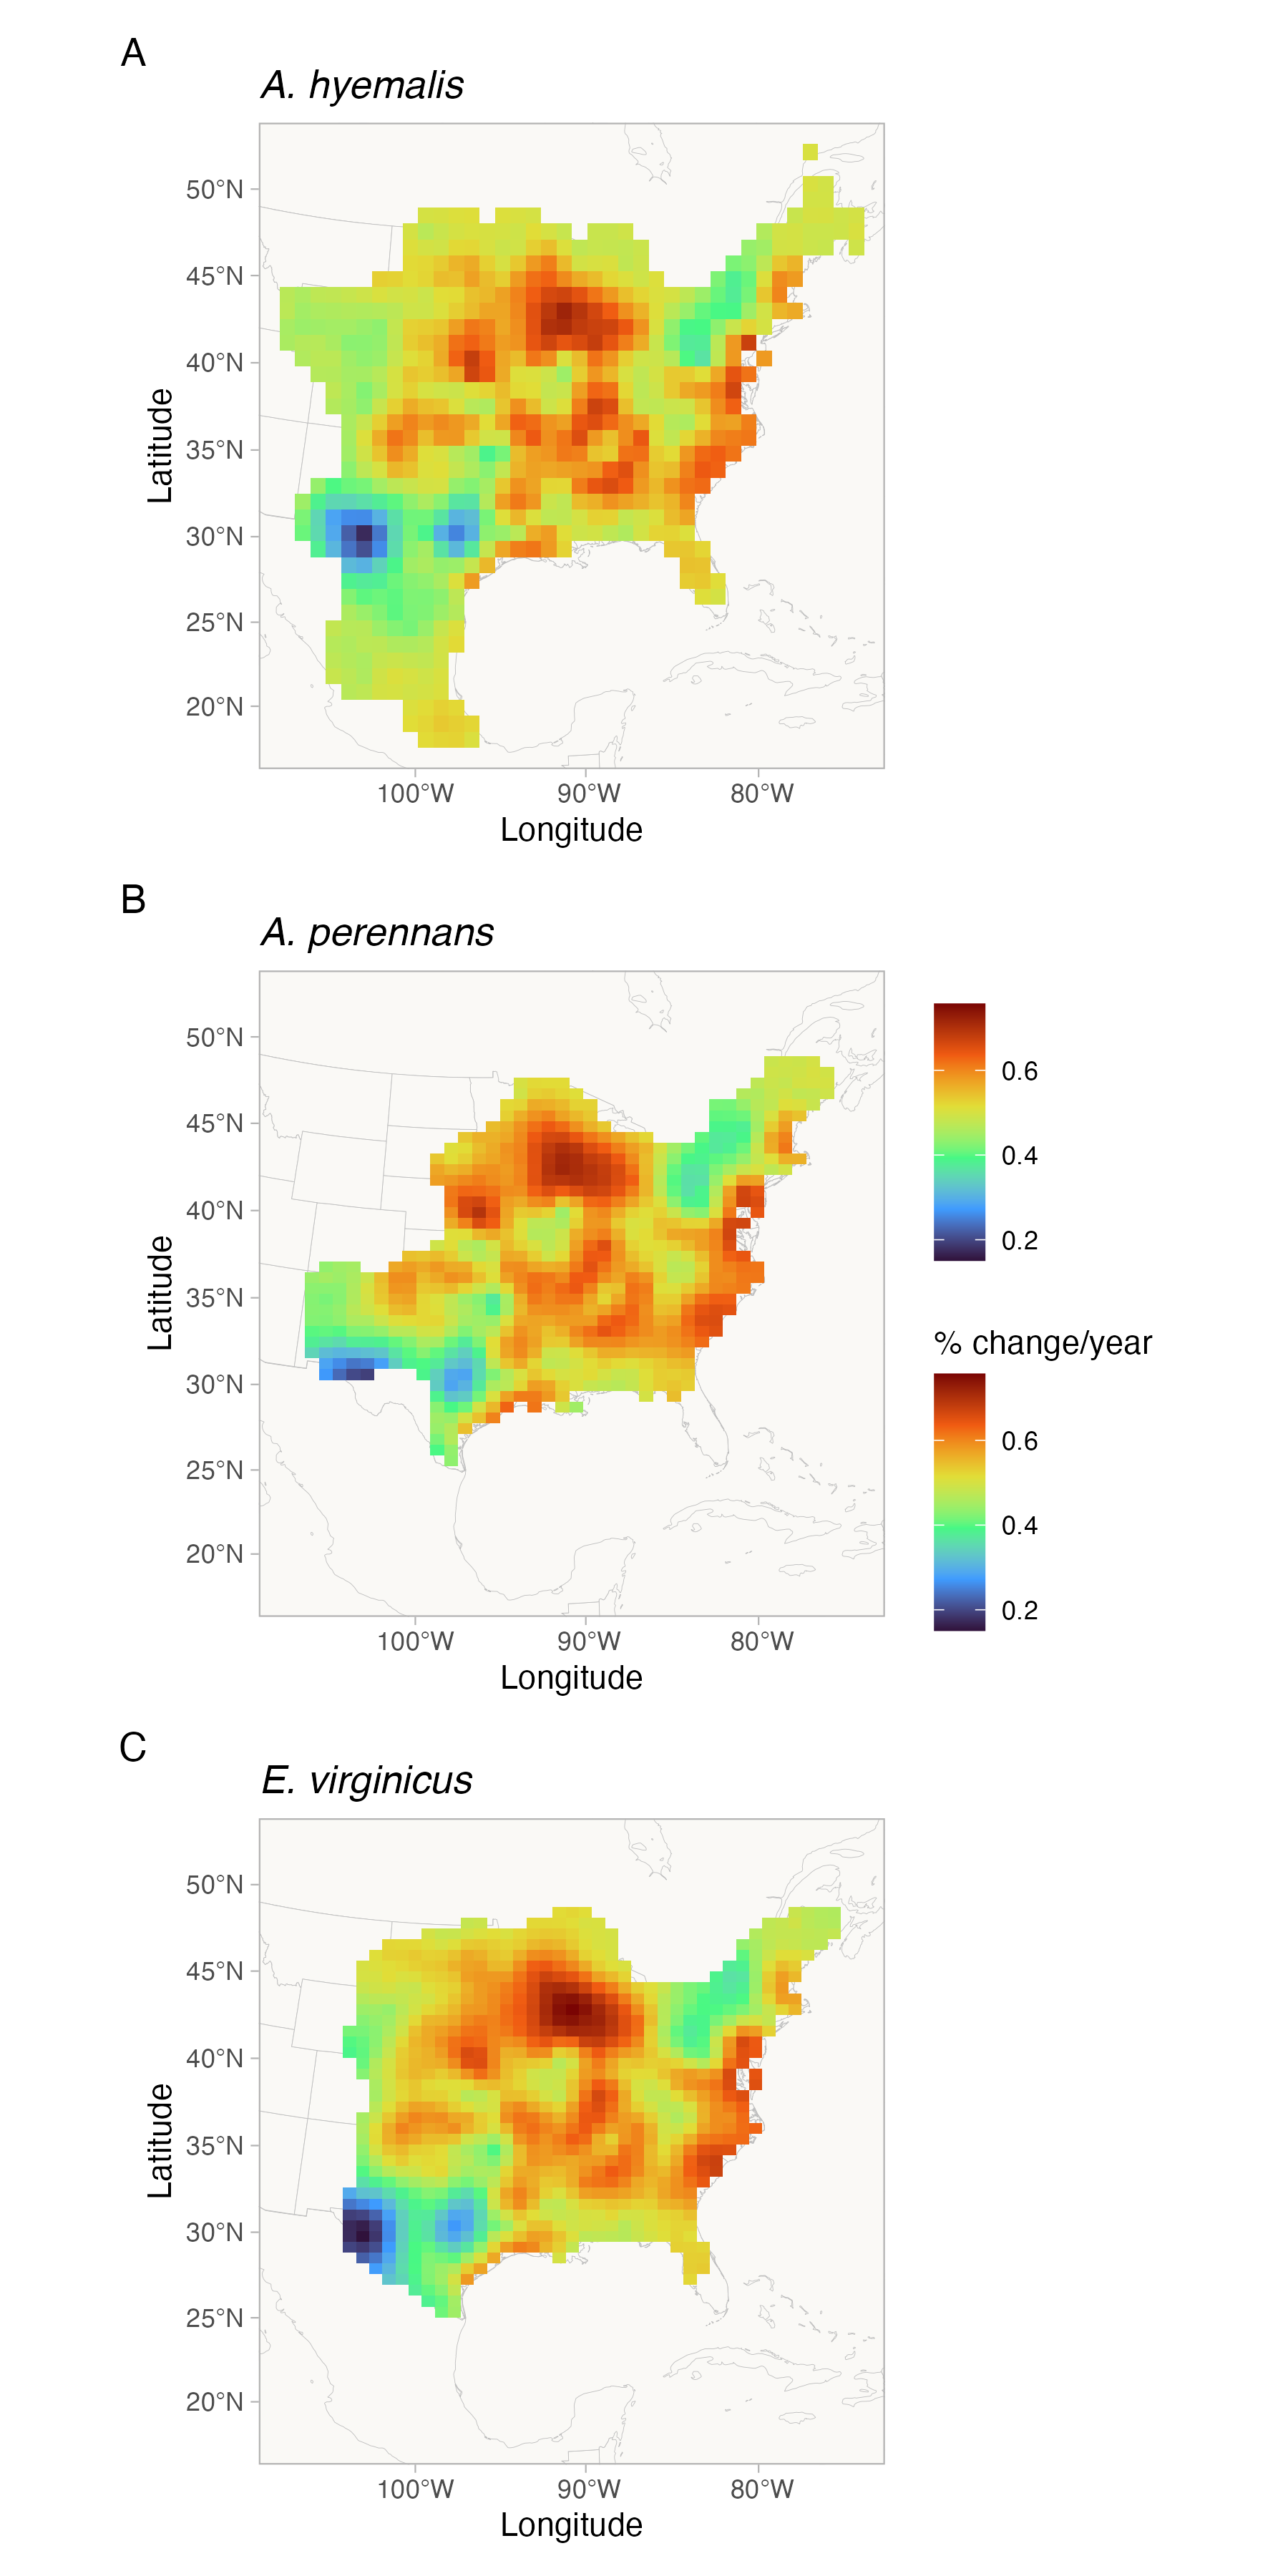
\includegraphics[width = .6\linewidth]{svc_space_map.png}
%	\caption{\textbf{Mean predicted endophyte prevalence for each host species (columns) in 1925 (top row) and 2020 (bottom row)}. Color indicates mean predicted rate of endophyte prevalence across the predicted distribution of each species.}
%\end{figure}





\subsection*{What is the relationship between variation in temporal trends in endophyte prevalence and changes in climate drivers?}
We found that trends in endophyte prevalence were strongly associated with seasonal climate change drivers (Fig. \ref{fig:climate_correlation_plot}).
For the majority of the study region, the climate has become wetter (an average increase in annual precipitation of $60$ mm.) with relatively little temperature warming (an average increase in annual temperature of $0.02$ $^{\circ}$C) over the last century (Fig. \ref{fig:AGHY_climate_covariates}-\ref{fig:ELVI_climate_covariates}), a consequence of regional variation in global climate change \cite{ipcc_2021}. 
Within the region, climate changes were spatially variable; certain locations experienced increases in annual precipitation as large as $375$ mm. or decreases up to $54$ mm. across the last century, while annual temperature changes ranged from warming as great as $1.4$ $^{\circ}$C to cooling by $0.46$ $^{\circ}$C.
Spatially variable climate trends were predictive of trends in endophyte prevalence.
For example, strong increases in endophyte prevalence for \emph{A. perennans} were most strongly associated with increasing autumn precipitation and with increasing mean and variability in autumn temperature (greater than 97\% posterior probabilities of positive slopes).
For this species, a $1$ $^{\circ}$C increase in autumn temperature was associated with a $1.07$ \% increase per year in endophyte prevalence (Fig. \ref{fig:climate_correlation_plot}A) and a $100$ mm. increase in precipitation was associated with a $0.8$\% increase per year in endophyte prevalence (Fig. \ref{fig:climate_correlation_plot}B).
This result aligns with the species' autumn active growing season, however other seasonal climate drivers were also associated with increasing endophyte prevalence. 
In particular, we found cooler and drier springs and cooler summers to be associated with increasing endophyte prevalence (greater than $99$\% posterior probabilities of negative slopes) however these slopes were generally of smaller magnitude than those for autumn climate drivers.

Changes in endophyte prevalence across the ranges of \emph{A. hyemalis} and \emph{E. virginicus} were less strongly driven by changes in climate. 
Like \emph{A. perennans}, climate during peak growing season (spring for \emph{A. perennans} and summer for \emph{E. virginicus}) emerged most commonly as drivers of changes in endophyte prevalence.
Increases in mean spring preciptation were the strongest predictor of increasing trends in endophyte prevalence for \emph{A. hyemalis} (Fig. \ref{fig:climate_correlation_plot}B) (greater than $99$\% posterior probability of a positive slope).
For this species, an increase of $100$ mm. in spring precipitation led to an increase of $0.6$\% per year in endophyte prevalence.
The next greatest slopes were those associated with variability in spring precipitation (greater than $96$\% posterior probability of a negative slope), as well as in the mean and variability of autumn climate (greater than $98$\% probability of negative and positive slopes, respectively). 
Changes in endophyte prevalence in \emph{E. virginicus} were not strongly associated with changes in most climate drivers, but regions with reduced variability in autumn precipitation (Fig. \ref{fig:climate_correlation_plot}B) and with cooler and more variable summer temperatures (Fig. \ref{fig:climate_correlation_plot}A,C) experienced the largest increases in endophyte prevalence.
While our analysis identified the importance of these drivers with relatively high certainty (greater than $99$\% posterior probability of either negative or positive slopes respectively), they translate to less than $0.2$\% change in endophyte prevalence per year for a change of $100$ mm. change in precipitation over the century.
Repeating this analysis using all pixels across each species' distribution were qualitatively similar to these results.


\begin{figure}[H]
	\centering
	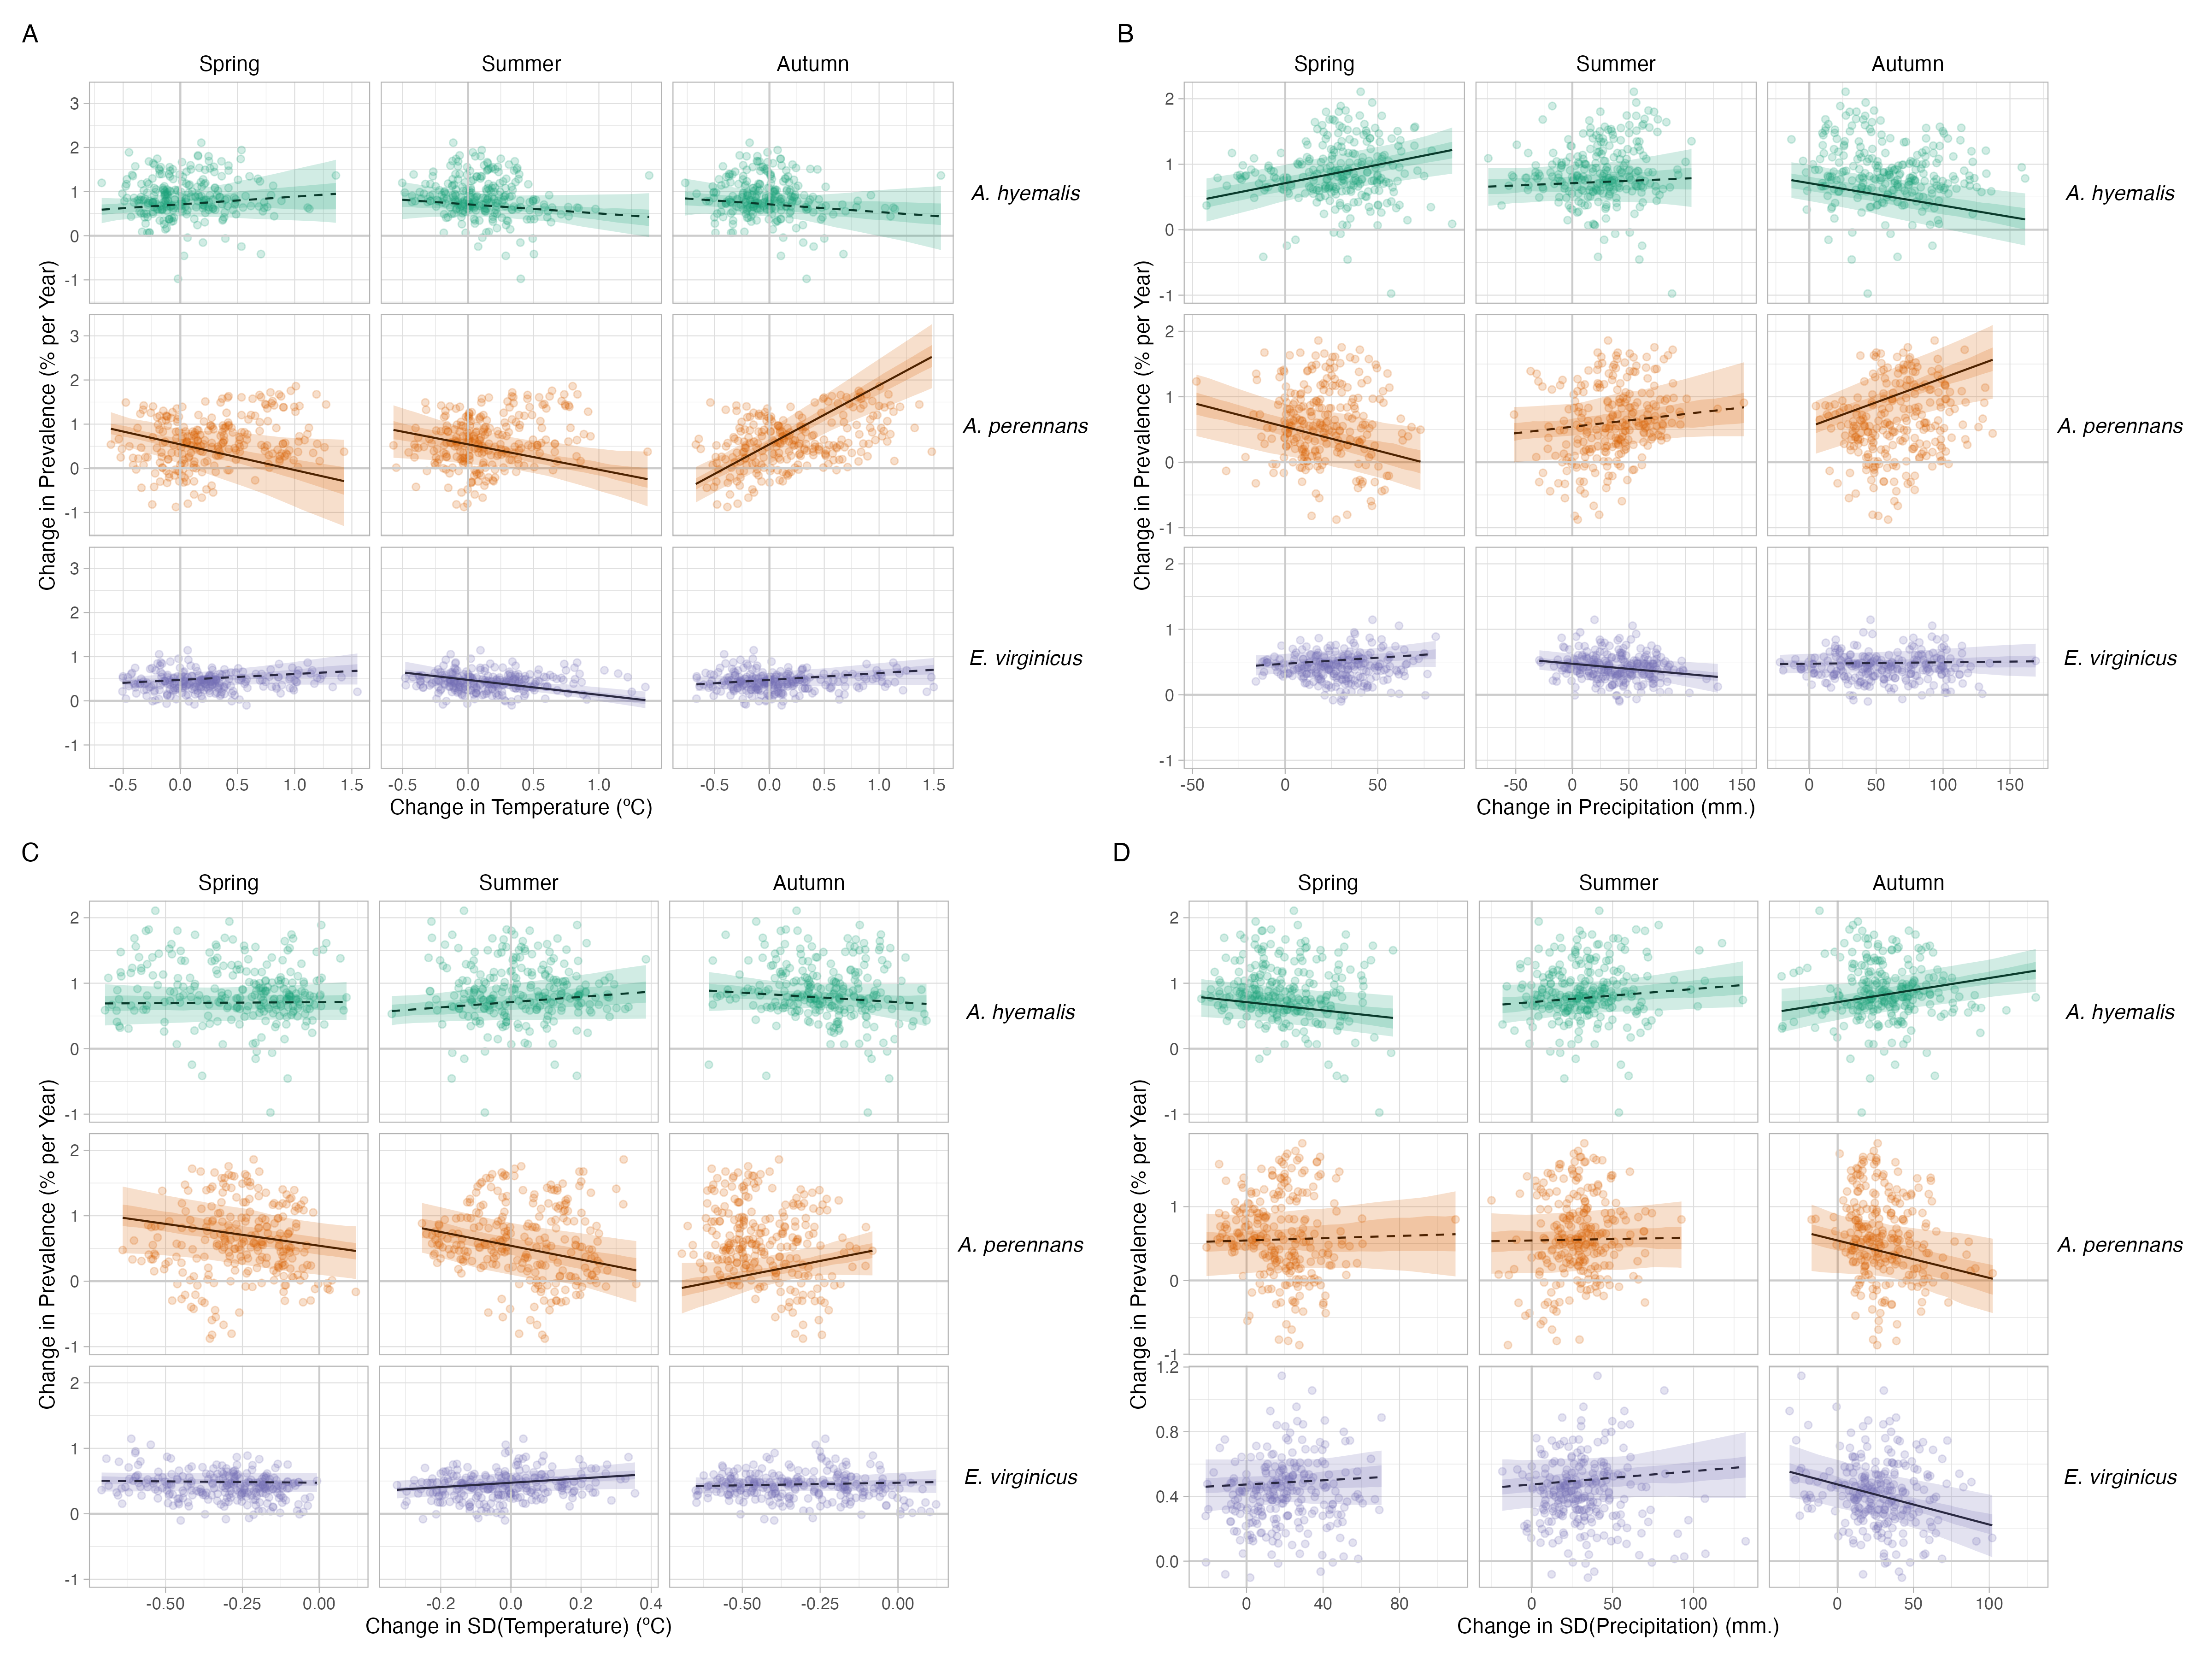
\includegraphics[width = \linewidth]{../Plots/climate_trends_plot_intercept.png}
	\caption[Relationships between predicted trends in endophyte prevalence and changes in seasonal climate drivers.]{\textbf{Relationships between predicted trends in endophyte prevalence and changes in seasonal climate drivers.} Lines show marginal predicted relationship between spatially-varying trends in endophyte prevalence and changes in mean and variability of climate ((A): mean temperature, (B): cumulative precipitation, (C): standard deviation in temperature, (D): standard deviation in precipitation). Confidence bands represent the 50 and 95\% CI,  colored by host species. Slopes with greater than 95\% probability of being either positive or negative are represented as solid lines while those that have less than 95\% probability are dashed. Points show 250 randomly sampled pixels across each host's distribution used in model fitting.}
	\label{fig:climate_correlation_plot}
\end{figure}

\subsubsection*{Performance on test data}
Tests of model's predictive performance as quantified by AUC and by visual posterior predictive checks, indicated good predictive ability. 
Model performance was similar between historic herbarium specimens used as training data and the out-of-sample test data from contemporary surveys (AUC = 0.79 and 0.77 respectively; Fig. \ref{fig:ROCtest}-\ref{fig:ROCtraining}).  
The model successfully captured broad regional trends in endophyte prevalence seen in the contemporary survey data, such as decline endophyte prevalence in \emph{A. hyemalis} towards western longitudes (Fig. \ref{fig:contemptestplot}A) and northern latitudes (Fig. \ref{fig:contemptestplot}B). 
However, model predictions for endophyte prevalence exhibited relatively little local geographic variation, whereas the out-of-sample survey data were maximally variable with populations spanning 0\% to 100\% endophyte-symbiotic plants (Fig. \ref{fig:contemptestplot}C).
We interpret this to mean that the model captures coarse-scale spatial and temporal trends reasonably well, but is not equipped to capture local-scale nuances that generate population-to-population differences. 
%We discuss potential model improvements in the Discussion.

\begin{figure}[H]
	\centering
	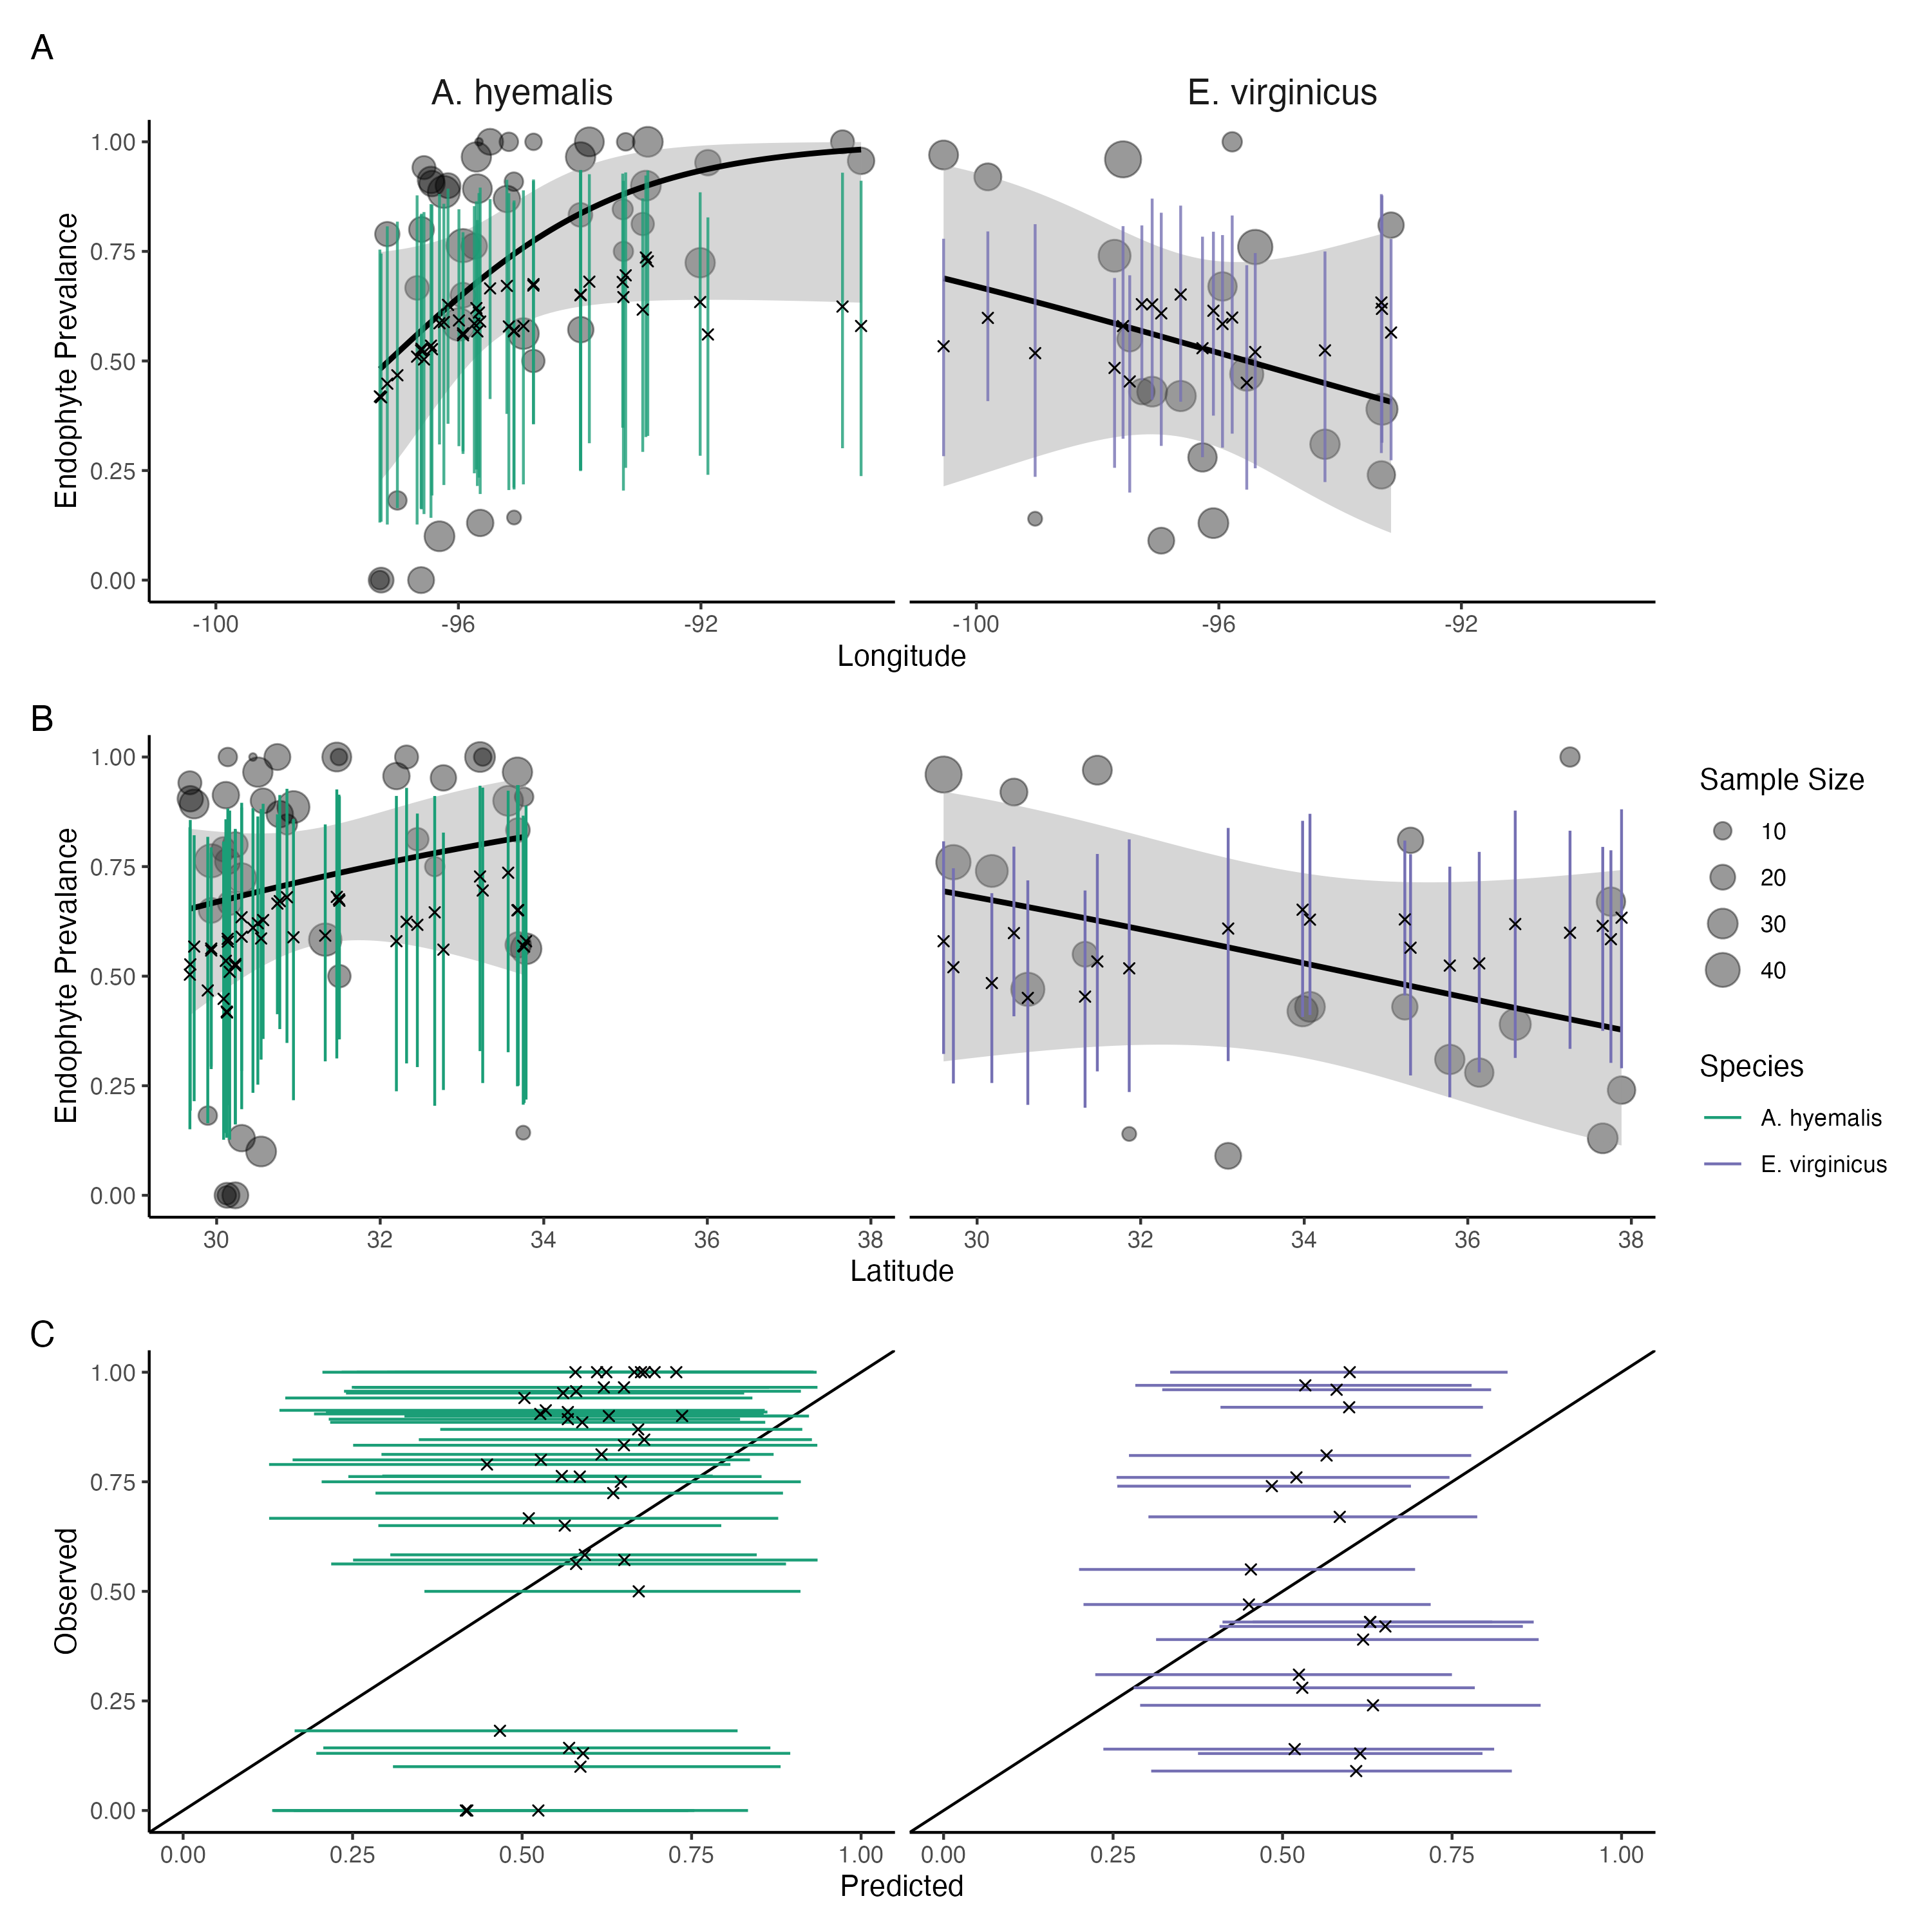
\includegraphics[width = \linewidth]{../Plots/contemp_test_plot.png}
	\caption[Predictive performance for contemporary test data.]{\textbf{Predictive performance for contemporary test data.} (A)
		 The model, trained on historic herbarium collection data, performed modestly at predicting prevalence in contemporary population surveys. The model captured regional trends across (A) longitude and (B) latitude. Crosses indicate predicted mean prevalence along with the 95\% CI (colored lines) from the herbarium model. Contemporary prevalence is represented by grey points (point size reflects sample size) along with trend lines from generalized linear models (black line and shaded 95\% confidence interval). (C) Comparison of observed vs. predicted endophyte prevalence shows that contemporary test data had more variance between populations than contemporary predictions.}
	\label{fig:contemptestplot}
\end{figure}



\section*{Discussion}
Our examination of historic plant specimens revealed cryptic shifts in microbial symbiosis over the last two centuries. 
For the three host species we examined, there have been strong increases in prevalence of fungal endophytes.
We interpret increases in prevalence of \emph{Epichloë}, which are vertically transmitted, as adaptive changes that improve the fitness of their hosts under increasing environmental stress.
This interpretation is in line with theory predicting that the positive fitness feedback caused by vertical transmission leads beneficial symbionts to rise in prevalence within a population \cite{fine1975vectors,donald2021context}.
We further found that trends in endophyte prevalence varied across the distribution of each species in association with changes in climate drivers, suggesting that the increases in endophyte prevalence are driven by context-dependent benefits to hosts that confer resilience under environmental change.
Taken together, this suggests an overall strengthening of host-symbiont mutualism over the last two centuries.

Differences across host species underscore that while all of these $C_3$ grasses share similar broad-scale distributions, each engages in unique biotic interactions and has unique responses to environmental drivers.
We identified hotspots of change for \emph{A. perennans}, which was the species that experienced the strongest absolute changes in endophyte prevalence (Fig. \ref{fig:svc_time_map}).
Declines of $0.9$\% per year in the southern portion of its range and increases of up to $2$\% per year in the north suggest a potential poleward range shift of endophyte-symbiotic plants (whether the overall host distribution is shifting in parallel is an exciting next question). 
Based on previous work demonstrating that endophytes can shield their hosts from drought stress (reviewed in\citet{decunta2021systematic}), we generally predicted that drought conditions would be a driver of increasing endophyte prevalence. 
In contrast to this expectation, increasing prevalence for \emph{A. perennans} were associated with increasing autumn temperature and precipitation (Fig. \ref{fig:climate_correlation_plot}). 
To our knowledge, the response of the symbiosis in \emph{A. perennans} to drought has not been examined experimentally, but in a greenhouse experiment, endophytes had a positive effect on host reproduction under shaded, low-light conditions \citep{davitt2010costs}. 
Our results also hint that it may be useful to investigate whether lagged climate effects are important predictors of host fitness in this system \cite{evers2021lagged}.
Endophyte prevalence of the autumn-flowering \emph{A. perennans} was strongly linked with decreasing spring precipitation, and that of the spring-flowering \emph{A. hyemalis} was associated with decreasing autumn precipitation (Fig. \ref{fig:climate_correlation_plot}B). 
For \emph{A. hyemalis}, endophytes could be playing a role helping hosts weather autumn-season droughts, which may be an important time for the species' germination.
Previous work has demonstrated drought benefits in a greenhouse manipulation with this species \citep{davitt2011understanding}, and early life stages may be particularly vulnerable to prolonged droughts.
%It is possible that the study region has not experienced a magnitude of climate change great enough to cause larger changes in endophyte prevalence for this species. 
%Weak associations with drought could also be explained by climate-driven changes in the rate of imperfect transmission (the generation of non-symbiotic offspring from symbiotic hosts), which could counterbalance endophyte-mediated fitness benefits \citep{donald2021context}. 
For \emph{E. virginicus}, which experienced the most modest changes in endophte prevalence overall (ranging between $1.1$\% increases and $0.2$\% decreases), we only found modest associations with changes in climate drivers. 
Surveys by \citet{sneck2017variation}, used as part of the test data in this study, identified a drought index (SPEI) that integrates precipitation with estimated evapotranspiration as an important predictor of endophyte prevalence.
\emph{Epichloë} endophytes have also been connected to a suite of non-drought related fitness benefits including herbivore protection \citep{brem2001epichloe}, salinity resistence \citep{wang2020effects}, and mediation of the soil microbiome \citep{roberts2015rhizosphere}.
These effects are potentially mediated by the diverse bioactive alkaloids and other signaling compounds they produce \citep{saikkonen2013chemical}.
Increases in symbionts could be explained, at least in part, by these diverse benefits that may help hosts weather a world made increasingly stressful by changes in climate and other anthropogenically introduced stressors.
While we show consistent increasing trends in prevalence between the three species, the mechanisms that explain these changes may be diverse and idiosyncratic.
%This paragraph was a little hard to read and I think does not really nail the points that I think we should make here, IMO. I would open to paragraph setting up the idea that the correlations you detected have some support in previous experimental studies, then elaborate. Then I would acknowledge that other factors can elicit benefits of symbiosis, and these factors may ALSO be changing. The takeaway, for me and perhaps for readers more generally, is that we are very confident endophytes are increasing, we have some confidence that is associated with (and perhaps due to) climate change, but a lot has changed over the past 200 years (climate, urbanization, nitrogen deposition, invasive species, deer!) and we need follow-up studies and experiments to gain a better mechanistic understanding of what has driven these changes, which will also allow us to build better forecasts about the future.


The combination of a spatially-explicit model and historic herbarium specimens allowed us to identify regions of both increasing and decreasing endophyte prevalence, however we see several next steps towards the goal of predicting host and symbiont niche-shifts in response to future climate change.
While the model recreated the large-scale spatial trends observed in contemporary population surveys, test data contained more population-to-population variability in prevalence. 
Validating our model predictions in this way, a rare extra step in collections-based studies, allows us to evaluate places to improve the model's out-of-sample predictive ability.
Lack of information on local variability may simply be a feature of data derived from herbarium specimens. 
They are samples from local populations, but they are single specimens that are aggregated to derive broad-scale model estimates.
This suggests that increasing local replication should be a factor considered in future collection efforts of natural history specimens, balanced with the required time and effort.
Poor predictive ability at local scales in this grass-endophyte system is not surprising, as previous studies have found that local variation, even to the scale of hundreds of meters can structure endophyte-host niches \cite{kazenel2015mutualistic}. 
Other studies have found factors including land-use history \cite{vikuk2019infection} and the biotic environment, including herbivory \cite{rudgers2016long}, and host genotype \citet{sneck2017variation}, to be important predictors of endophyte ecology.
An important step would be integrating data from local and regional scales  through modeling to constrain estimates of local and regional variation.
Previous population surveys have found environment-dependent gradients in endophyte prevalence \citep{sneck2017variation,rudgers2009benefits,semmartin2015broad}, that may be caused by symbiont-derived fitness benefits allowing their hosts to persist in environments where they otherwise could not \citep{afkhami2014mutualist,kazenel2015mutualistic,fowler2023geographic}.
Predicting future niche-shifts of hosts and symbionts will require considering the coupled dynamics of host-symbiont dispersal in addition to fitness benefits.
For example, transplanting symbiotic and non-symbiotic plants beyond the range edge of \emph{A. hyemalis} could tell us whether low endophyte prevalence in that area is a result of environmental conditions that lead the symbiosis to negative fitness consequences, or is a result of some historical contingency or dispersal limitation that has thus far limited the presence of symbiotic hosts from a region where they would otherwise flourish and provide resilience.
Incorporating available climatic and soil layers as covariates is another obvious step that could improve predictions.
These steps will bridge gaps that often exist between large but broad bioclimatic and biodiversity data and small but local data on biotic interactions, and move towards the goal of predicting the dynamics of microbial symbioses under climate change \cite{miller2019recent, isaac2020data}.


Our analysis advances the use of herbarium specimens in global change biology in two ways. 
First and foremost, this is the first study to link long-term changes in microbial symbioses to changes in climate using specimens from natural history collections.
The responses of microbial symbioses are a rich target for future studies within museum specimens, particularly those that take advantage of advances in sequencing technology.
While we used relatively coarse presence/absence data based on fungal morphology, other studies have examined historic plant microbiomes using molecular sequencing and sophisticated bioinformatics techniques, but these studies have so far been limited to relatively few specimens at limited spatial extents \cite{yoshida2015computational,heberling2019utilizing, bieker2020metagenomic,gross2021hidden,bradshaw2021global}. 
Continued advances in capturing historic DNA and in filtering out potential contamination during specimen storage \citep{daru2019novel,bakker2020herbarium,raxworthy2021mining} will be imperative in the effort to scale up these efforts. 
This scaling up will be essential to be able to quantify changes not just in the prevalence of symbionts, but also in symbionts' intraspecific variation and evolutionary responses to climate change, as well as  in changes in the wider microbial community. 
Genetic variation in \emph{Epichloë} endophytes, particularly in genes responsible for alkaloid production, produces ``chemotypes" with differing benefits for hosts against insect or mammalian herbivores mediated by environmental conditions \cite{schardl2012chemotypic,saikkonen2013chemical}.  
With improved molecular insights from historic specimens, we could ask whether the broad increases in endophytes that we have identified reflect selection for particular chemotypes and how this selection varies across space.
Answering these questions as well as the unknown questions that future researchers may ask also reiterates the value in capturing meta-information during ongoing digitization efforts at herbaria around the world and during the accession of newly collected specimens \citep{lendemer2020extended,edwards2024university}.
Second, we accounted for several potential biases in the data observation process that may be common to many collections-based research questions by using a spatially-explicit random effects model. 
Spatial autocorrelation \cite{willems2022forest}, potential biases introduced by the sampling habits of collectors \citep{daru2018widespread}, and variation between contemporary researchers during the collection of trait data, if not corrected for could lead to over-confident inference about the strength and direction of historic change (Fig. \ref{fig:temporal}).
Previous studies that have quantified the effects of collector biases typically find them to be small  \cite{davis2015herbarium,meineke2019herbarium}, and we similarly did not find that collector has a strong effect on the results of our analysis, but that scorer identity did impact results.
%Fitting this model in a Bayesian framework allows for full propagation of uncertainty.

Ultimately, a central goal of global change biology is to generate predictive insights into the future of natural systems on a rapidly changing planet. 
Beyond host-microbe symbioses, detecting ecological responses to anthropogenic global change and attributing their causes would inform public policy decision-makers and adaptive management strategies.
This survey of historic endophyte prevalence is necessarily correlative, yet it serves as a foundation to develop better predictive models of the response of microbial symbioses to climate change. 
By comparing detected ecological responses with alternative mechanistic simulations of the past, we could attribute their cause, in a manner similar to methods from climate science and economics \citep{stott2010detection, carleton2016social,trenberth2015attribution}.
Combining the insights from this type of regional-scale survey with field experiments and physiological performance data could be invaluable to identify mechanisms driving shifts in host-symbiont dynamics.
Evidence is strong that certain dimensions of climate change correlated with endophytes' temporal responses, however we do not know why trends in prevalence were weak in some areas or how endophytes would respond to more extreme changes in climate.
The ``time machine'' of natural history collections revealed evidence of mutualism resilience for grass-endophyte symbioses in the face of environmental change, but more extreme changes could potentially push one or both partners beyond their physiological limits, leading to the collapse of the mutualism; more research is needed to understand what those limits might be. 


	%%%%%%%%%%%%%%%%%%%%%
	% Acknowledgments
	%%%%%%%%%%%%%%%%%%%%%
	% You may wish to remove the Acknowledgments section while your paper 
	% is under review (unless you wish to waive your anonymity under
	% double-blind review) if the Acknowledgments reveal your identity.
	% If you remove this section, you will need to add it back in to your
	% final files after acceptance.
	
	\section*{Acknowledgments}
	We thank Dr. Jessica Budke for help in drafting our initial destructive sampling plan, and to the many staff members of herbaria who facilitated our research visits, as well as to the hundreds of collectors who contributed to the natural history collections. 
	Several high schooler and undergraduate researchers contributed to data collection, including A. Appio-Riley, P. Bilderback, E. Chong, K. Dickens, L. Dufresne, B. Gutierrez, A. Johnson, S. Linder, E. Scales, B. Scherick, K. Schrader, E. Segal , G. Singla, and M. Tucker.
	This research was supported by funding from National Science Foundation (grants 1754468 and 2208857) and by funding from the Texas Ecolab Program.


	%%%%%%%%%%%%%%%%%%%%%
	% Statement of Authorship
	%%%%%%%%%%%%%%%%%%%%%
	% This section should also be commented out while your MS is undergoing
	% double-blind review. The specifics should of course be adapted to
	% your paper, but the paragraph below gives some hints of possible
	% contributions.
	
	\section*{Statement of Authorship}
J.C.F. contributed to research conception, data collection, data analysis, and led manuscript drafting.
J.M. contributed to data analysis and manuscript revisions.
T.E.X.M. contributed to research conception, data collection, data analysis, and manuscript revisions.

	
	\section*{Data and Code Availability}
	Data from this publication can be found through a publicly available repository \josh{()}{will update with the URL}.
	Code for analyses can be found through a publicly available repository (https://github.com/joshuacfowler/EndoHerbarium) that will be permanently archived upon publication.
	
	\section*{Appendix A}
	\renewcommand{\thefigure}{A\arabic{figure}}
	\setcounter{figure}{0}
	
		\renewcommand{\thetable}{A\arabic{table}}
	\setcounter{equation}{0}  % reset counter 
	\setcounter{figure}{0}
	\setcounter{table}{0}
	
	\begin{figure}[H]
		\centering
		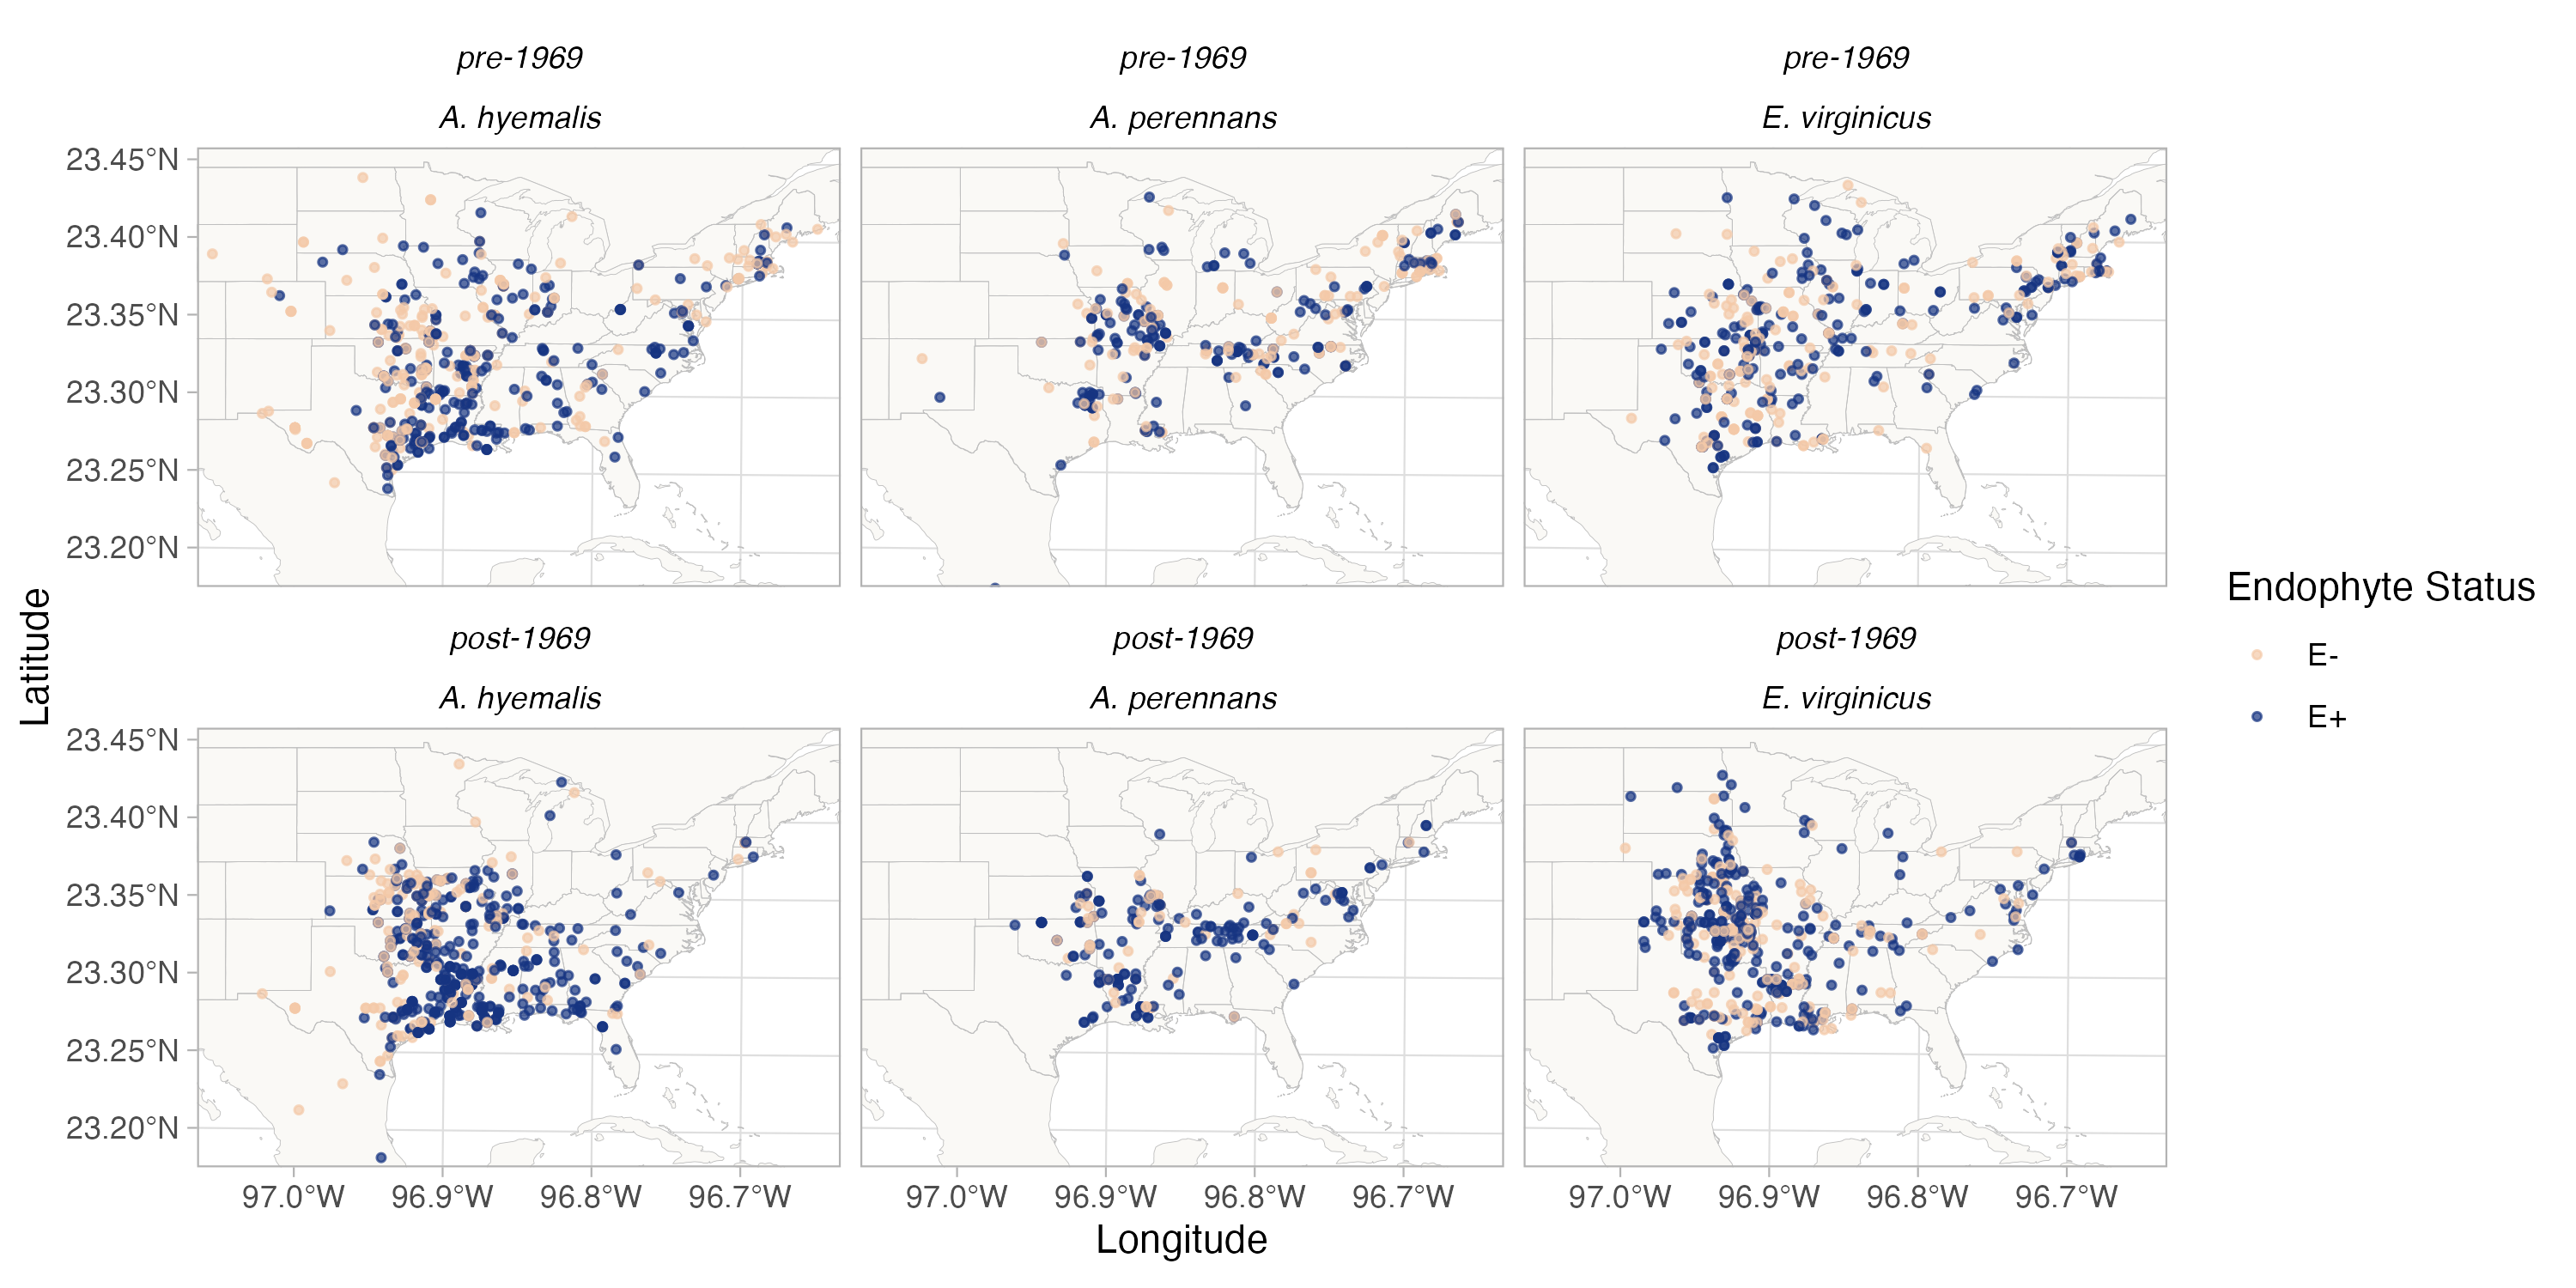
\includegraphics[width = \linewidth]{../Plots/endo_status_map.png}
		\caption{\textbf{Endophyte presence/absence in specimens of each host species.} Points show collection locations colored according to whether the specimen contained endophytes ( E+; blue points) or did not contain endophytes (E-, tan points). To visualize temporal change, the data are faceted before and after the median year of collection.}
		\label{fig:endo_status_map}
	\end{figure}
	
	\begin{figure}[H]
		\centering
		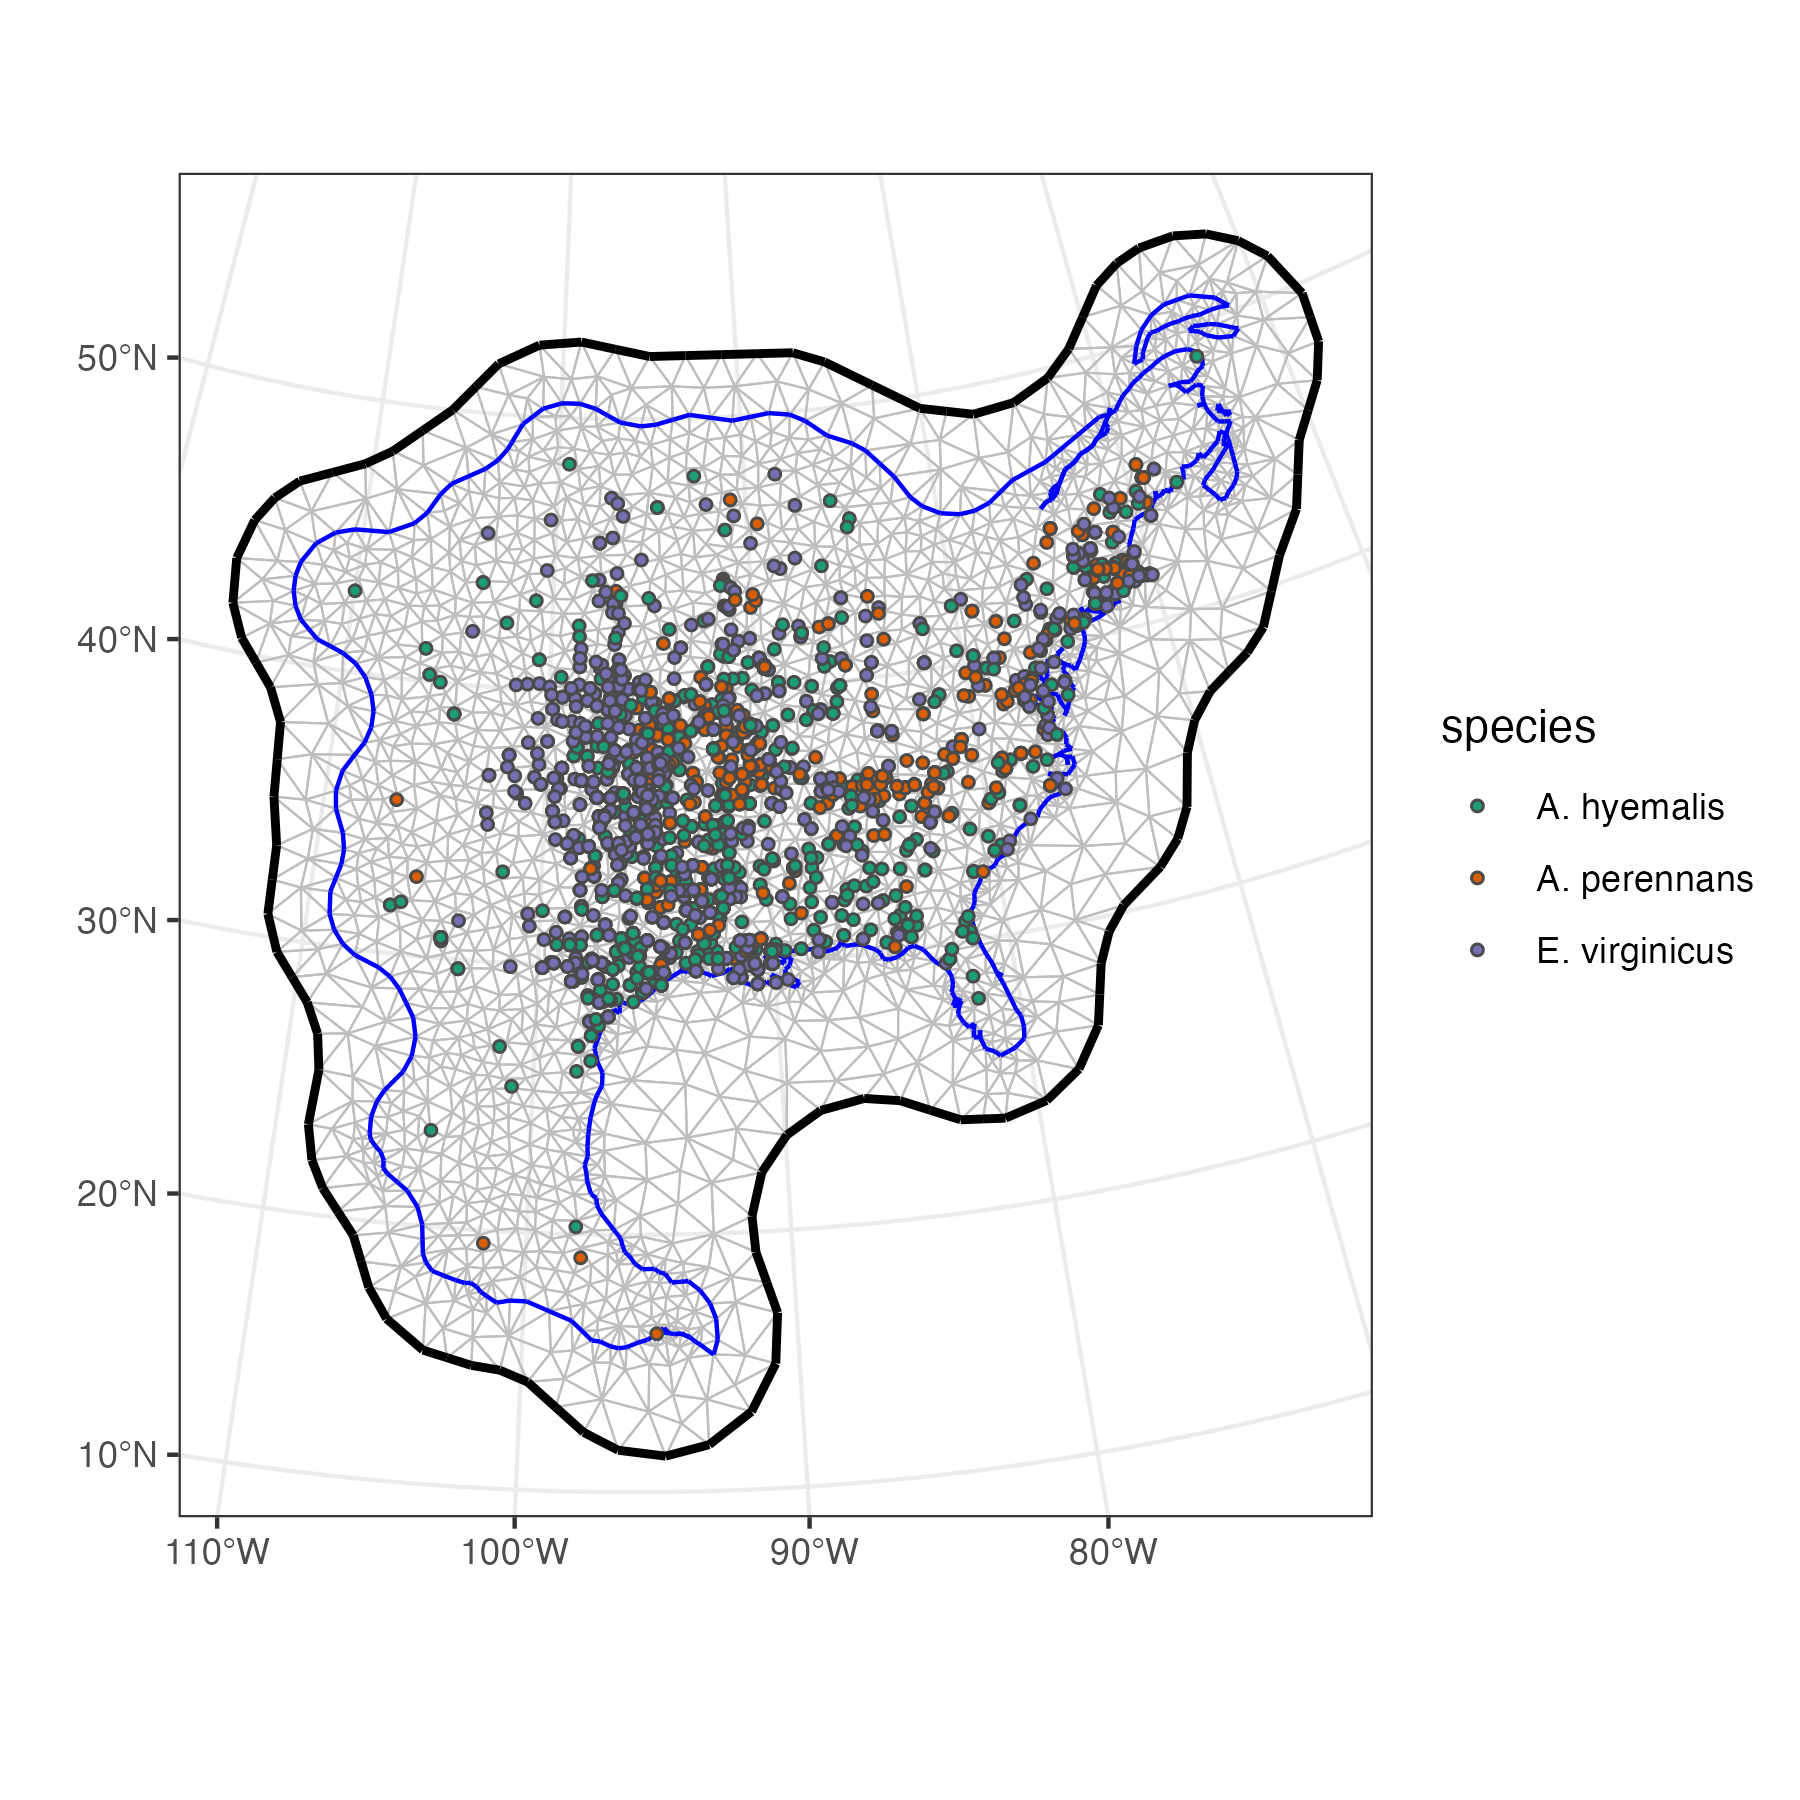
\includegraphics[width = \linewidth]{../Plots/mesh_plot.png}
		\caption{\textbf{Triangulation mesh used to estimate spatial dependence between data points}. Grey lines indicate edges of triangles used to define distances between observations. Colored points indicate locations of sampled herbarium specimens for each host species, and the blue line shows the convex hull and coastline used to define the edge of the mesh around the data points. The thick black line shows the convex hull defining a buffer space around the edge of the mesh to reduce the influence of edge effects on model estimates.}
		\label{fig:meshplot}
	\end{figure}

\begin{figure}[H]
	\centering
	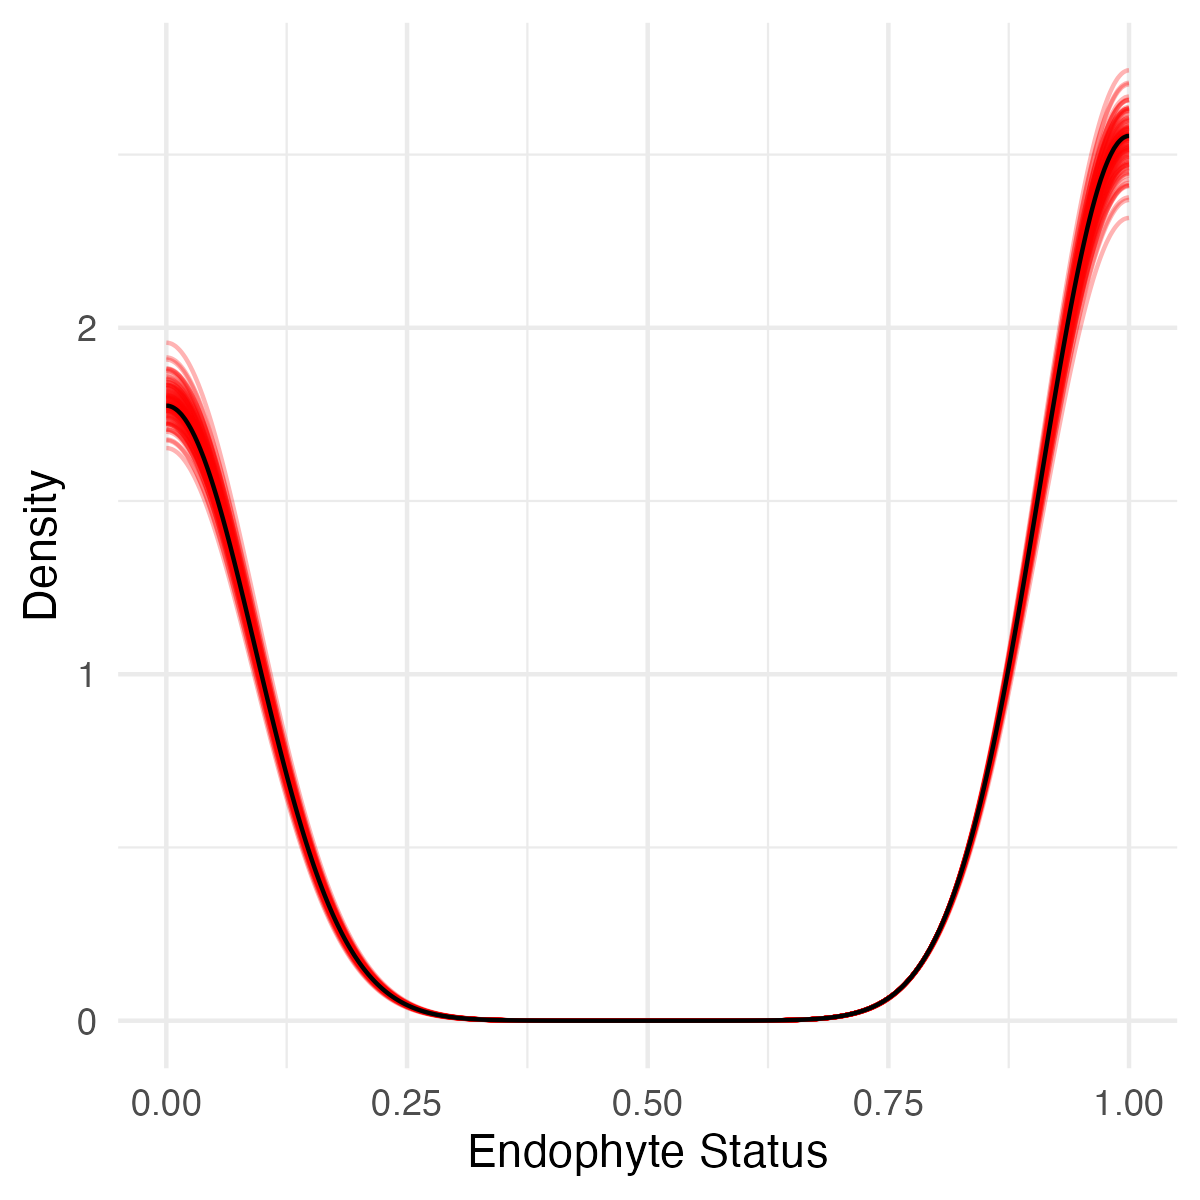
\includegraphics[width = .5\linewidth]{../Plots/overlay_plot.png}
	\caption{\textbf{Consistency between real data and simulated values indicate that the fitted model accurately describes the data}. Graph shows density curves for the observed data (black) along with with 100 simulated datasets (red).}
			\label{fig:overlayplot}
\end{figure}

	
	\begin{figure}[H]
		\centering
		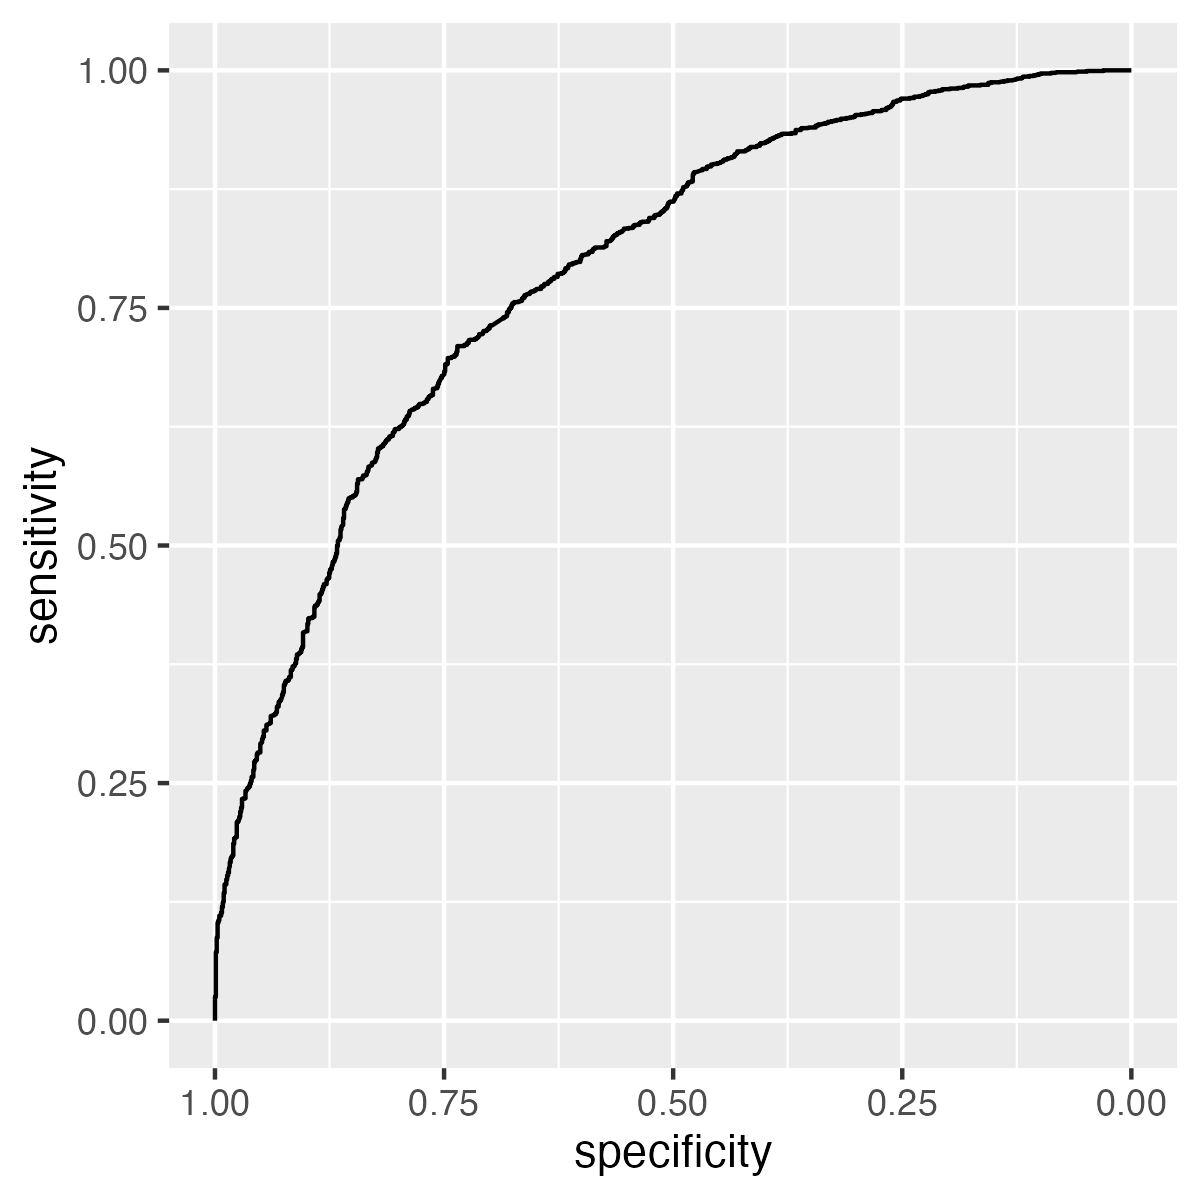
\includegraphics[width = .5\linewidth]{../Plots/ROC_training_plot.png}
		\caption{\textbf{ROC plot showing model performance classifying observations according to endophyte status within the in-sample data.} The curves show adequate model performance for observed data. The AUC value is 0.79.}
				\label{fig:ROCtraining}
	\end{figure}
	
		
	\begin{figure}[H]
		\centering
		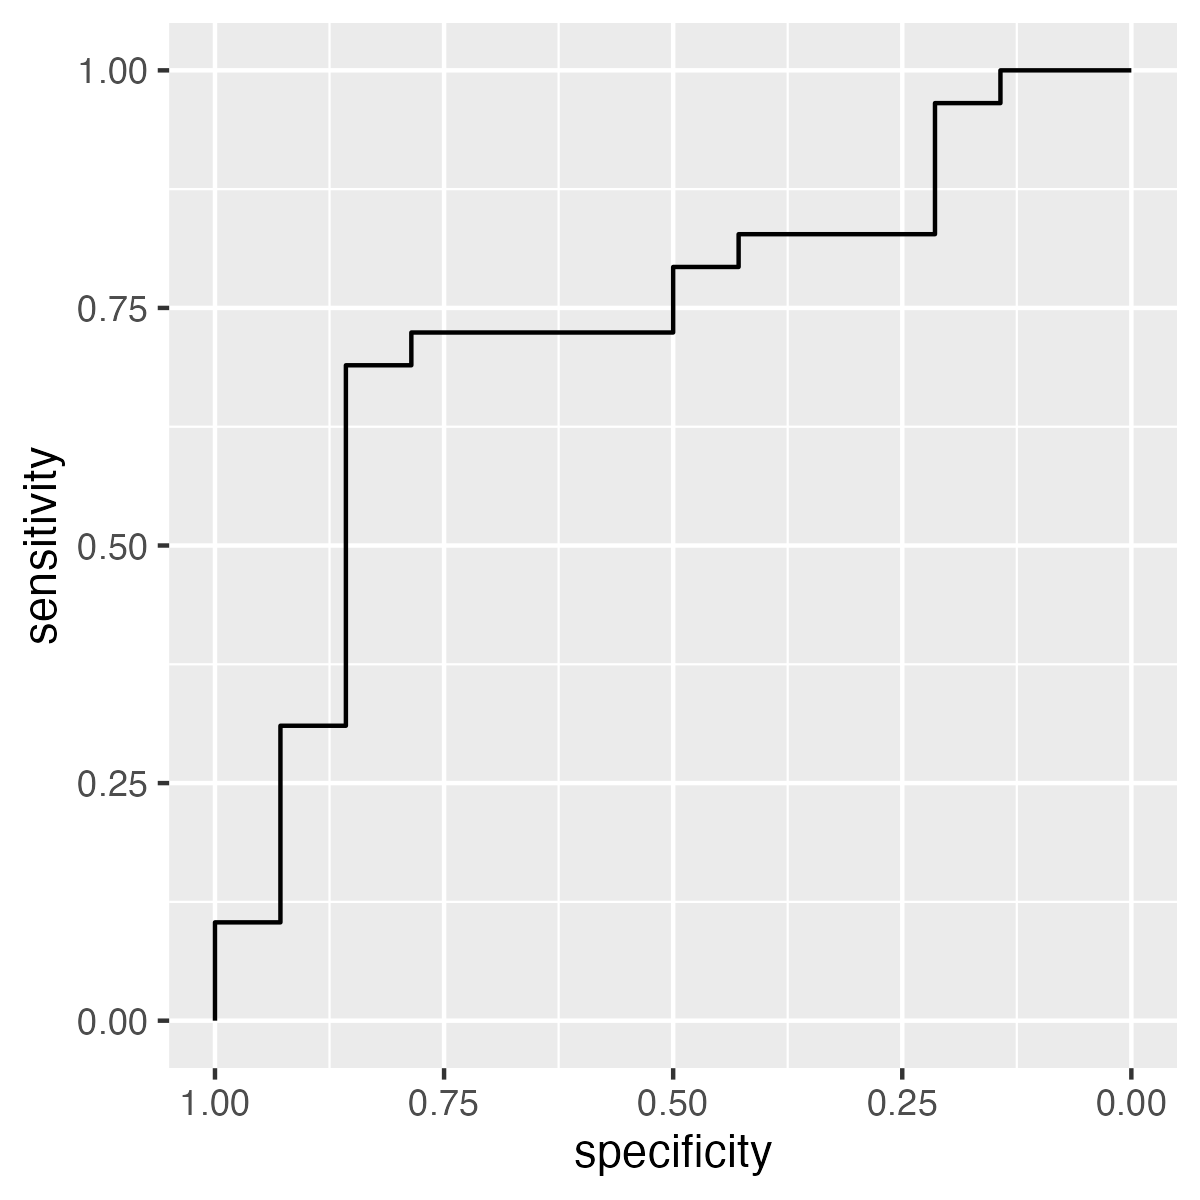
\includegraphics[width = .5\linewidth]{../Plots/ROC_test_plot.png}
		\caption{\textbf{ROC plot showing model performance classifying observations according to endophyte status within the out-of-sample data.} The curves show adequate model performance for test data. The AUC value is 0.77.}
		\label{fig:ROCtest}
	\end{figure}
	
	
\begin{figure}[H]
	\centering
	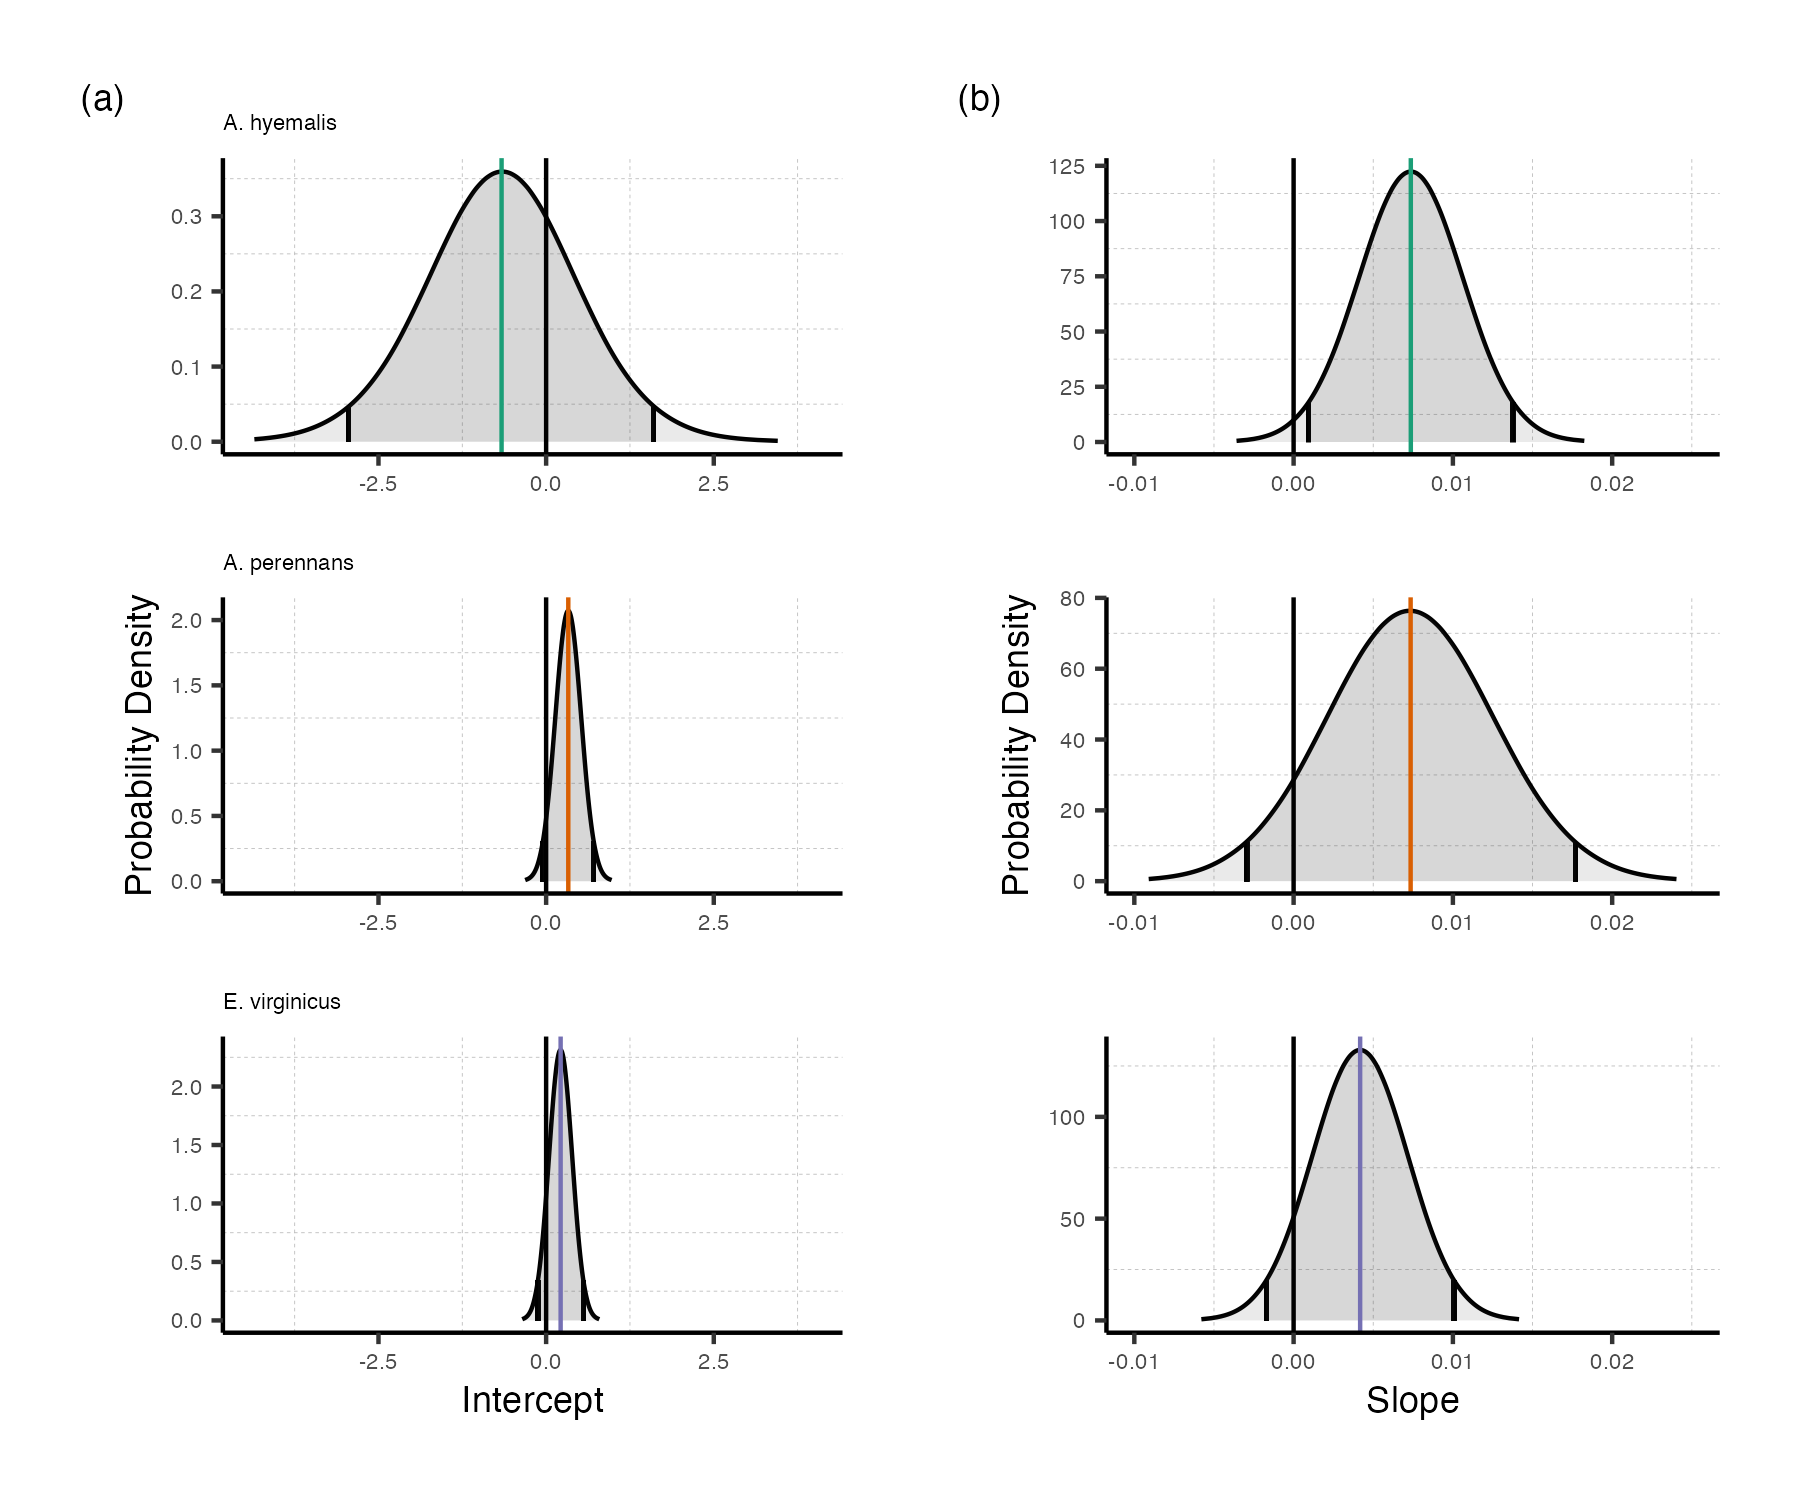
\includegraphics[width = \linewidth]{../Plots/posterior_plot.png}
	\caption[Posterior estimates of parameters describing global temporal trends in endophyte prevalence trends.]{Density curves show the probability density along with mean (colored line) and $95$\% CI (black lines) for the (A) intercept and (B) slope terms, \textbf{A} and \textbf{T} respectively. Colors represent each host species}
	\label{fig:temporal_posterior}
\end{figure}


\begin{figure}[H]
	\centering
	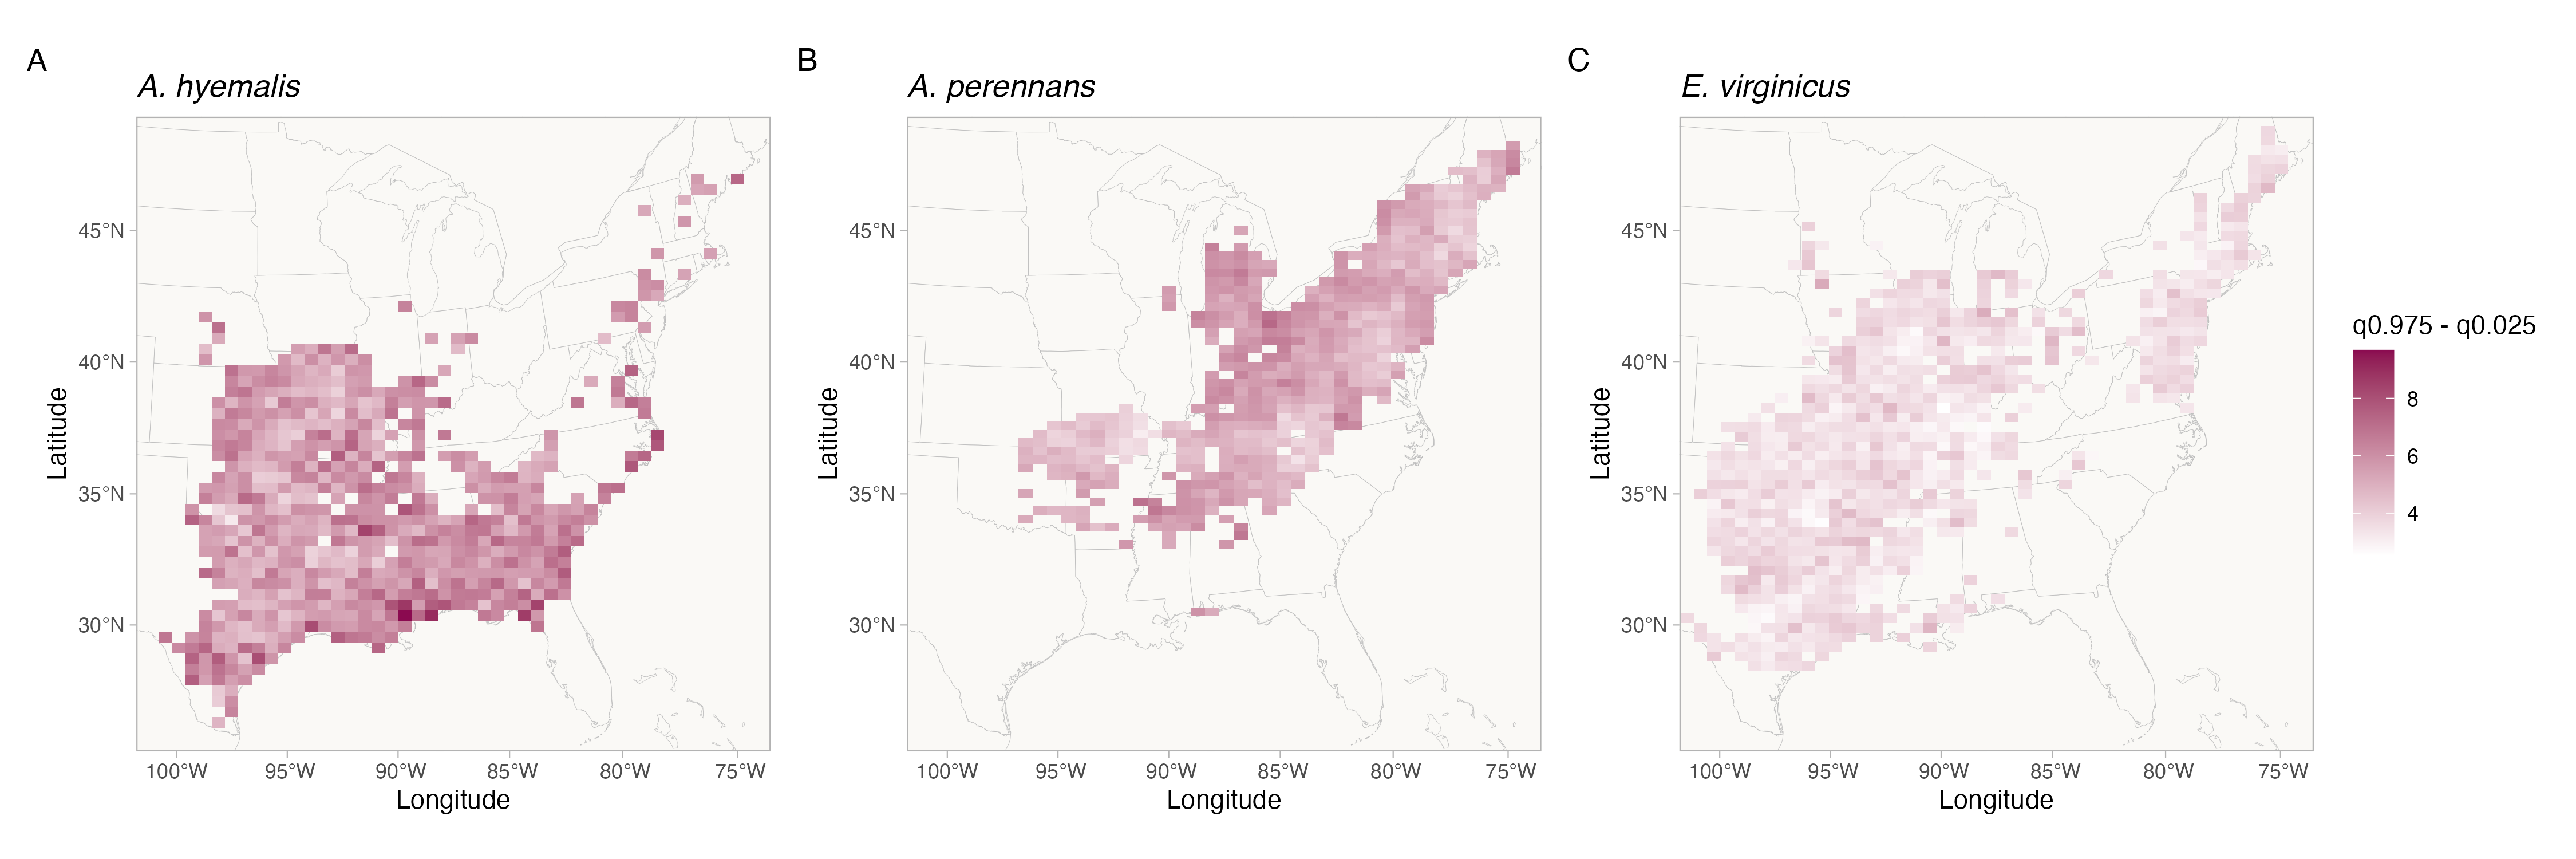
\includegraphics[width = \linewidth]{../Plots/svc_time_map_CI.png}
	\caption[Uncertainty in spatially-varying trends representing change in endophyte prevalence for each host species.]{Shading represents the range of the 95\% posterior credible interval for spatially varying slopes, $\tau$.}
	\label{fig:svc_time_map_CI}
\end{figure}


\begin{figure}[H]
	\centering
	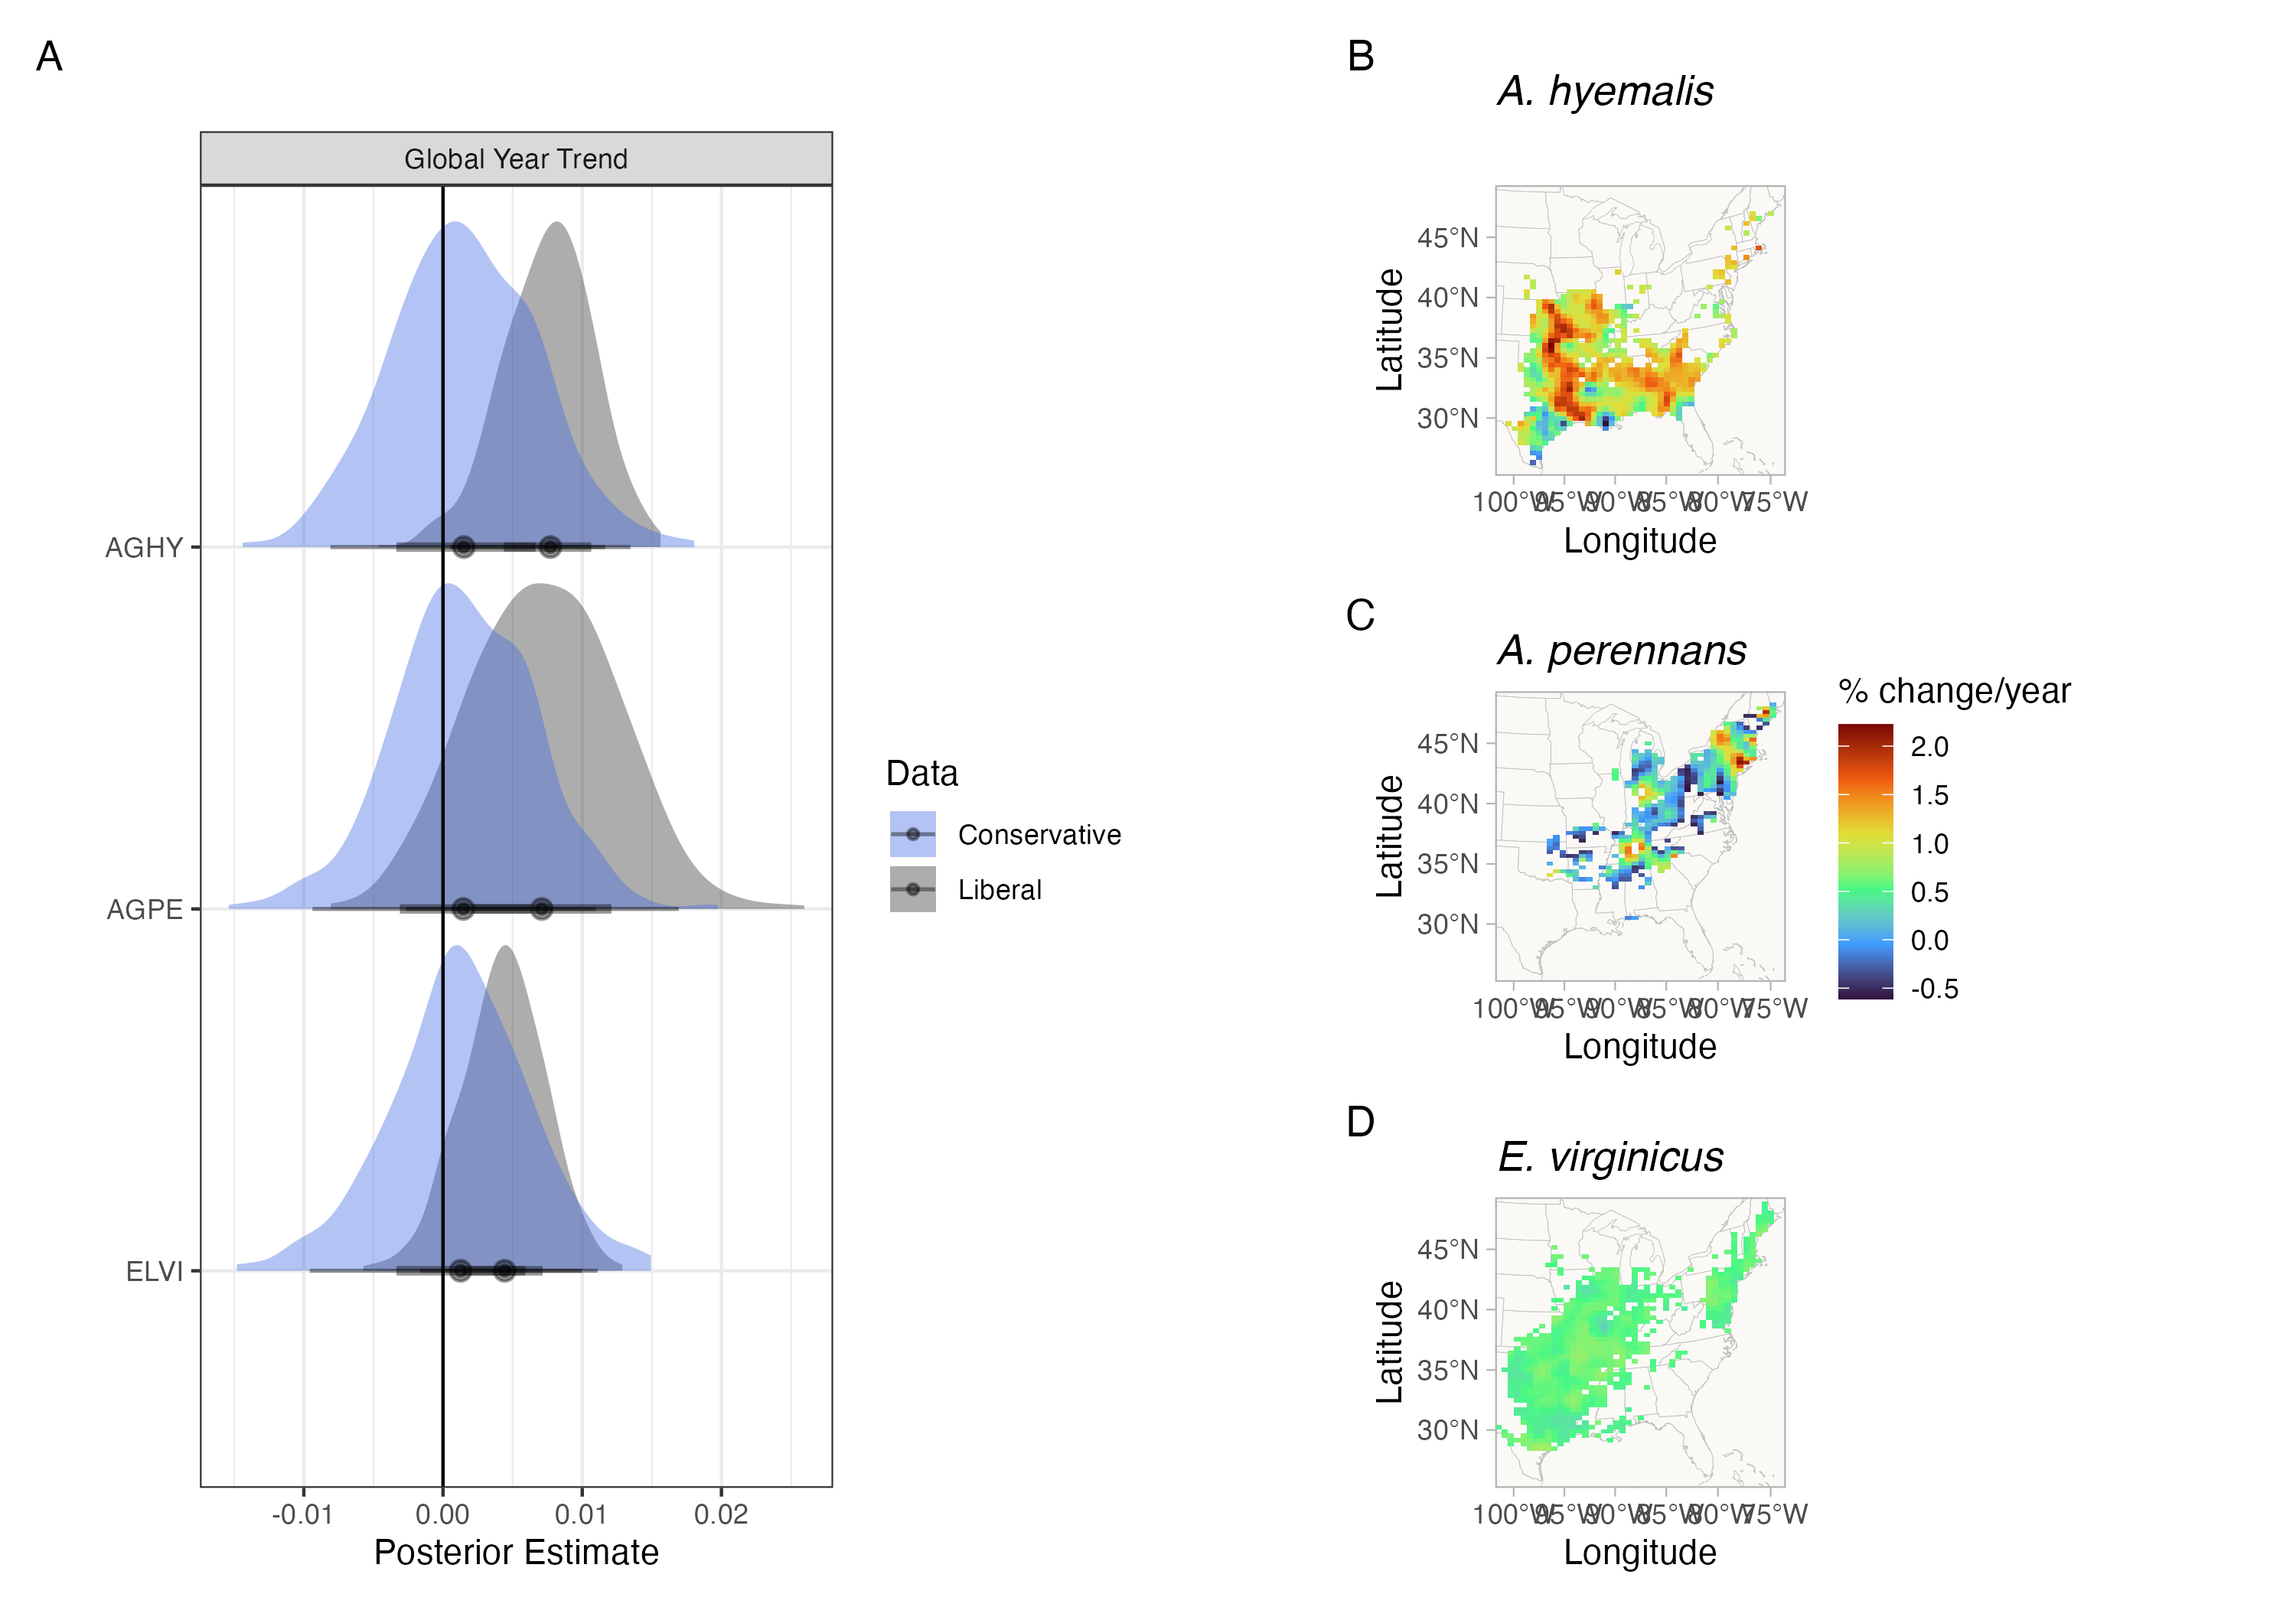
\includegraphics[width = \linewidth]{../Plots/conservative_comparison_plot.png}
	\caption{Comparison of liberal versus conservative endophyte scores on modeled outcomes. (A) Posterior estimates of global temporal trend for models fit to liberal scores (grey) and to conservative scores (blue). Maps show the spatially varying temporal trend estimates from model fit to conservative scores for (B) \emph{A. hyemalis}, (C) \emph{A. perennans}, and (D) \emph{E. virginicus}. Note that the color scale differs between this visualization and Fig. \ref{fig:svc_time_map}.}
	\label{fig:conservative_scores_plot}
\end{figure}


\begin{figure}[H]
	\centering
	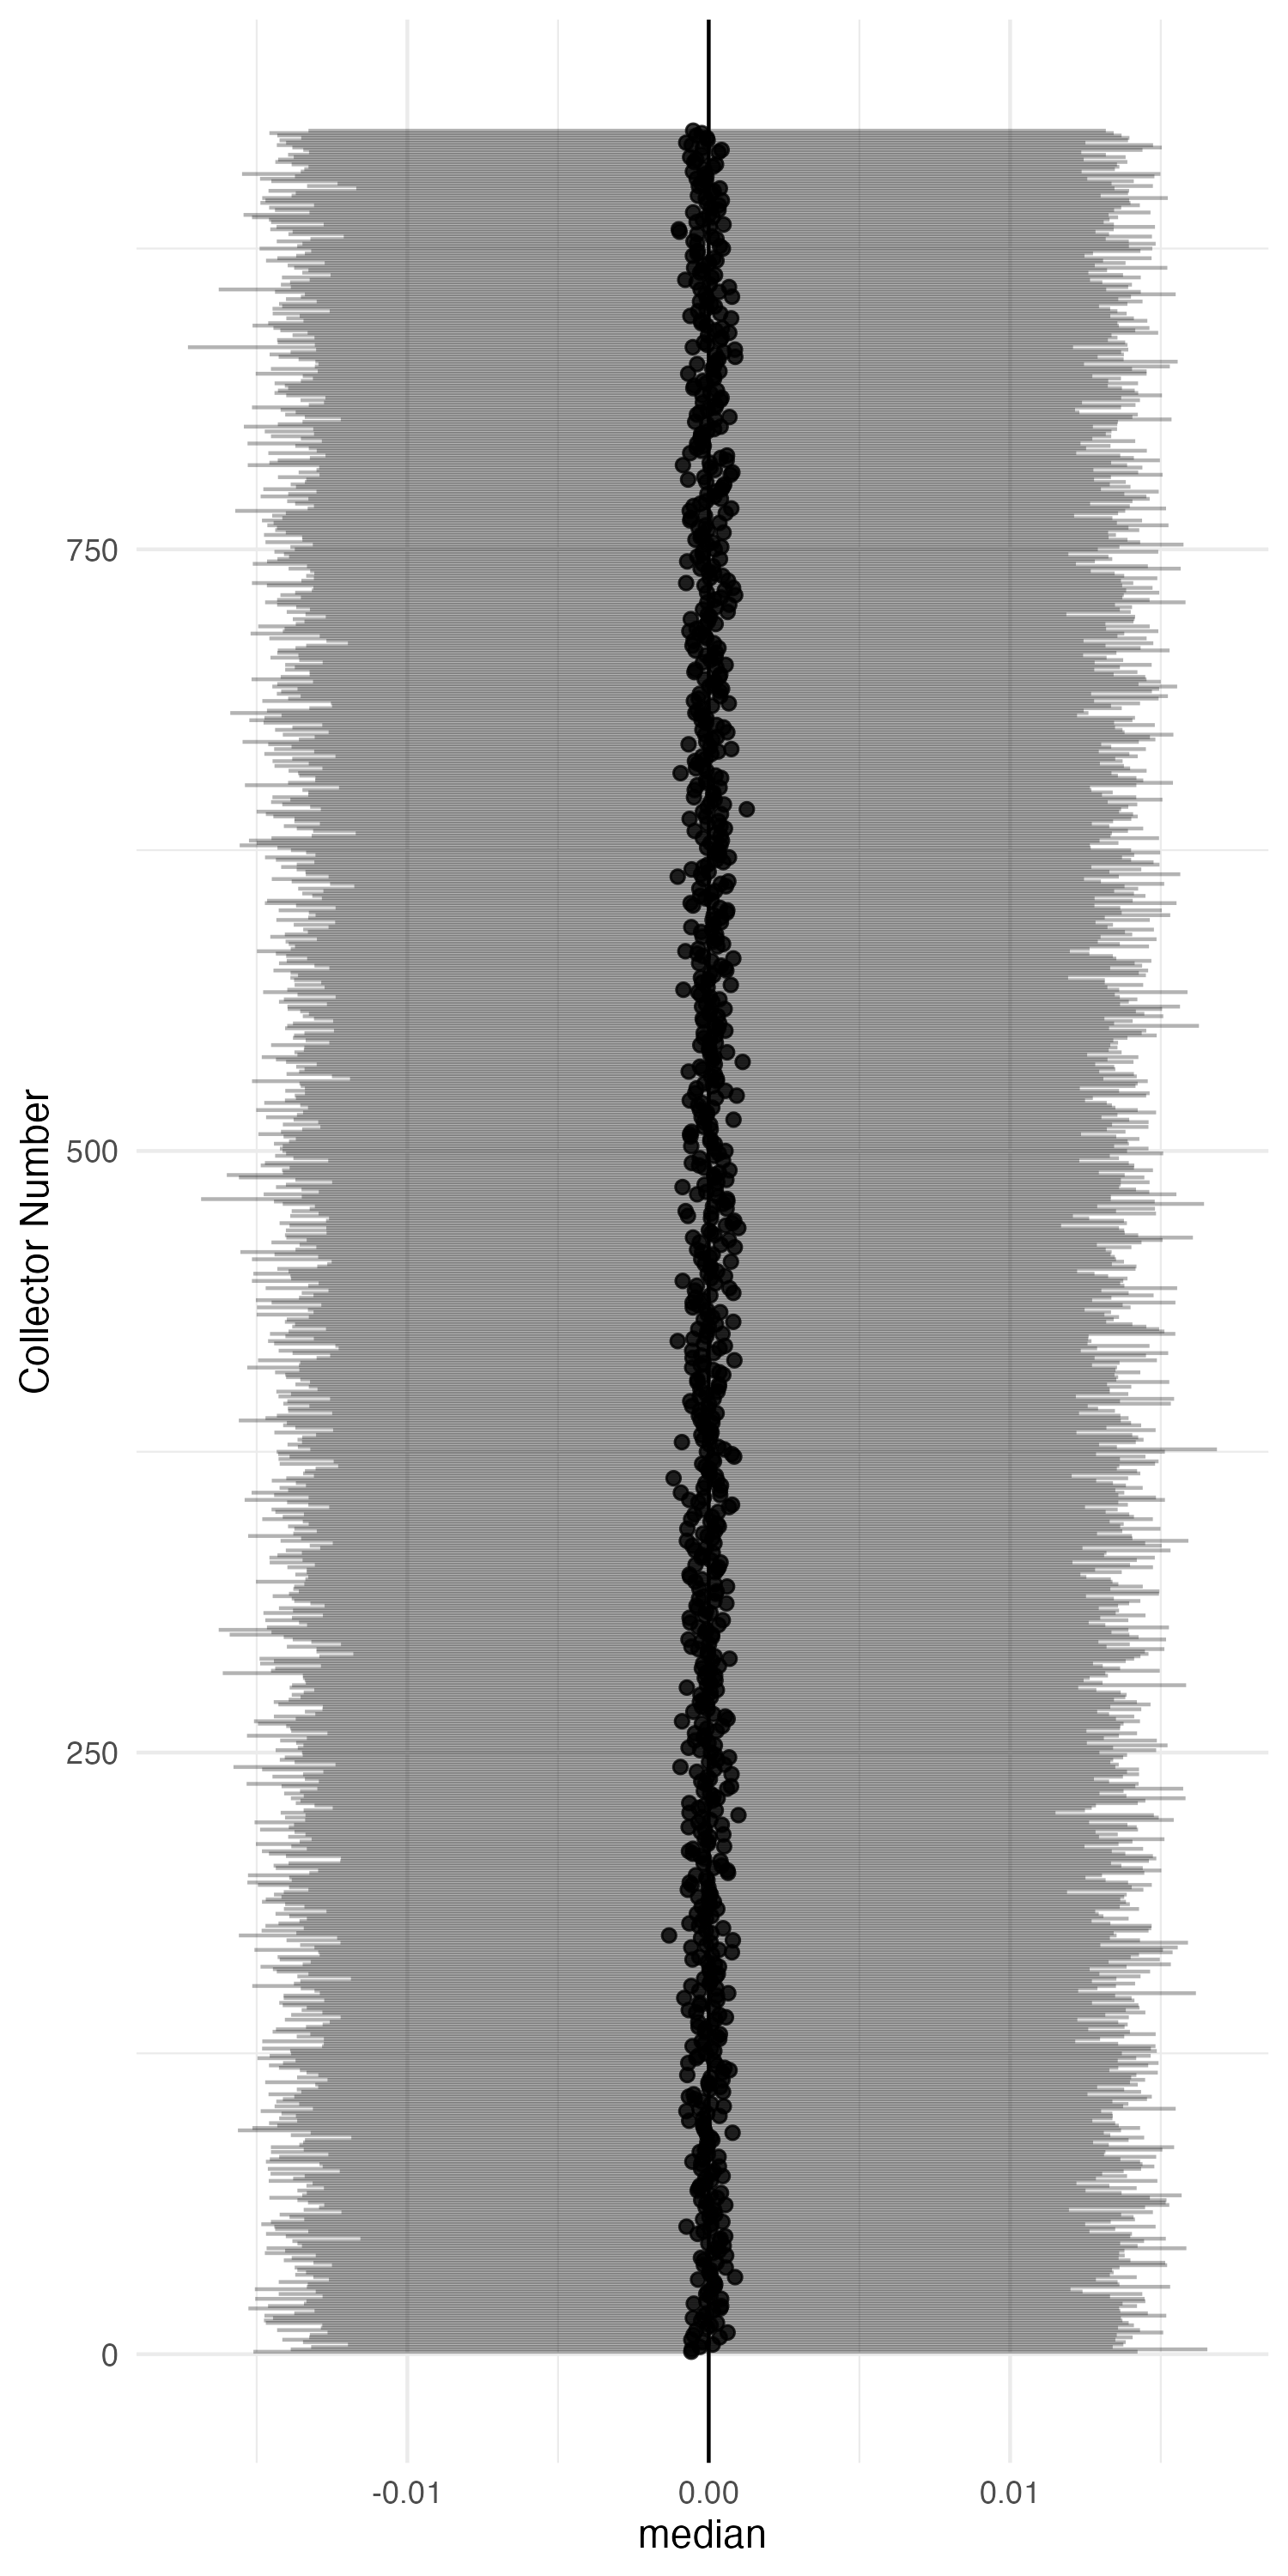
\includegraphics[width = .6\linewidth]{../Plots/collector_posterior.png}
	\caption{\textbf{Posterior estimates of collector random effects.} Points show posterior median along with 95\% CI for each of $924$ individual collectors.}
		\label{fig:collector_fx}
\end{figure}


\begin{figure}[H]
	\centering
	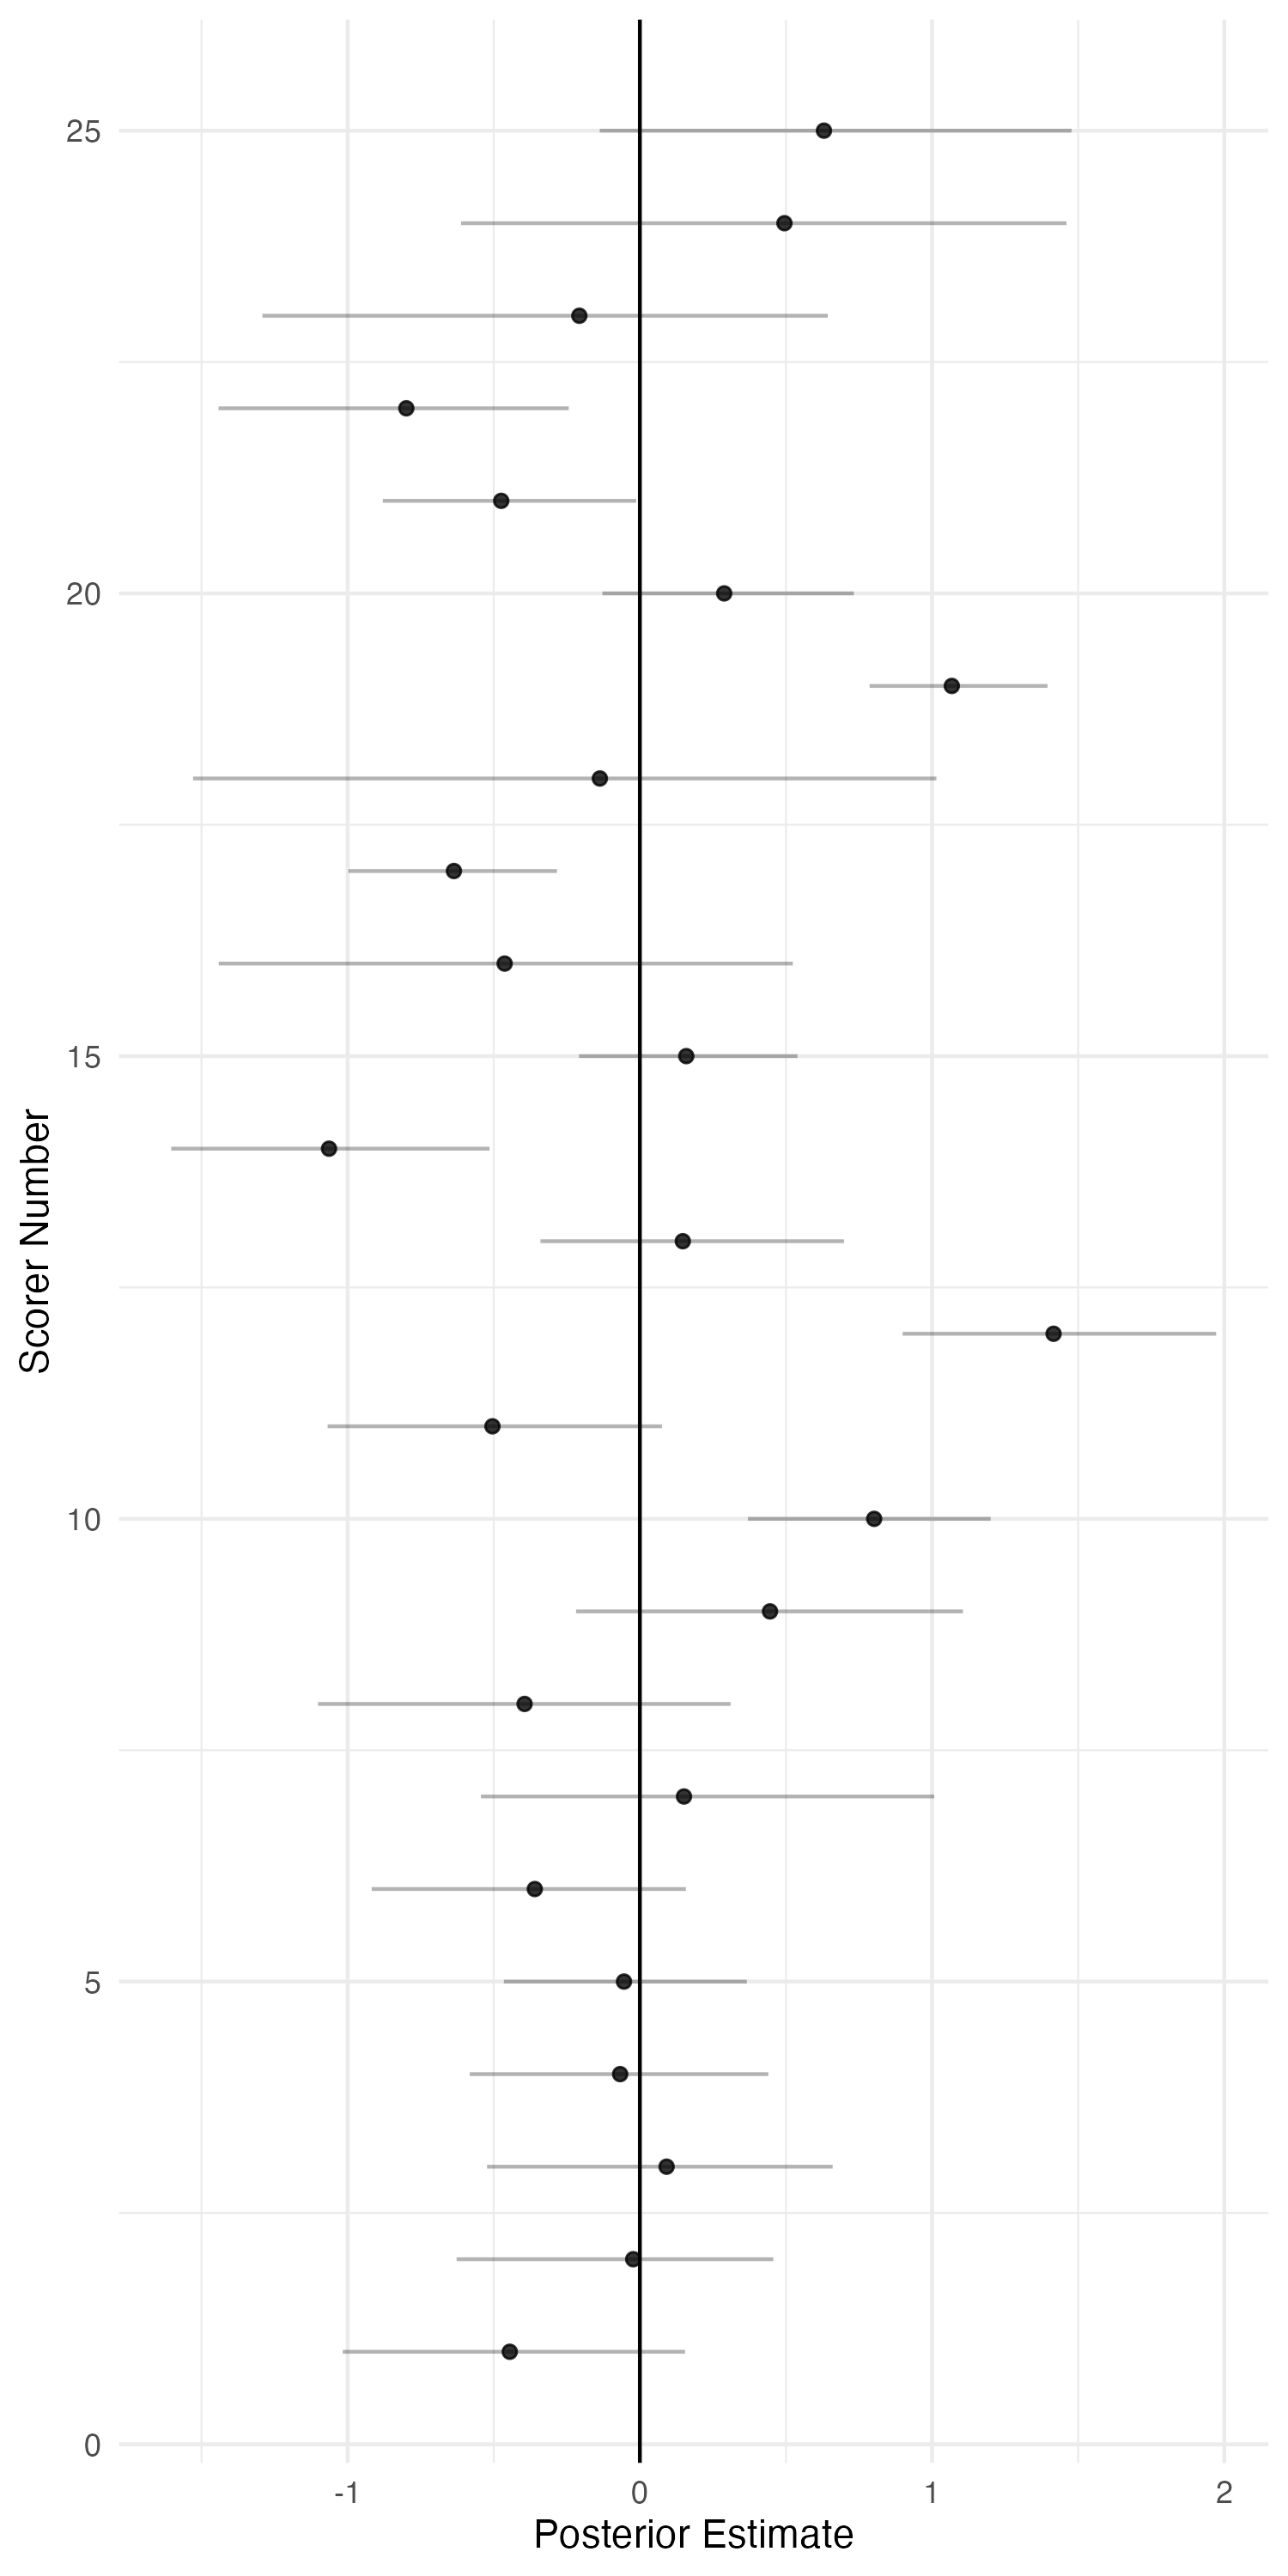
\includegraphics[width = .6\linewidth]{../Plots/scorer_posterior.png}
	\caption{\textbf{Posterior estimates of scorer random effects.} Points show posterior median along with 95\% CI for each of $25$ individual collectors.}
	\label{fig:scorer_fx}
\end{figure}


\begin{figure}[H]
	\centering
	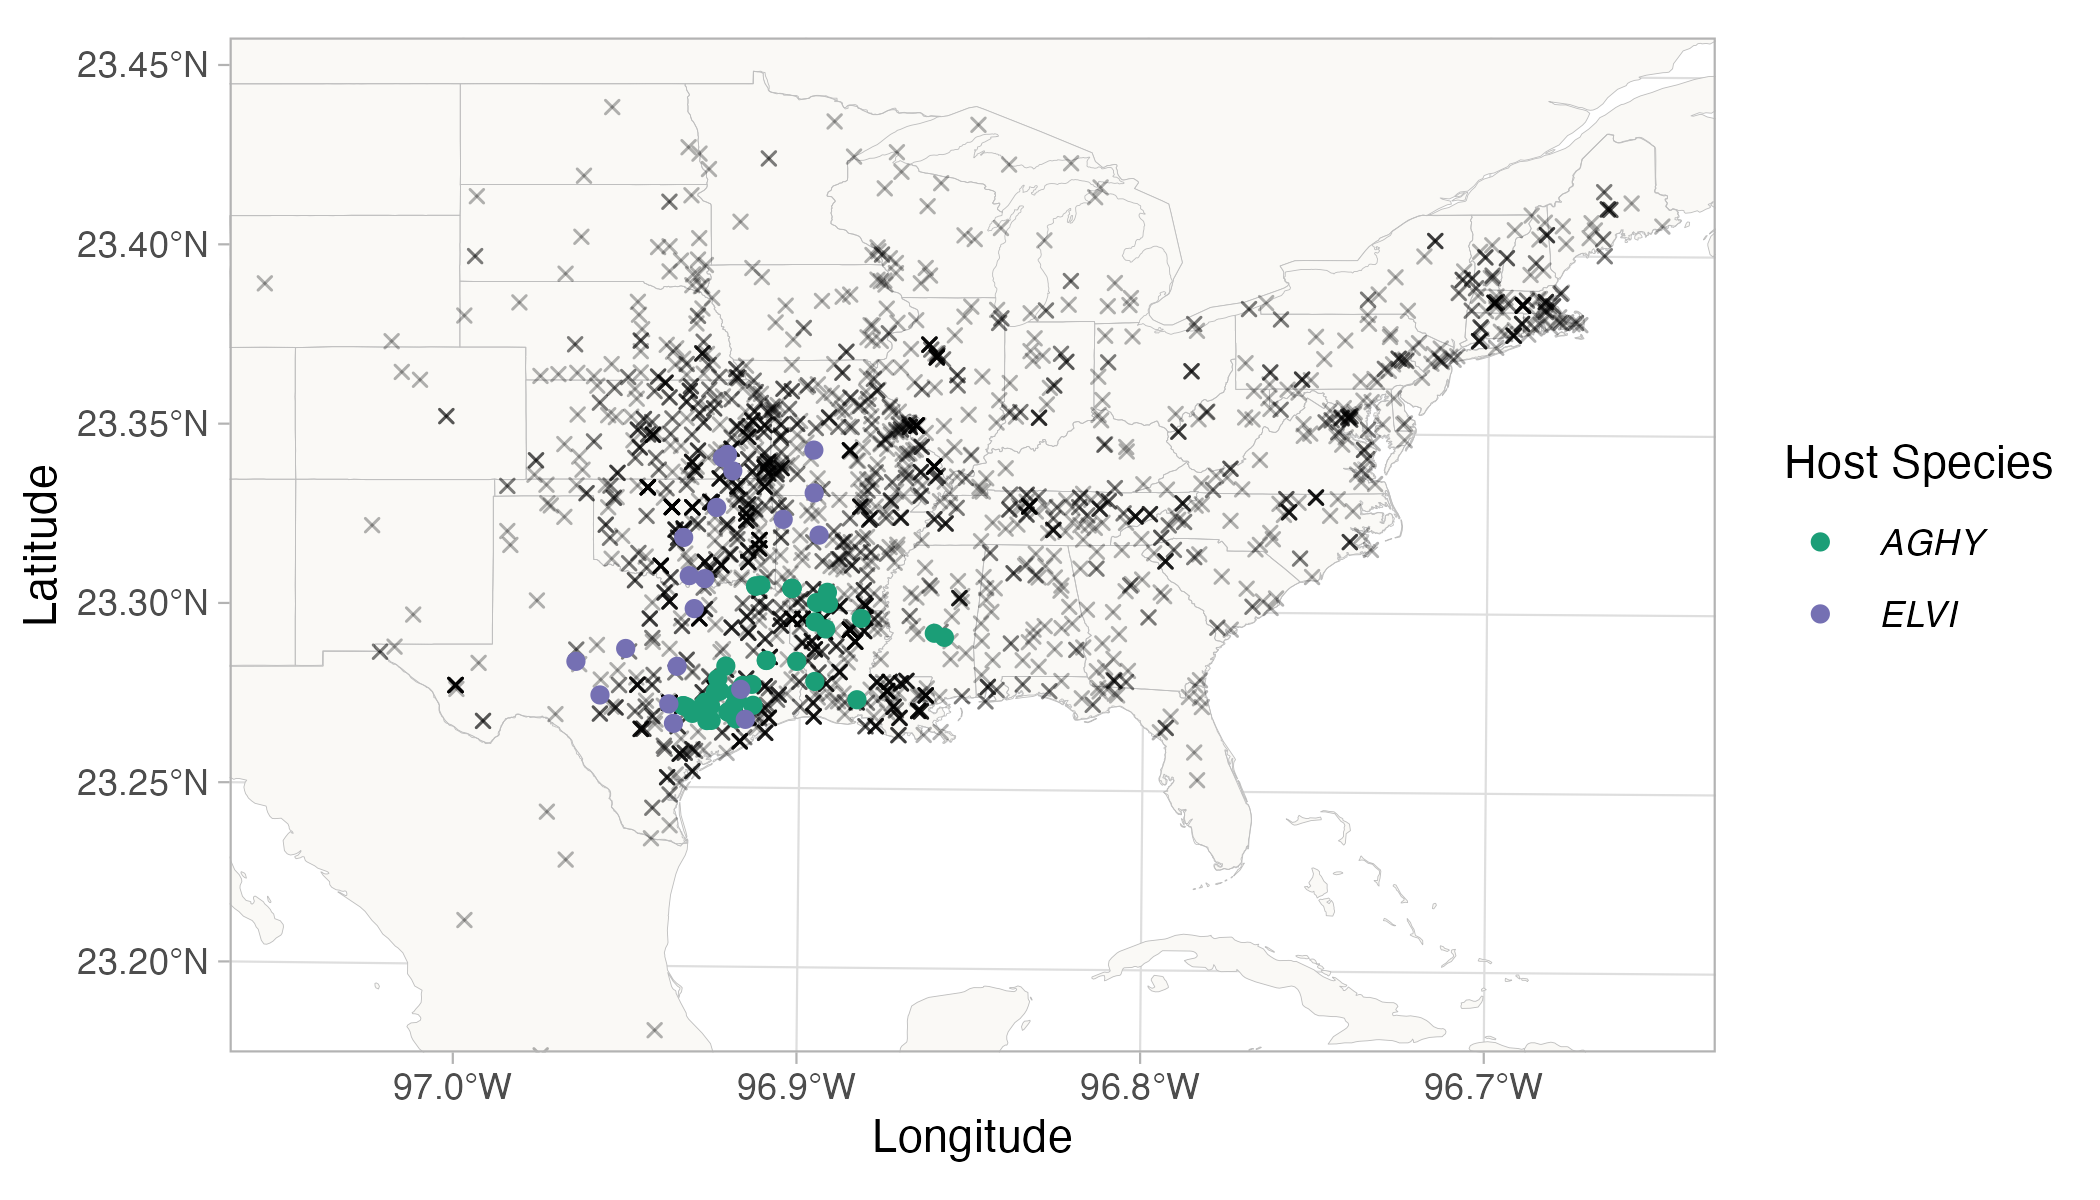
\includegraphics[width = \linewidth]{../Plots/contemp_surveys_map.png}
	\caption{\textbf{Locations of contemporary surveys of endophytes in \emph{A. hyemalis} used as "test" data (red points), relative to the historical collection data (black crosses).}}
	\label{fig:contempsurveysmap}
\end{figure}

	\begin{figure}[H]
	\centering
	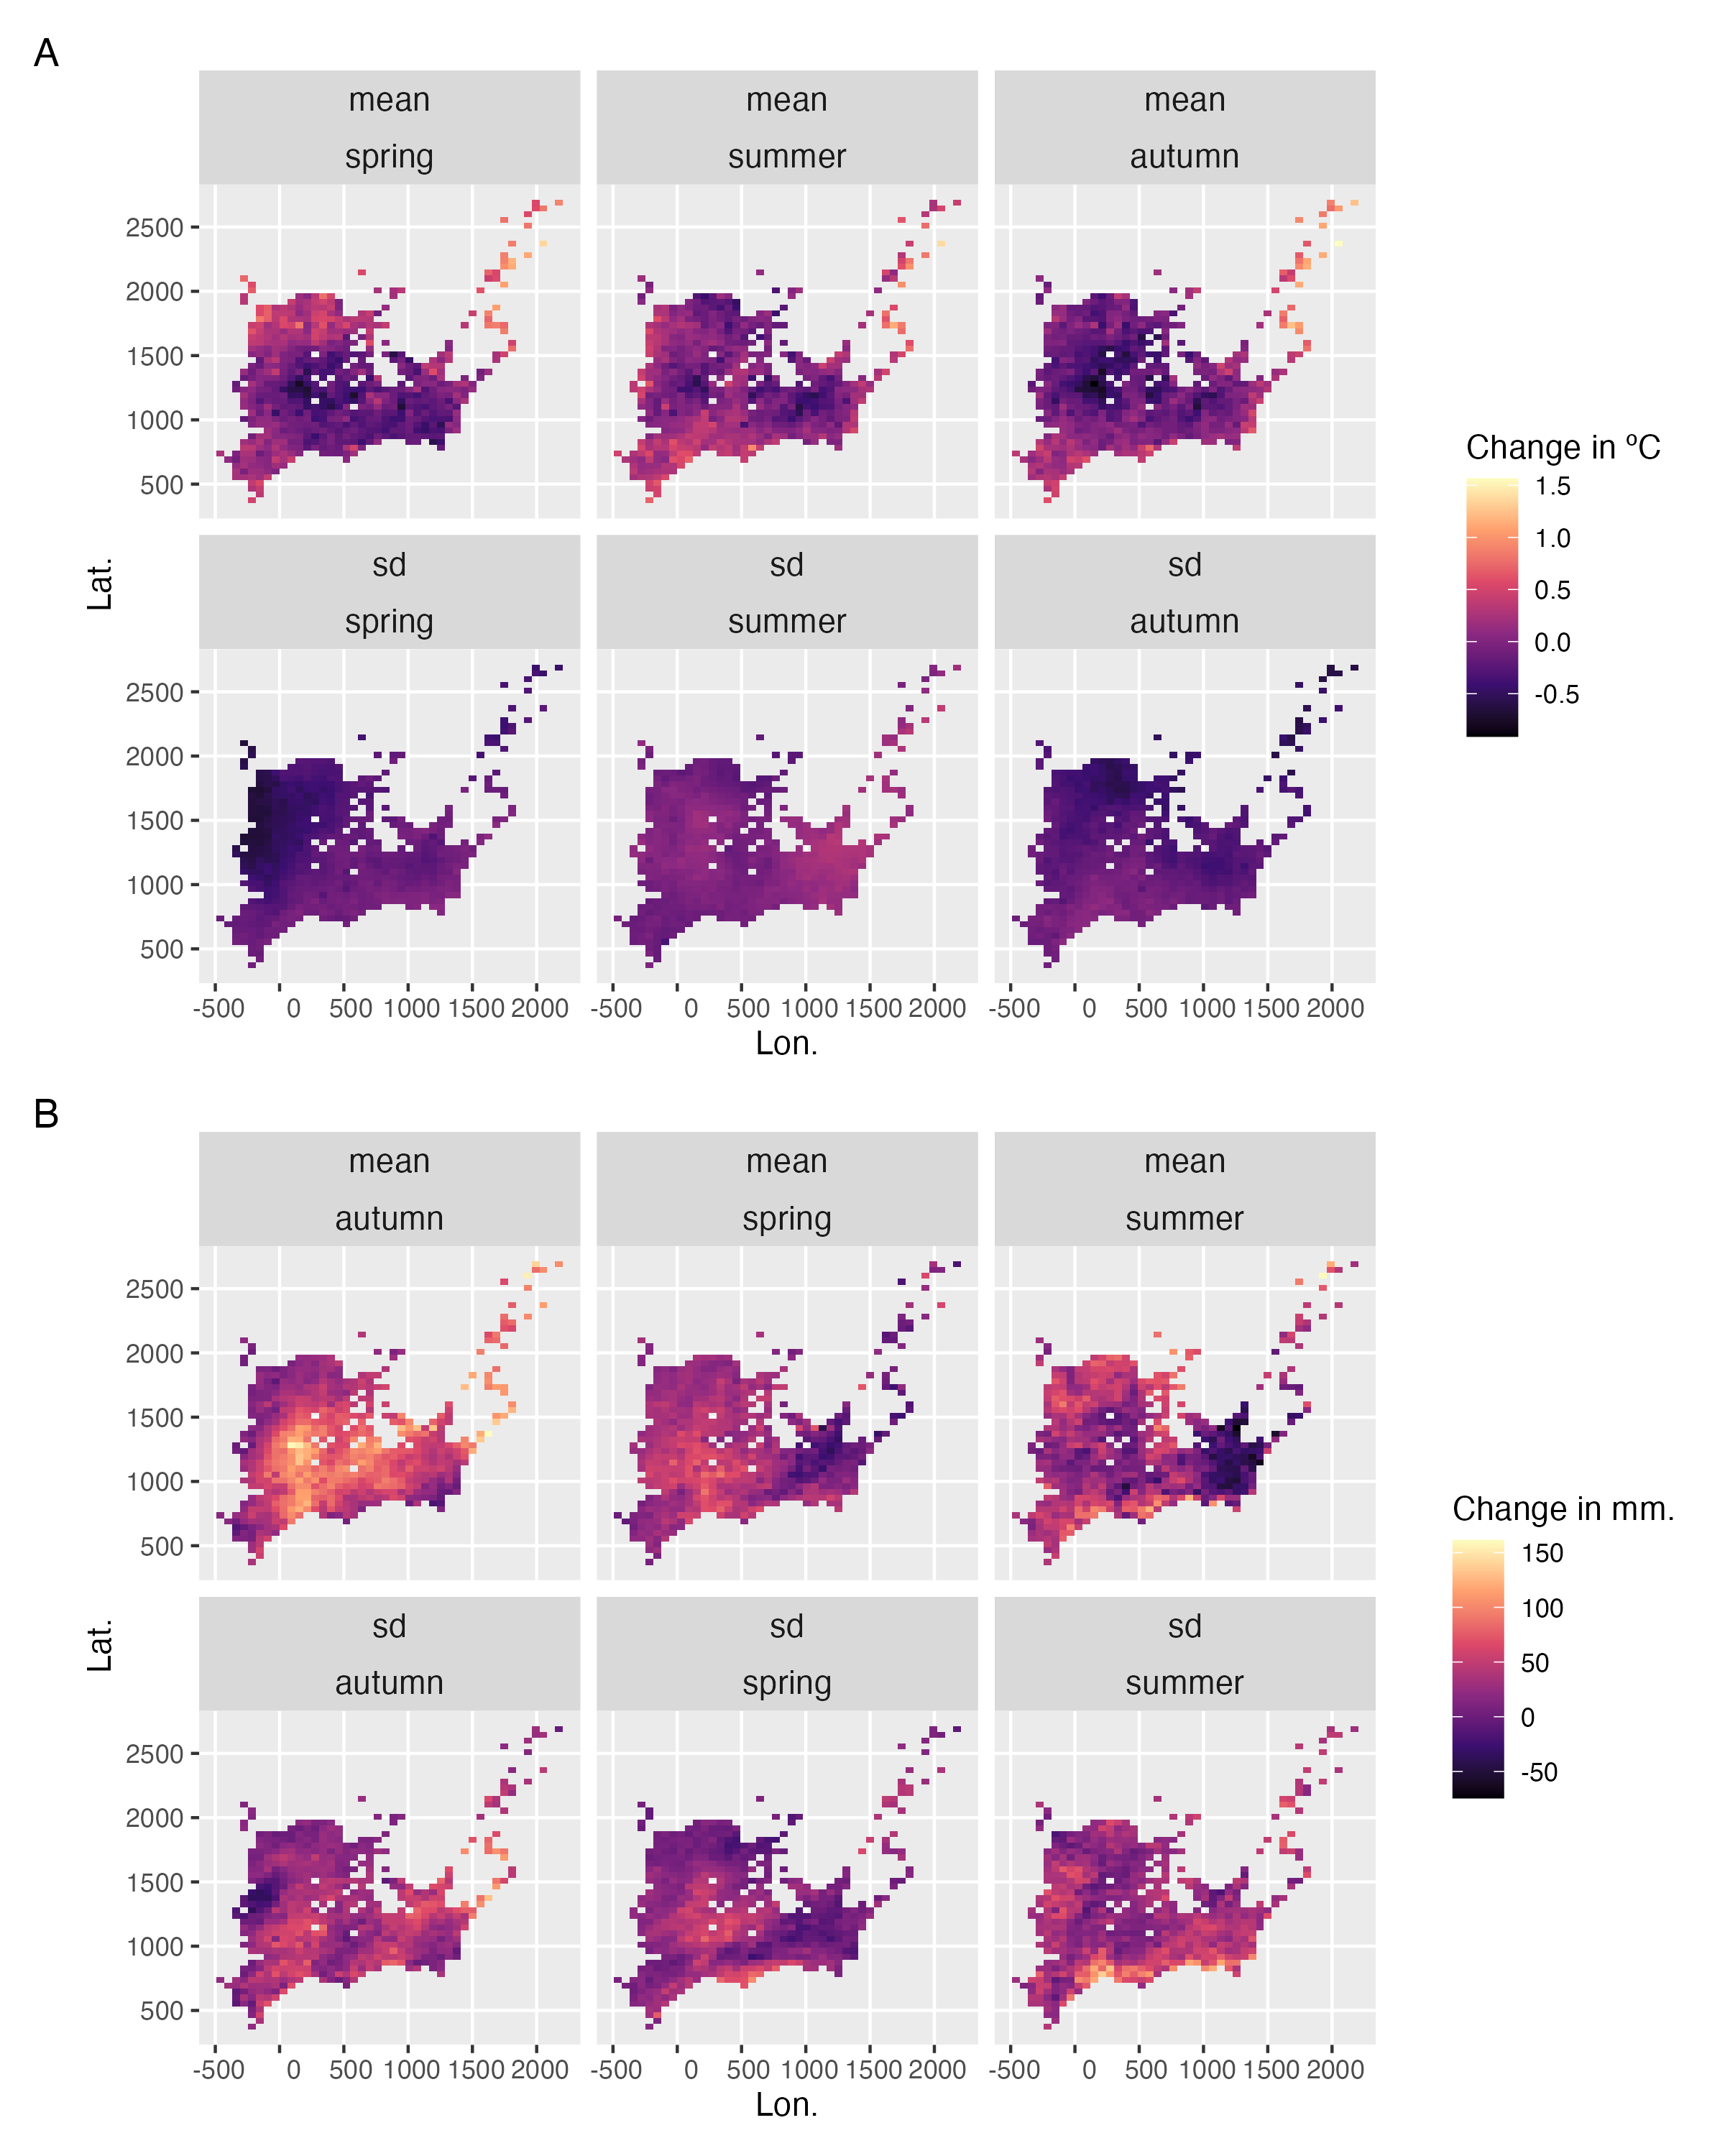
\includegraphics[width = .8\linewidth]{../Plots/AGHY_climate_change_plot.png}
	\caption{\textbf{Change in seasonal climate variables between the periods 1895-1925 and 1990-2020.} Color represents change in (A) seasonal temperature and (B) seasonal precipitation. Maps show pixels covering the modeled distribution of \emph{A. hyemalis} used in post-hoc climate correlation analysis.}
	\label{fig:AGHY_climate_covariates}
\end{figure}

\begin{figure}[H]
	\centering
	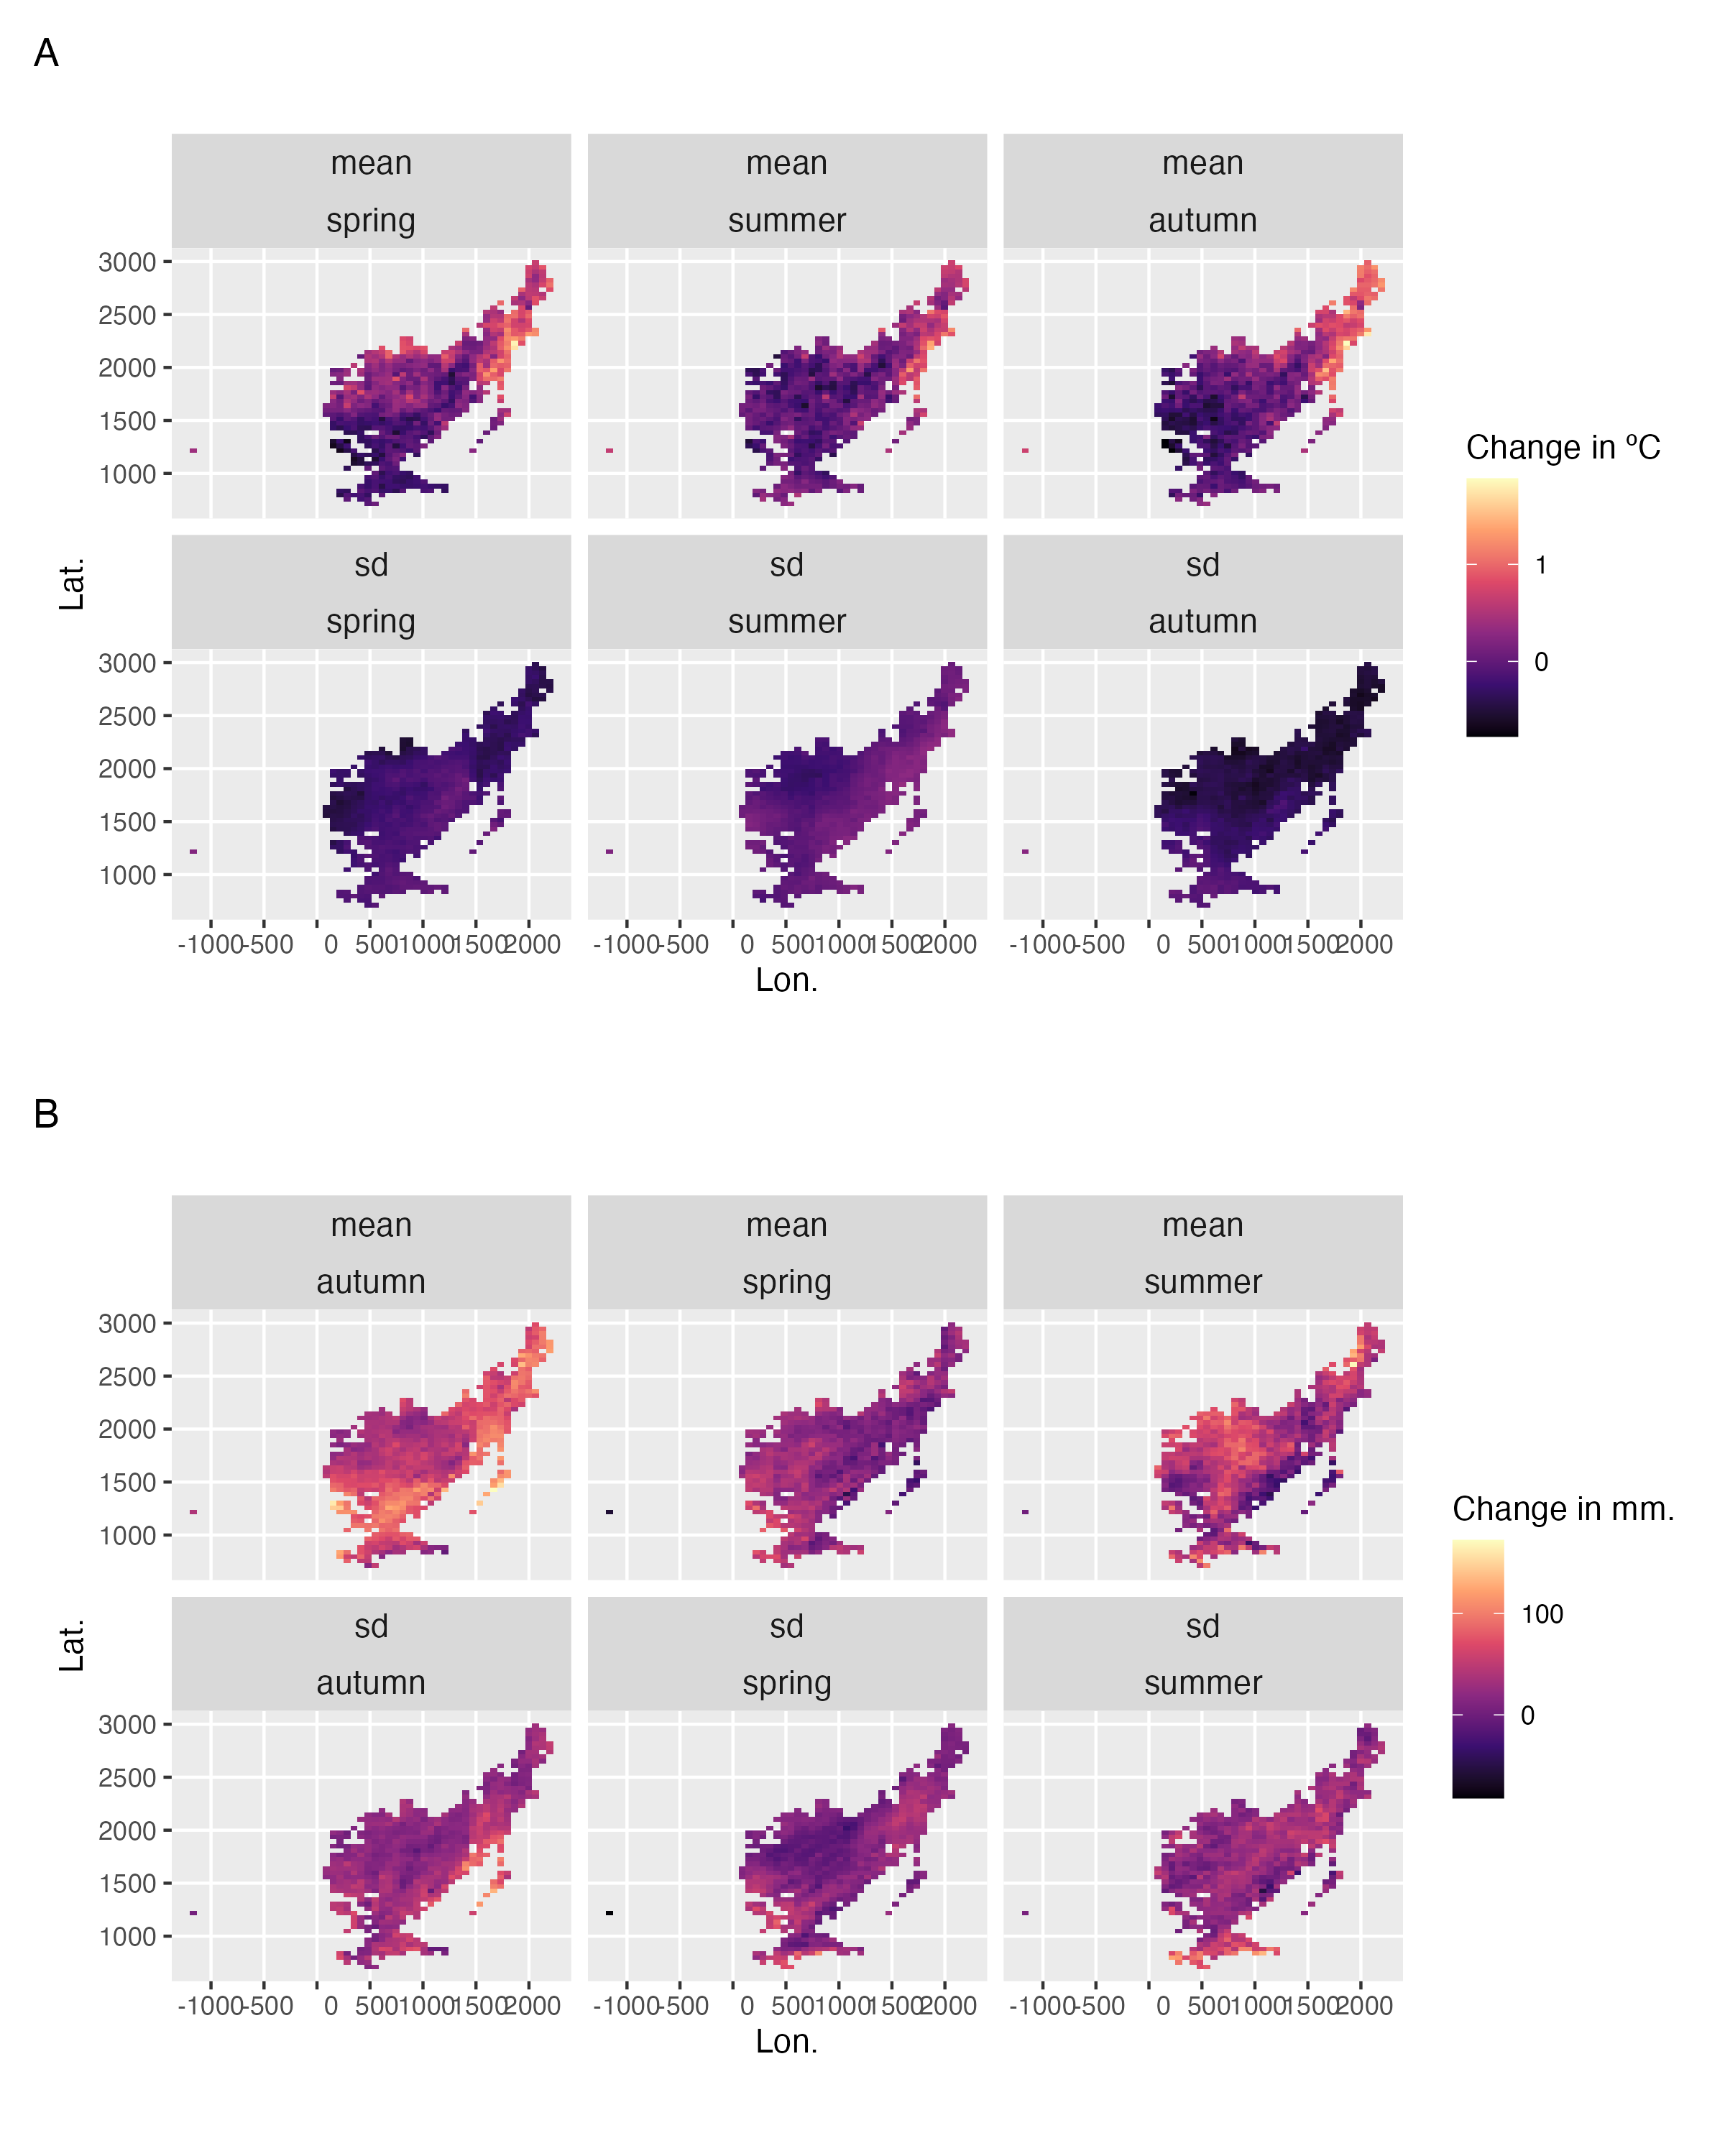
\includegraphics[width = .8\linewidth]{../Plots/AGPE_climate_change_plot.png}
	\caption{\textbf{Change in seasonal climate variables between the periods 1895-1925 and 1990-2020.} Color represents change in (A) seasonal temperature and (B) seasonal precipitation. Maps show pixels covering the modeled distribution of \emph{A. perennans} used in post-hoc climate correlation analysis.}
	\label{fig:AGPE_climate_covariates}
\end{figure}

\begin{figure}[H]
	\centering
	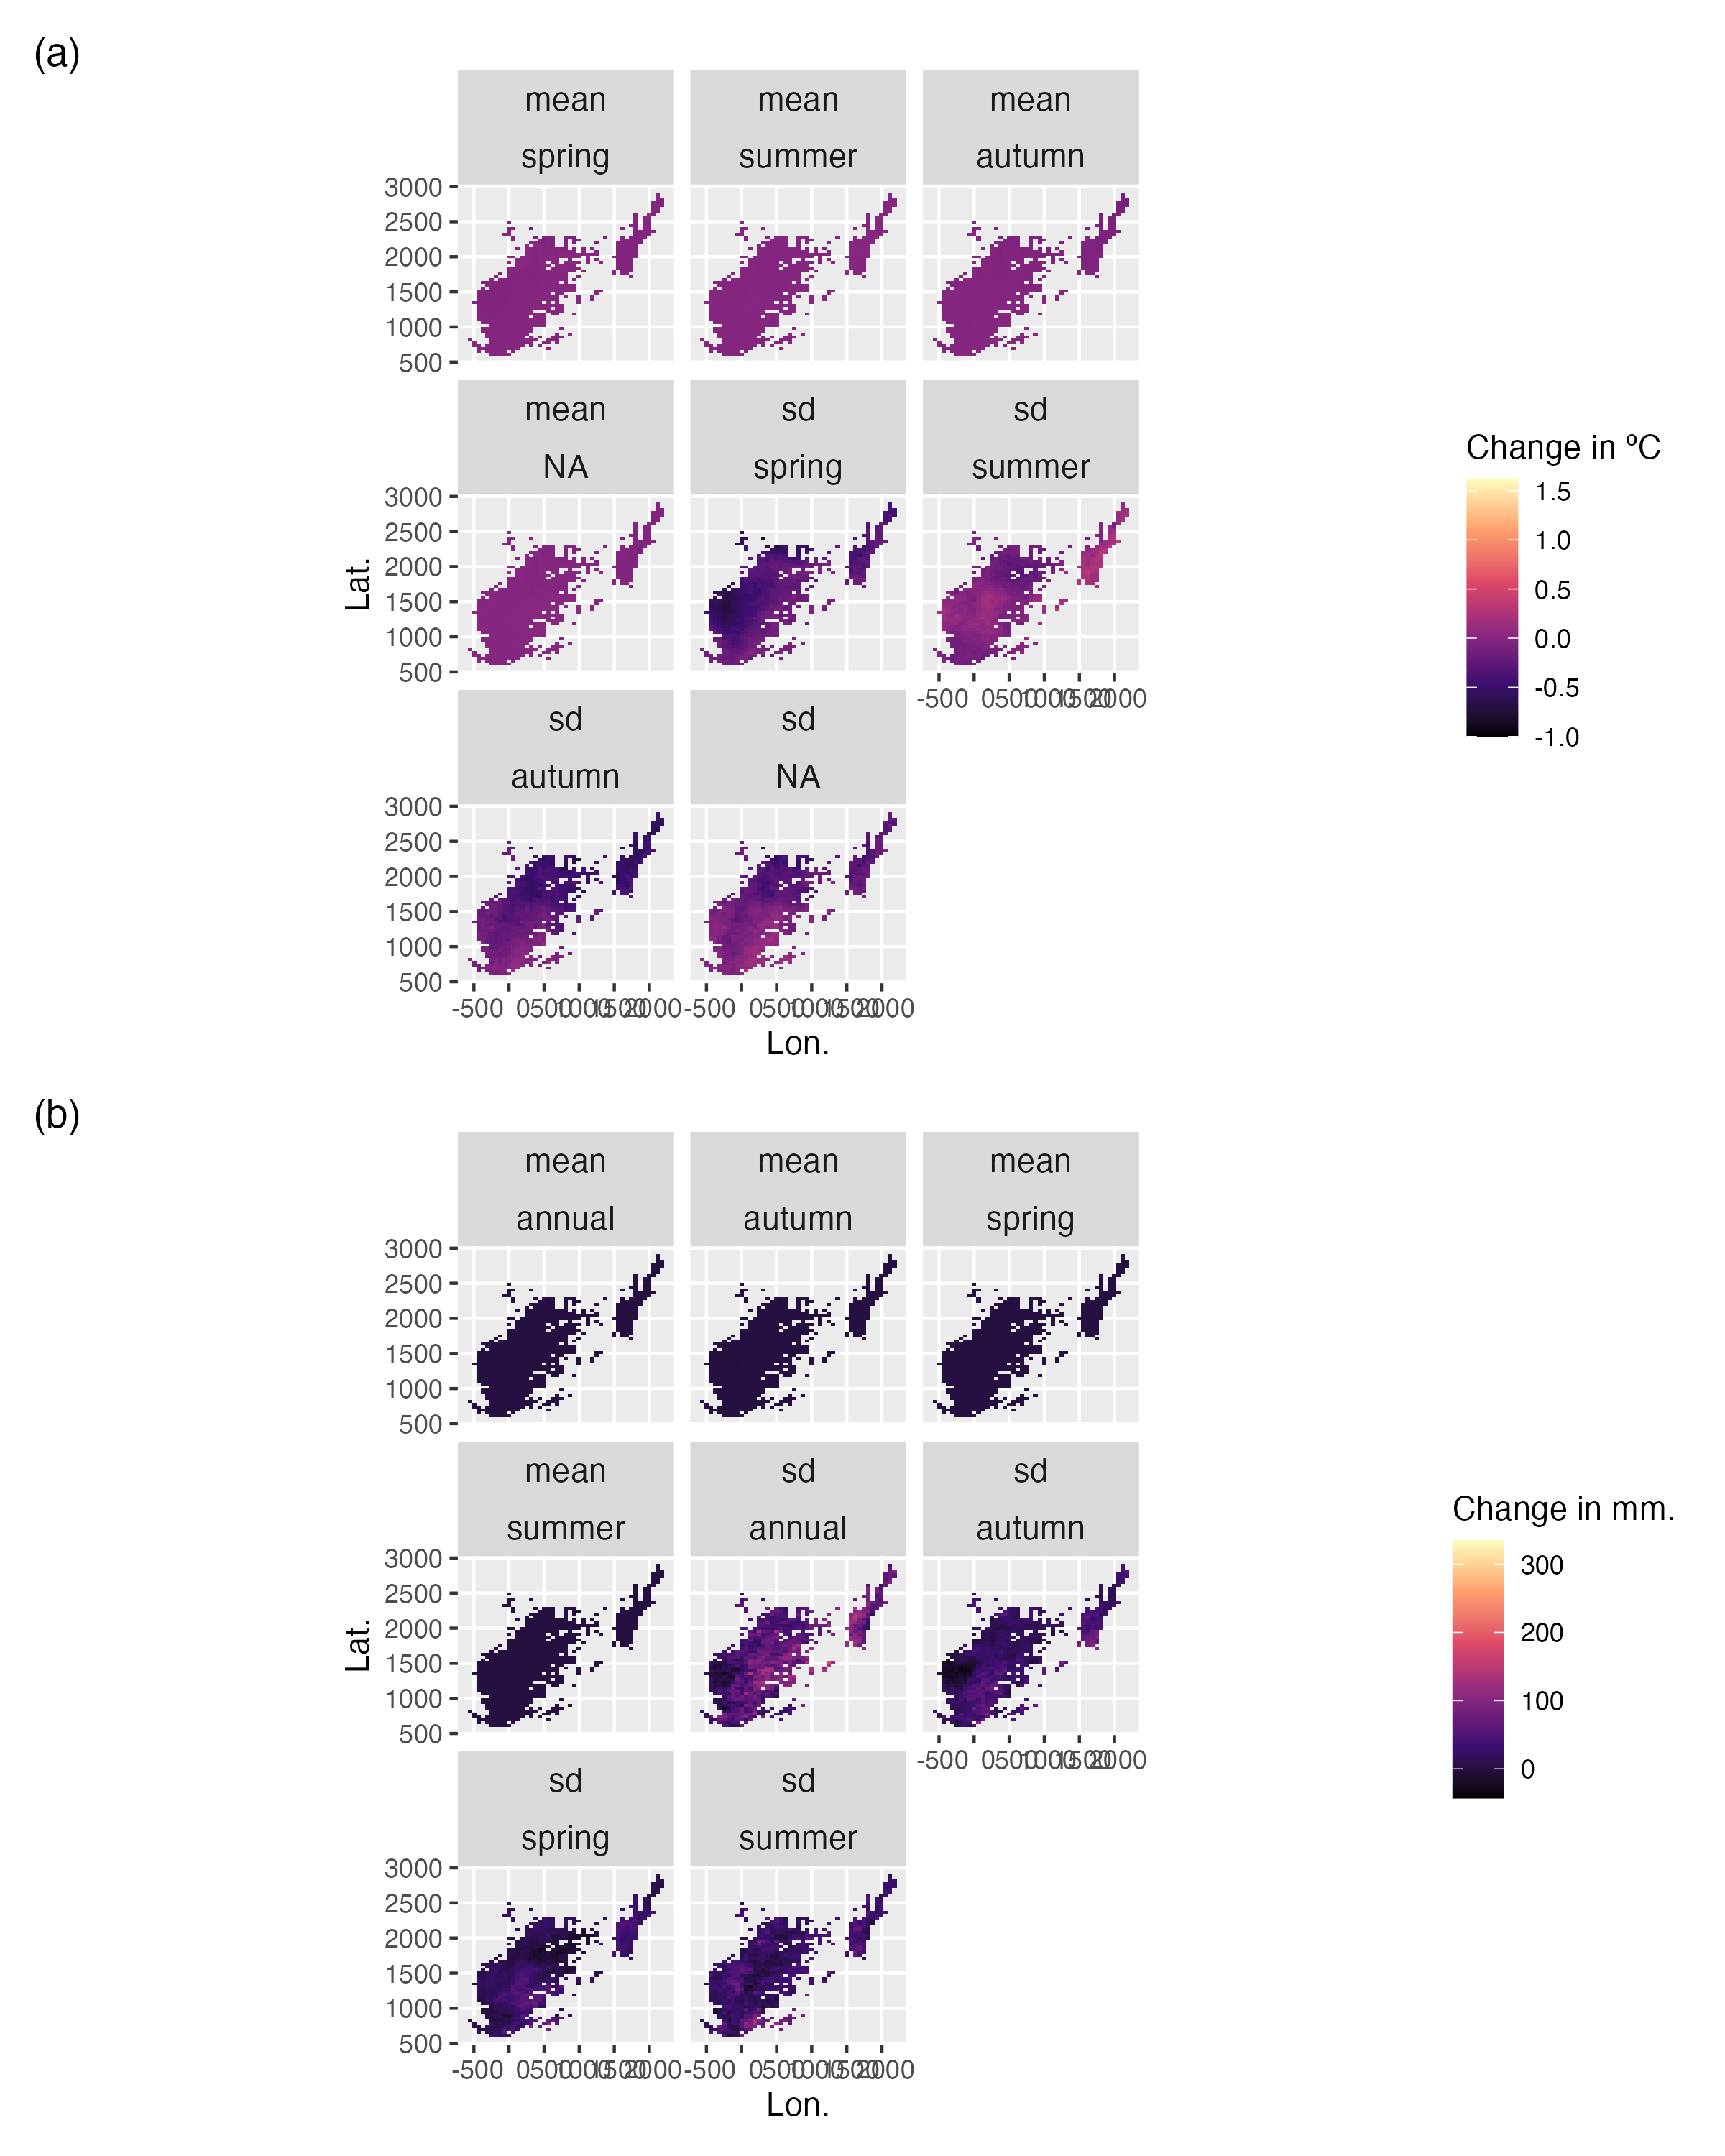
\includegraphics[width = .8\linewidth]{../Plots/ELVI_climate_change_plot.png}
	\caption{\textbf{Change in seasonal climate variables between the periods 1895-1925 and 1990-2020.} Color represents change in (A) seasonal temperature and (B) seasonal precipitation. Maps show pixels covering the modeled distribution of \emph{E. virginicus} used in post-hoc climate correlation analysis.}
	\label{fig:ELVI_climate_covariates}
\end{figure}


	
	\begin{table}[h]
		\caption{Summary of herbarium samples across collections}
		\label{table:herbaria}
		\centering
		\begin{tabular}{llll}\hline
			Herbarium Collection        & AGHY        & AGPE      &      ELVI\\ \hline
			Botanical Research Institute of Texas &   350   &    190&    198    \\
			Louisiana State University &     72  & 38  &   62       \\
			Mercer Botanic Garden &   3    & --     &     6\\
			Missouri Botanic Garden& 210 & 205 & 122\\
		    Texas A\&M &  100 &-- & 72 \\
		    University of Kansas & 134 & 34 &  197\\
		    University of Oklahoma & 85 &34&  95\\
		    University of Texas  \& Lundell   &  183& 91& 102\\		    				 			     			     
			Oklahoma State University&     51  &   10    &  74 \\ \hline
		\end{tabular}
		\bigskip{}

	\end{table}	
	\section*{Supporting Methods}
	\subsection*{ODMAP Protocol}\label{sec:sdm}
{\color{blue}{Overview}}\\
\textbf {Model  purpose}: Mapping current distribution of \emph{Epichloë} host species. \\
\textbf {Target species}: \emph{Agrostis hyemalis}, \emph{Agrostis perennans}, and \emph{Elymus virginicus}. \\
\textbf {Study area}: Eastern North America \\
%Scale of analysis
\textbf {Spatial extent}: -125.0208, -66.47917, 24.0625, 49.9375 (xmin, xmax, ymin, ymax).\\
\textbf {Spatial resolution}: 0.04166667, 0.04166667 (x, y).\\
\textbf {Temporal extent}: 1990 to 2020.\\
\textbf {Boundary}: Natural.\\
{\color{blue}{Data}}\\
\textbf {Observation type}: Occurrence records from  Global Biodiversity Information Facility and herbarium collection across eastern North America. We used 713 occurrences records for \emph{Agrostis hyemalis}, 656 occurrence records for \emph{Agrostis perennans} and 2338 for \emph{Elymus virginicus}.\\
\textbf{Response data type}: occurrence record, presence-only.\\
\textbf{Coordinate reference system}: WGS84 coordinate reference system (EPSG:4326 code)\\
\textbf{Climatic data}:  raster data extracted from PRISM  \\
{\color{blue}{Model }}\\
\textbf{Model assumption}: We assumed that the target species are at equilibrium with their environment. \\
\textbf{Algorithms}: Maximum entropy (maxent)\\
\textbf{Workflow}: We  described the workflow in the method section of the manuscript. \\
\textbf{Software}:  All statistics were performed using Maxent 3.3.4 and R4.3.1 with packages terra, usdm, spThin and dismo.\\
\textbf{Code availability}: Available through this link: https://github.com/joshuacfowler/EndoHerbarium \\
\textbf{Data availability}: Will be available upon acceptance \\
{\color{blue}{Assessment}}\\
We used AUC to test model performance.\\
{\color{blue}{Prediction }}\\
We predicted the probability of presence of the host species as a binary maps (presence or absence)





\subsection*{Mesh and Prior Sensitivity analysis}\label{sec:priorsensitivity}
To test the influence that the triangulation mesh and choice of priors has on results, we compared model results across a range of meshes and priors. We re-ran our model for the mesh used in main body of the text (Fig. \ref{fig:meshplot}), which we refer to as the "standard mesh", and with a mesh with smaller minimum vertices (finer mesh). Finer scale meshes increase computation time. For each of these meshes, we ran the model with a range of priors defining the spatial range of our spatial random effects: 342km (the prior used for presented results), as well as ranges five times smaller (68 km) and five times larger (1714 km). We found generally that these choices did not alter the direction of model predictions, but did influence the associated uncertainty and magnitude of some effects.

For overall temporal trends, we found that models with differing priors predicted consistently positive relationships over time (Fig. \ref{fig:prior_year_plot}). 


\begin{figure}[H]
	\centering
	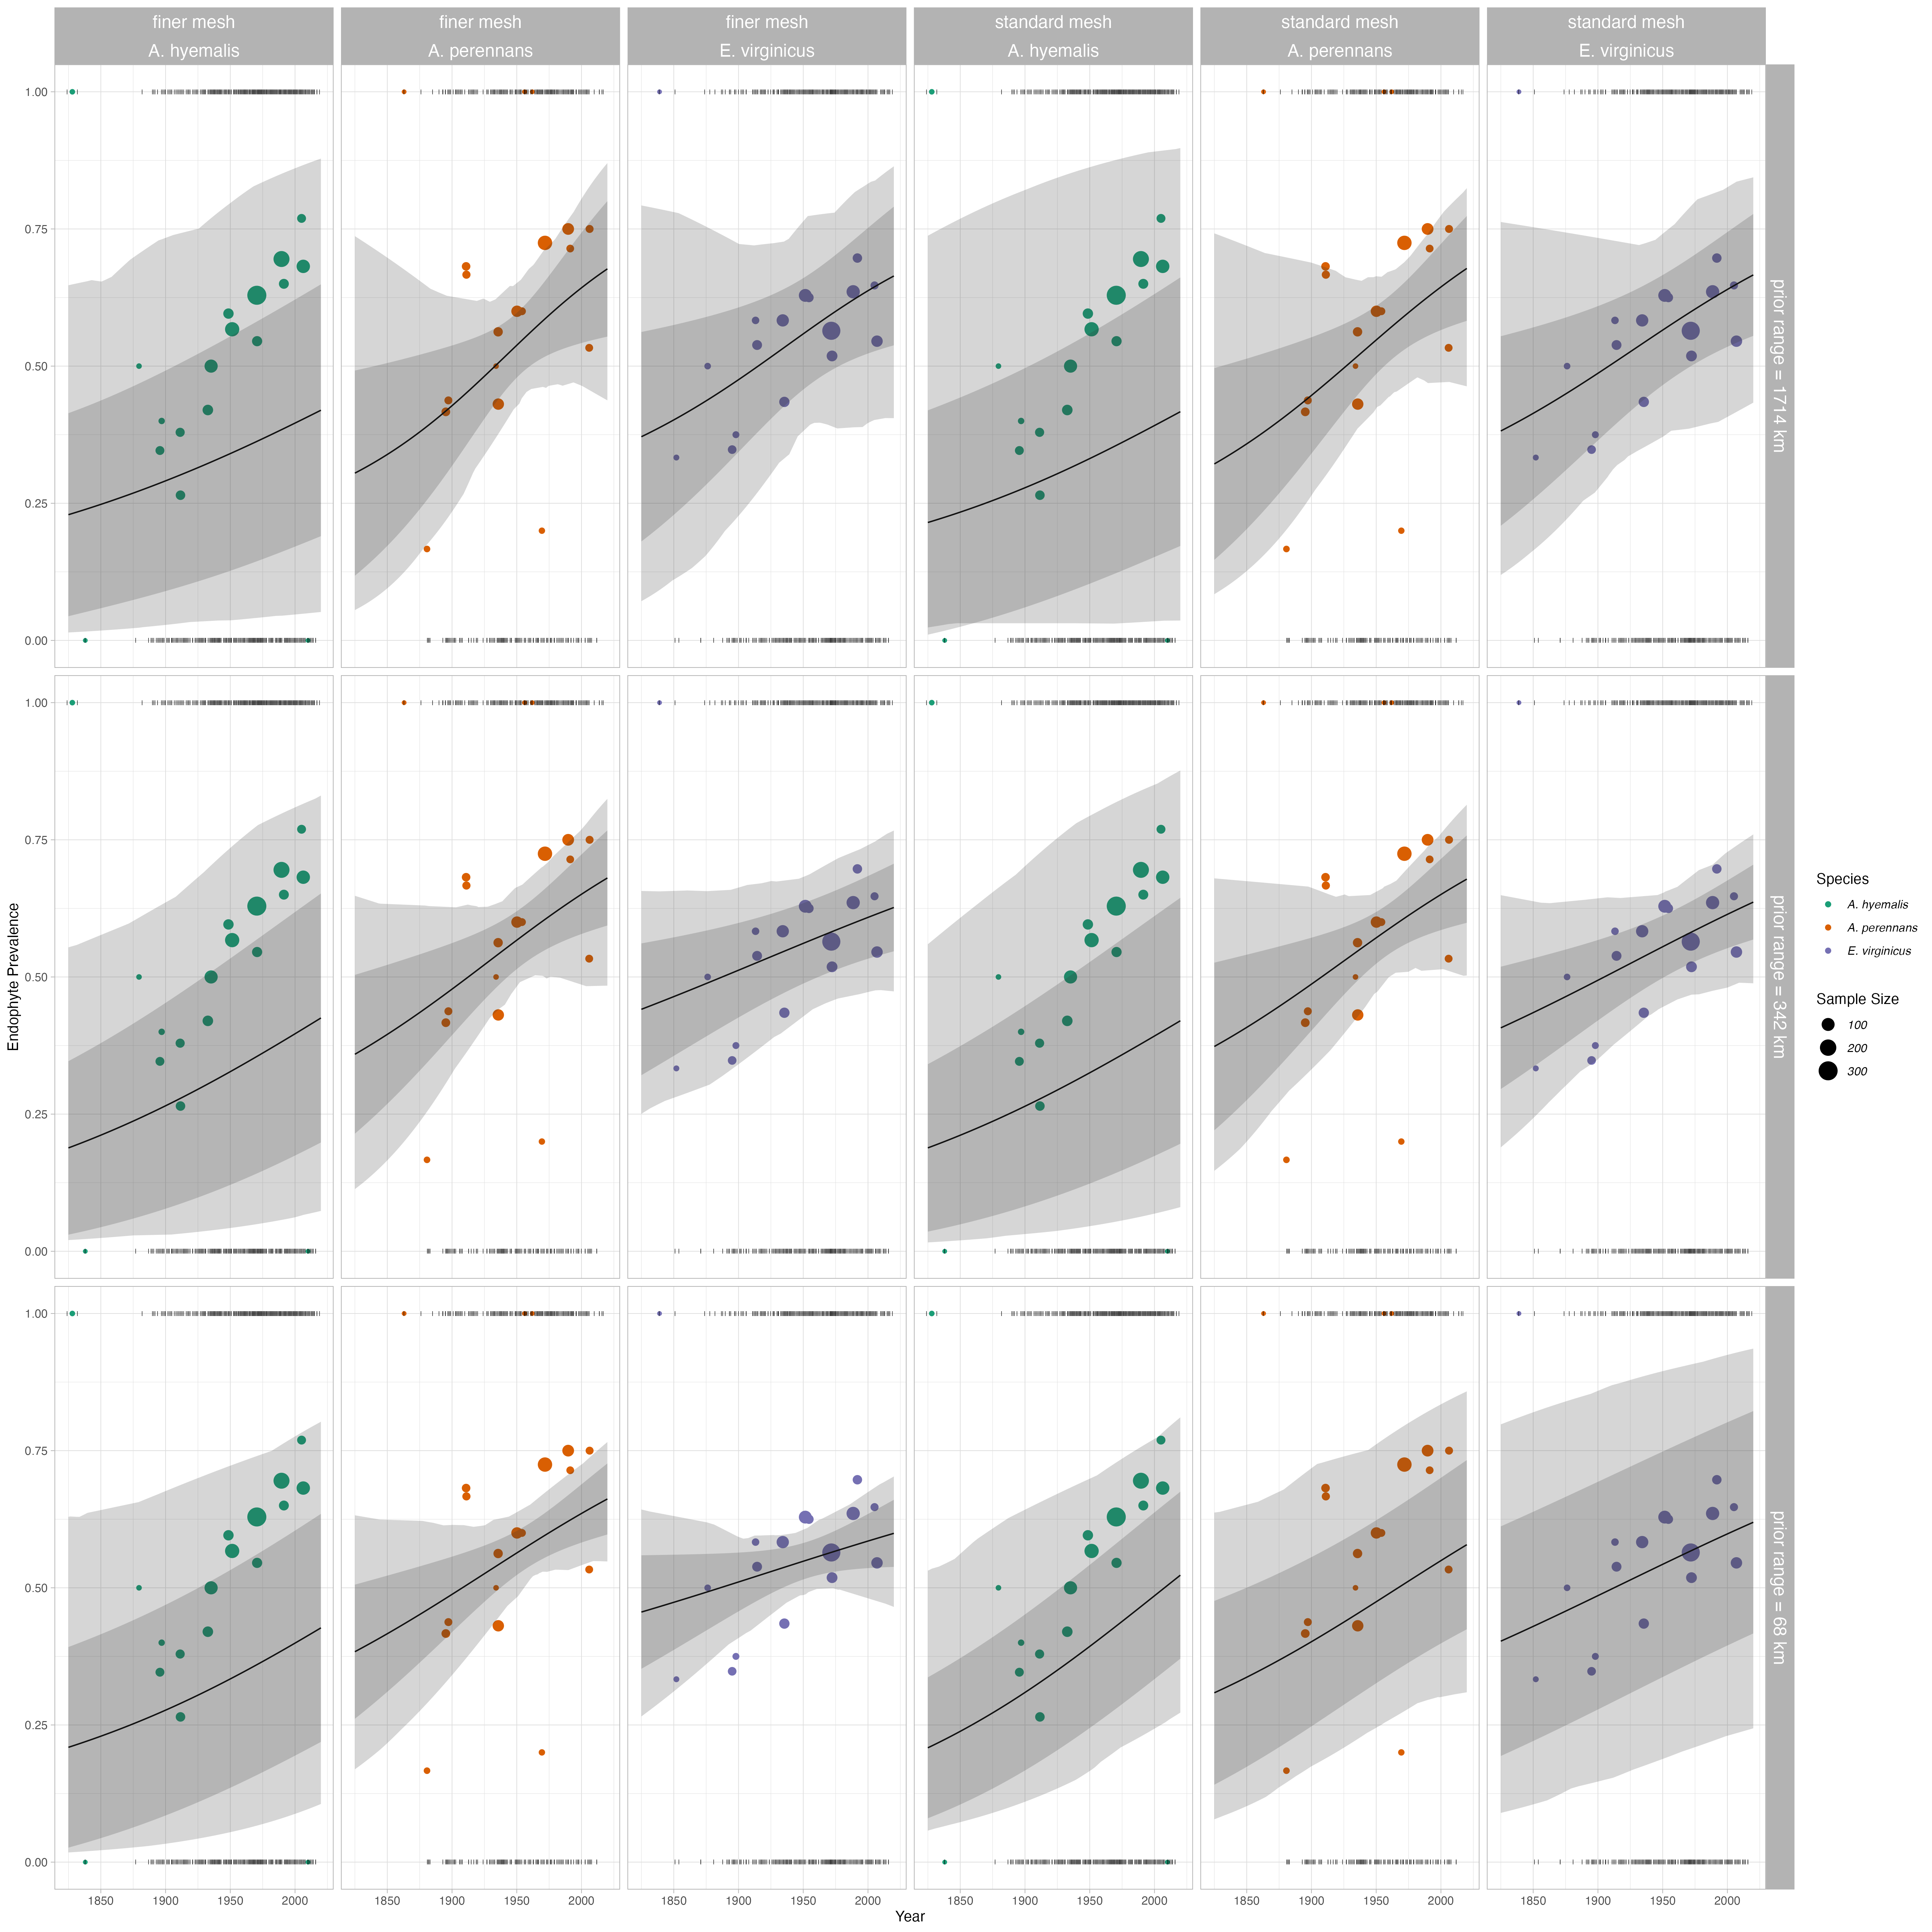
\includegraphics[width = \linewidth]{../Plots/prior_comparison_year_plot.png}
	\caption[Overall trend in endophyte prevalence evaluated for models with different range priors on spatially structured random effects, and for two different meshes]{\textbf{Overall trend in endophyte prevalence evaluated for models with different range priors on spatially structured random effects, and for two different meshes.} Note that these plots, as compared to Fig. 2 in main text, show mean trends and do not incorporate prediction uncertainty associated with collector and scorer random effects.}
	\label{fig:prior_year_plot}
\end{figure}

For spatially-varying temporal trends, we found that models with different priors predicted consistent spatial patterns in temporal trends, although the range of this prediction varied depending on the prior and mesh (Fig. \ref{fig:standard_comparison_svc_plot} - \ref{fig:finer_comparison_svc_plot}). One noteworthy result of this analysis is that combinations of prior choice and mesh can introduce instability in model fitting. This is evident in \ref{fig:standard_comparison_svc_plot} panel B and \ref{fig:finer_comparison_svc_plot} panel B, where the prior range is smaller than the minimum vertex length of the mesh.
Model fitting takes an extended time period and the model struggles to identify variation across space. Results with a set of prior ranges (Fig. \ref{fig:standard_comparison_svc_plot} -  A and C; Fig. \ref{fig:finer_comparison_svc_plot} - A and C) result in models that estimate trends across space of the same direction and order of magnitude, although the ``smoothness" of these predictions vary.

\begin{figure}[H]
	\centering
	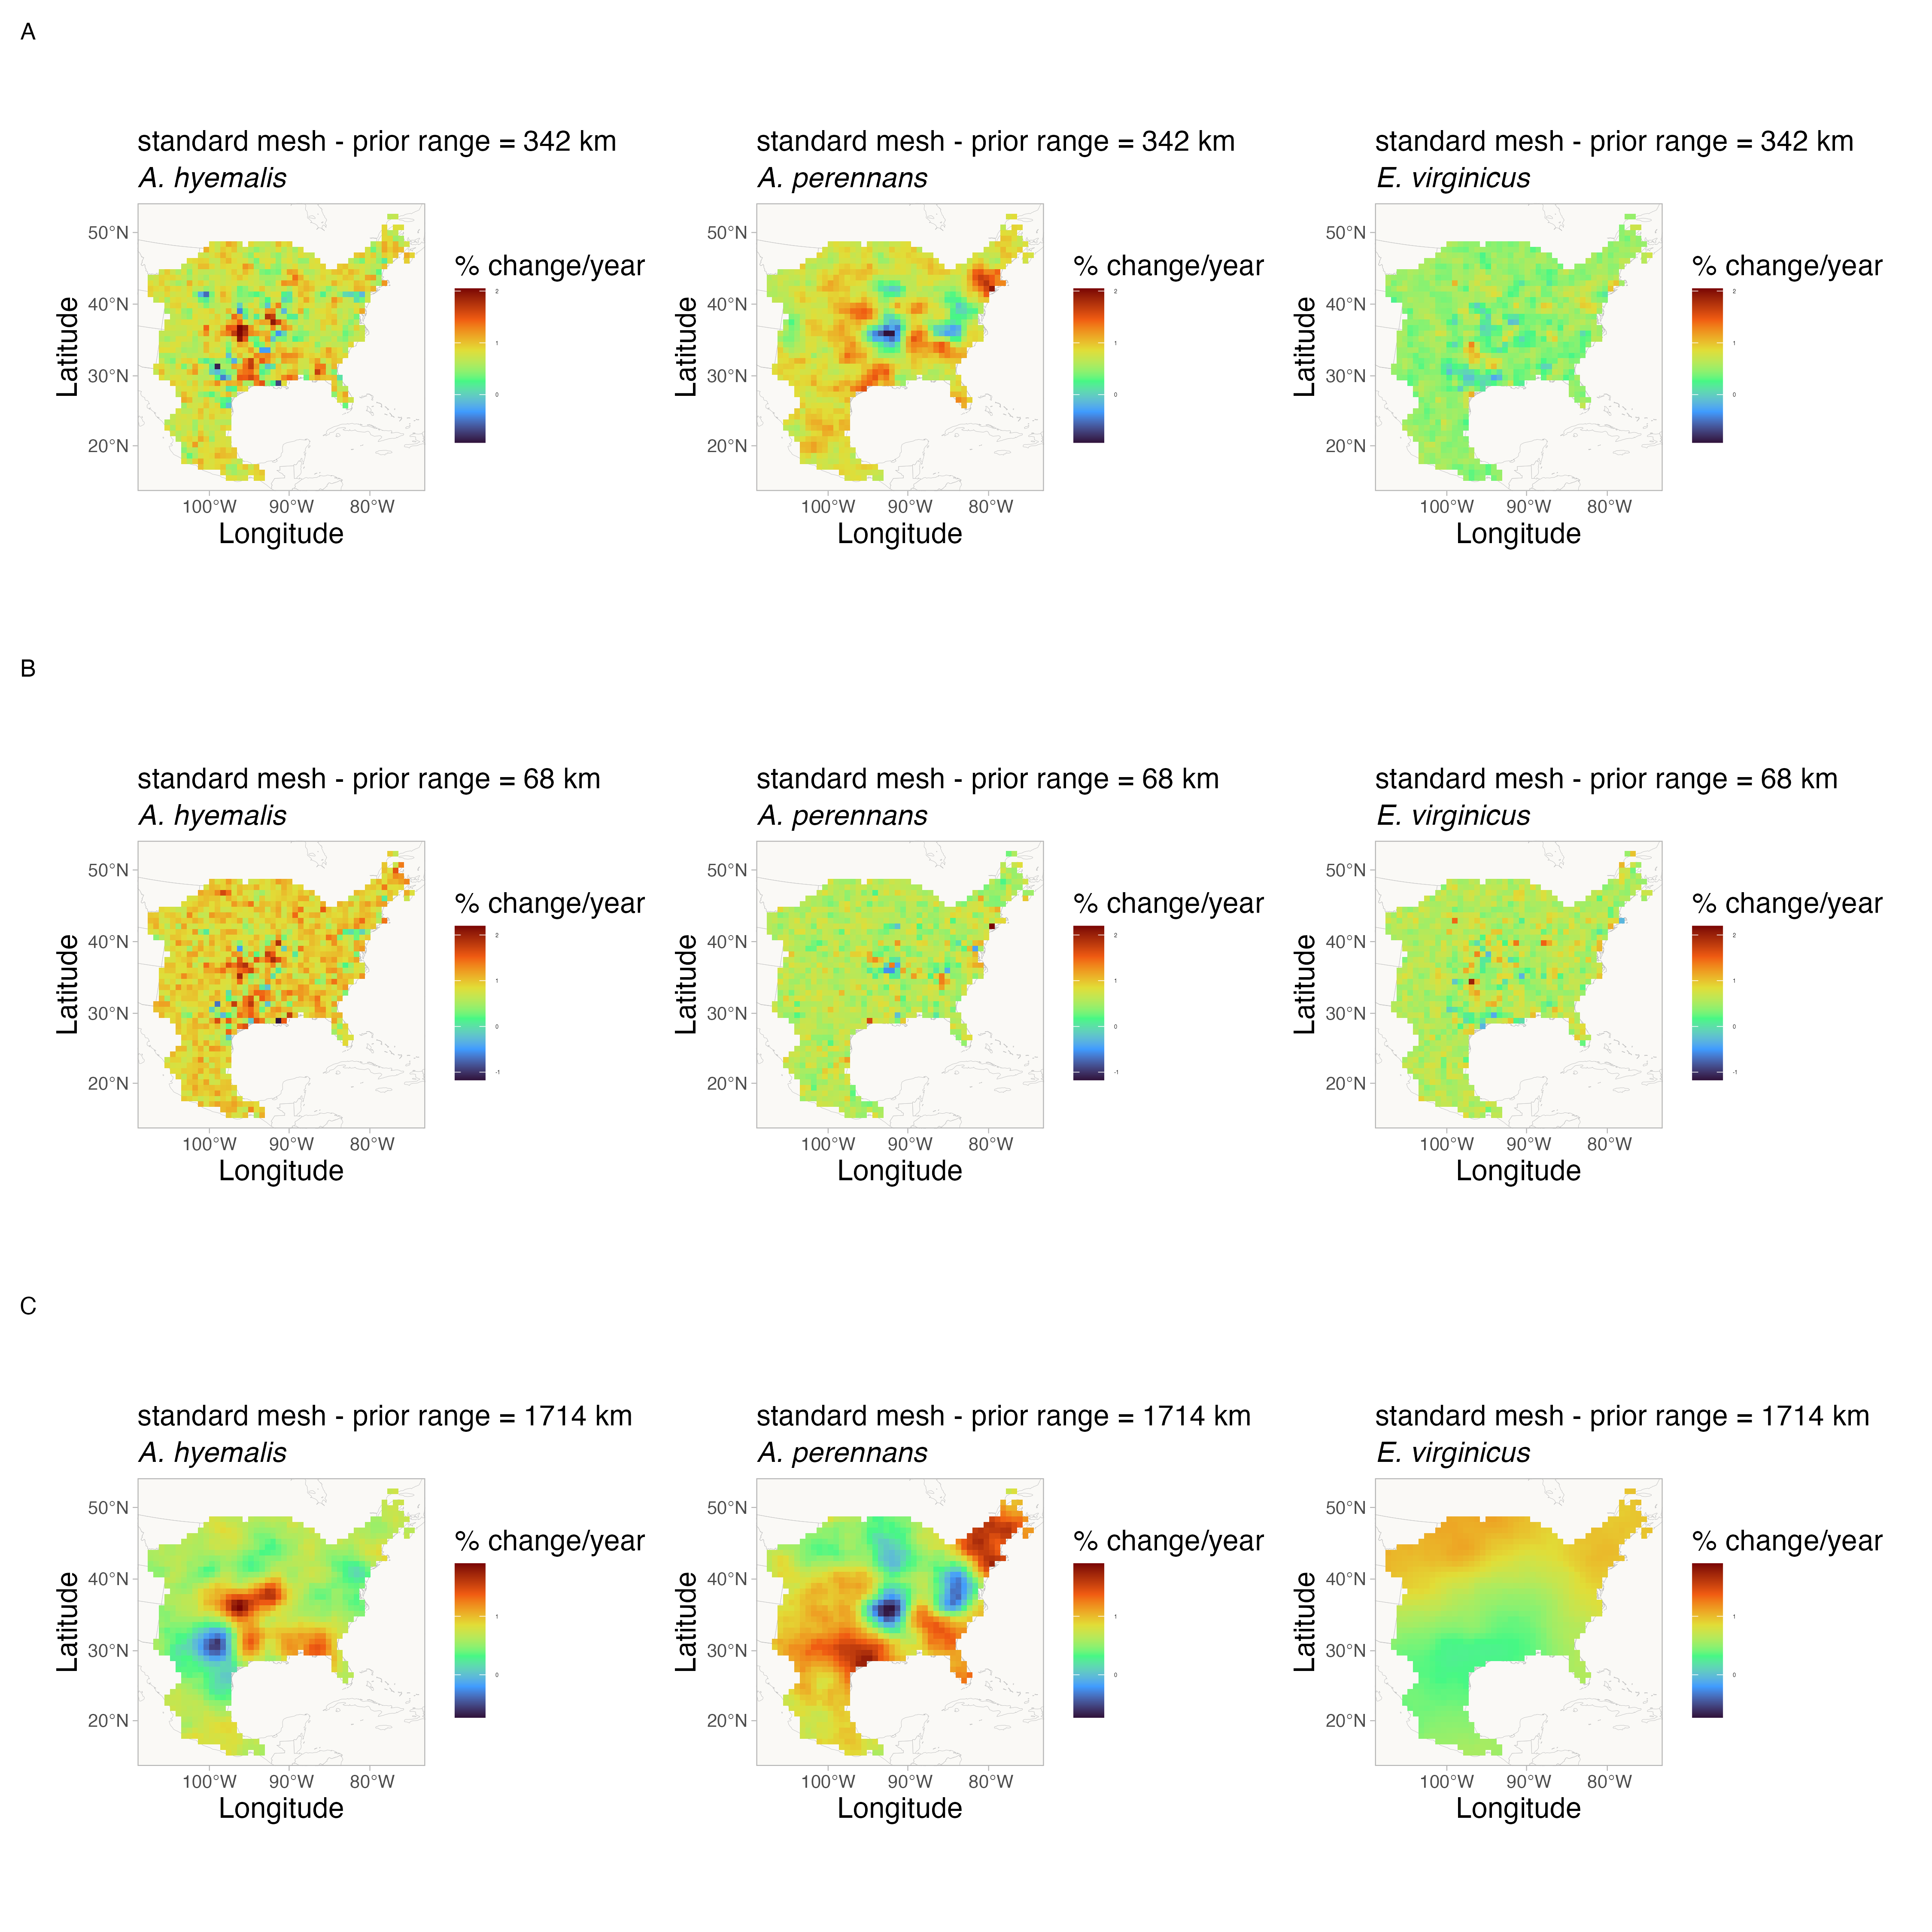
\includegraphics[width = .8\linewidth]{../Plots/standard_mesh_comparison_svc_plot.png}
	\caption[Spatially-varying trends in endophyte prevalence evaluated for models with different range priors on spatially structured random effects, and for the "standard" mesh]{\textbf{Spatially-varying trends in endophyte prevalence evaluated for models with different range priors on spatially structured random effects, and for the "standard" mesh.} Shading indicates the magnitude and direction of predicted trends for each of three host species for each of three prior ranges (rows A-C). Note that each plot has an individual scale bars.}
	\label{fig:standard_comparison_svc_plot}
\end{figure}


\begin{figure}[H]
	\centering
	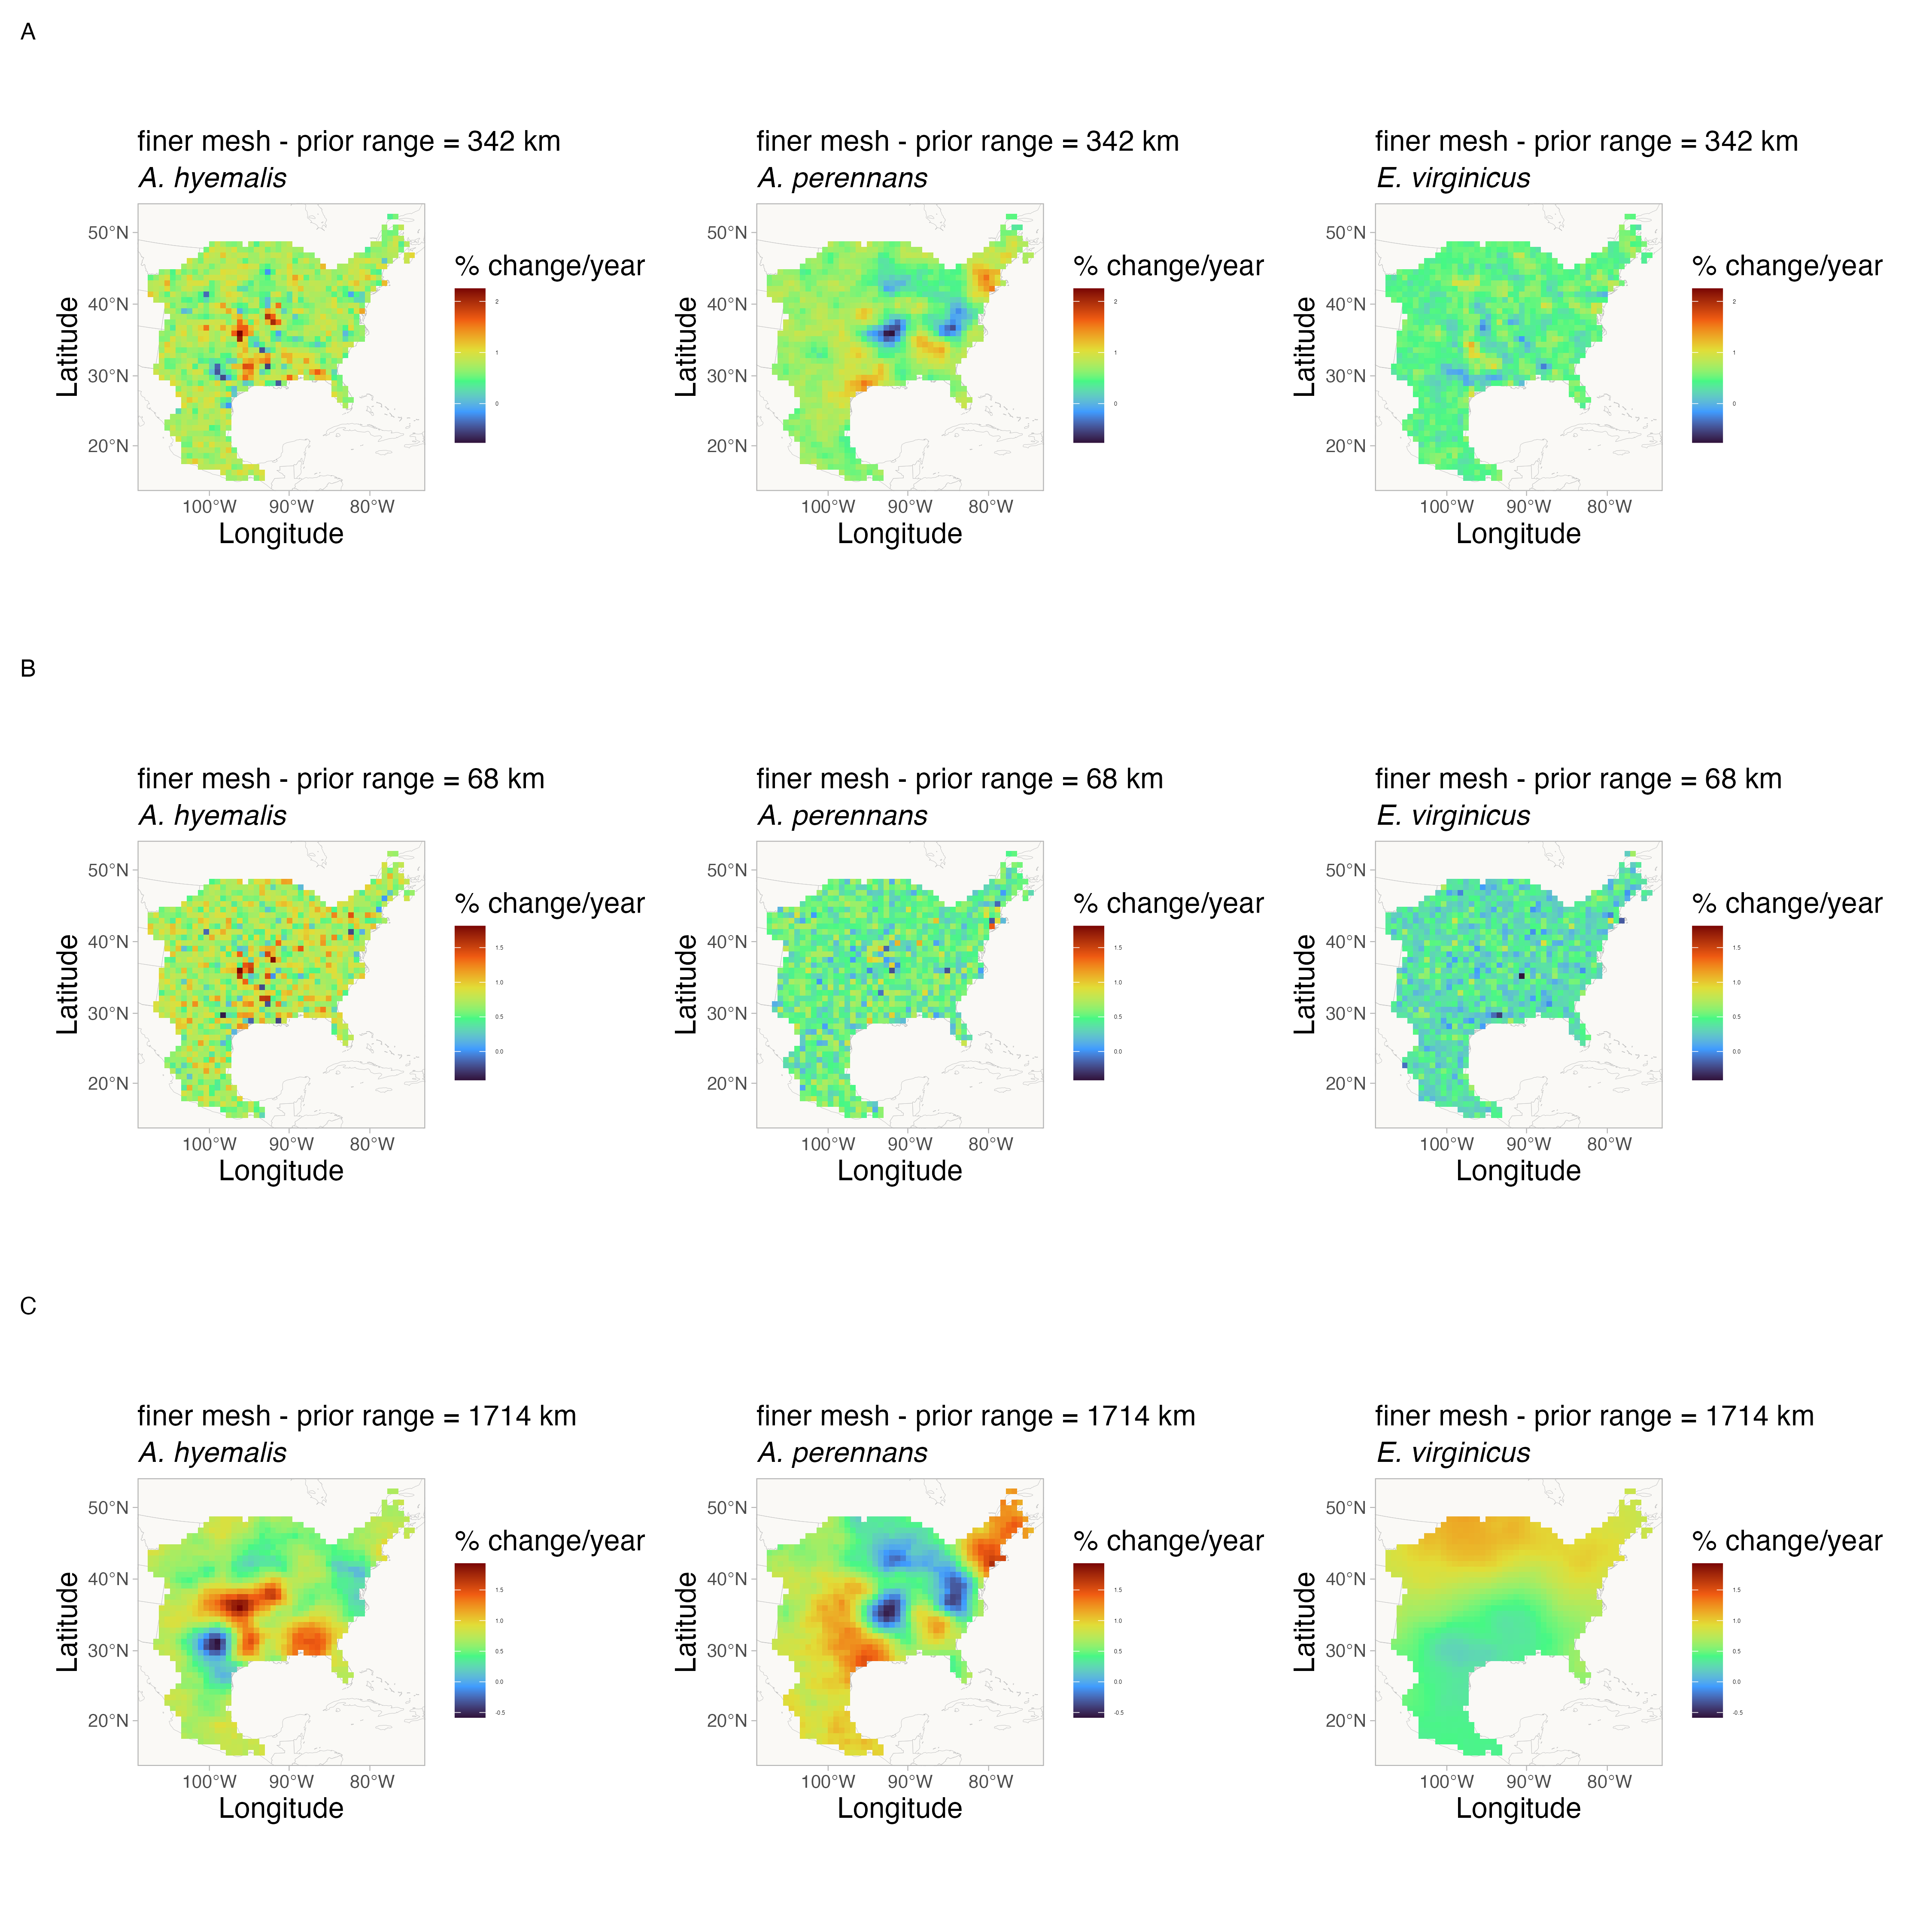
\includegraphics[width = .8\linewidth]{../Plots/finer_mesh_comparison_svc_plot.png}
	\caption[Spatially-varying trends in endophyte prevalence evaluated for models with different range priors on spatially structured random effects, and for the "finer" mesh]{\textbf{Spatially-varying trends in endophyte prevalence evaluated for models with different range priors on spatially structured random effects, and for the "finer" mesh.} Shading indicates the magnitude and direction of predicted trends for each of three host species for each of three prior ranges (rows A-C). Note that each plot has an individual scale bars.}
	\label{fig:finer_comparison_svc_plot}
\end{figure}


	% In most cases, authors should typeset supplementary material in a separate,
	% author-supplied PDF. For author-supplied PDFs, please consult the
	% AmNat_supp_template.tex document, available from
	% https://www.journals.uchicago.edu/journals/an/instruct 
	%
	% By contrast, the Appendix instructions below apply to cases in which
	% a brief appendix is to appear in print after the main body of the article.
	% That notably includes descriptions of methods, tables defining parameters,
	% and other material necessary for reproducing the MS's results.
	%
	% Please reset counters for the appendix (thus normally figure A1, 
	% figure A2, table A1, etc.).
	%
	% Most AmNat articles have no more than one print appendix. If your article
	% has more than one, counters for each appendix should match the letter of
	% that appendix. For example, tables in Appendix B should be numbered table B1, % table C2, etc. This applies to tables, equations, and figures.
	%
	% It's better not to use the \appendix command, because we have some
	% formatting peculiarities that \appendix conflicts with.
	
	%%%%%%%%%%%%%%%%%%%%%
	% Bibliography
	%%%%%%%%%%%%%%%%%%%%%
	% You can either type your references following the examples below, or
	% compile your BiBTeX database and paste the contents of your .bbl file
	% here. The amnatnat.bst style file should work for this---but please
	% let us know if you run into any hitches with it!
	%
	% If you upload a .bib file with your submission, please upload the .bbl
	% file as well; this will be required for typesetting.
	%
	% The list below includes sample journal articles, book chapters, and
	% Dryad references.
	\newpage{}
\bibliographystyle{plainnat}
\bibliography{endo_herbarium}
	
	\newpage{}
	

	
\end{document}

